\documentclass[12pt,a4paper]{article}
\usepackage[T1]{fontenc}
\usepackage{lmodern}
\usepackage[margin=2.45cm]{geometry}
\usepackage{amsmath,amssymb,bm,booktabs,graphicx,placeins,microtype,float}
\usepackage{listings,setspace,caption}
\setstretch{1.09}
\captionsetup{font=small,labelfont=bf,skip=9pt,width=.94\linewidth}
\captionsetup[table]{position=top}
\lstset{language=Python,basicstyle=\small\ttfamily,breaklines=true,columns=fullflexible,frame=single}
\usepackage[hidelinks]{hyperref}
\graphicspath{{figures/}}
\setlength{\parindent}{0pt}
\setlength{\parskip}{.62em plus .12em minus .08em}
\setlength{\textfloatsep}{20pt plus 3pt minus 3pt}
\setlength{\intextsep}{16pt plus 3pt minus 3pt}
\setlength{\floatsep}{17pt plus 3pt minus 3pt}
\makeatletter
\setlength{\@fptop}{16pt}
\setlength{\@fpsep}{23pt plus 5pt}
\setlength{\@fpbot}{0pt plus 1fil}
\makeatother
\renewcommand{\arraystretch}{1.20}
\raggedbottom
\emergencystretch=1em
\title{Cartesian End-Effector Control and Randomized Block Stacking\\with a Franka Emika Panda in MuJoCo}
\author{Hamza Demir\\\small Supervisor: Jos\'e Luis Holgado Alvarez}
\date{18 November 2026}
\begin{document}
\maketitle
\begin{abstract}
This report evaluates torque-level Cartesian control of a seven-joint Franka Emika Panda in MuJoCo. A finite-difference check of the geometric Jacobian yielded a maximum error of $2.774\times10^{-7}$, and damped least-squares inverse kinematics converged for all five reachable test poses. Across 15 tracking trials, mean position RMSE ranged from 4.86 to 9.87 mm across three path families. Step, speed, and load tests revealed distinct limits: tracking exceeded the 50 mm peak-error threshold on the figure-eight at four times nominal speed, and a constant downward force equivalent to a 1 kg load produced a 50.74 mm residual error. The scripted manipulator completed both requested towers in all ten randomized five-block episodes within a 120 s horizon. Mean episode placement error was $14.87\pm0.70$ mm, with larger offsets on higher levels. The experiments use a simulated robot and exact block positions from the simulator.
\end{abstract}
\clearpage
\setcounter{tocdepth}{2}
\begingroup
\singlespacing
\setlength{\parskip}{0pt}
\tableofcontents
\endgroup

\clearpage
\section{Introduction}
Cartesian control expresses manipulation goals in terms of hand position and orientation. The Panda's seven arm joints leave one redundant degree of freedom for a full six-dimensional pose task. This work uses that redundancy to bias the arm toward a preferred posture while tracking workspace references. The controller follows the Jacobian-transpose wrench mapping associated with operational-space control~\cite{khatib1987}. The evaluation moves from numerical kinematics to repeated free-space tracking, dynamic limits, and randomized contact manipulation.

\subsection{Objectives and evaluation design}
The evaluation follows four stages. Numerical checks first establish that the differential kinematics and pose solver are internally consistent. Free-space experiments then measure how accurately a torque-controlled arm follows Cartesian references. Separate step, timing and force tests vary one class of input at a time to expose performance limits. Finally, grasping and stacking exercise the same control architecture with contact, gripper commands and randomized tasks.

The measurements have different experimental units. IK convergence is counted per target pose. Tracking and dynamic statistics summarize independent seeded trials, with one peak or RMSE computed per trial before aggregation. Stacking success is counted per episode, whereas placement errors may also be grouped by individual block or tower level. Reporting these counts alongside each result keeps repeated physics samples from being interpreted as independent trials.

\section{Robot and Simulation Model}
The MuJoCo scene contains a Panda arm, a parallel-jaw gripper, a table, and five free 40 mm cubes. The arm and gripper use the Franka Emika Panda MJCF description and meshes from MuJoCo Menagerie~\cite{menageriePanda}. The current model has 19 bodies, 14 joints, 44 generalized positions, 39 generalized velocities, and eight actuators. The seven arm actuators are torque-commanded during the experiments, and the fingers share a gripper actuator. The simulation advances in 2 ms steps and the tracking and controller-limit tests update the command every 10 ms. MuJoCo provides dynamics, collision handling and contact simulation~\cite{todorov2012}.
The free blocks each contribute seven generalized position coordinates (translation and a unit quaternion) and six velocity coordinates. This accounts for the difference between the position and velocity dimensions. The fingers contribute two joints but share one control input. The model uses RK4 integration and downward gravity of $9.81\,\mathrm{m/s^2}$. Cartesian references and measurements use world axes, including the angular component of the geometric Jacobian.

The scene also includes a floor, fixed front camera and visual target marker. The marker serves the original Cartesian interface. The ordered tower task uses two separately defined world-coordinate targets. The environment resolves the hand body by name and reads the position and velocity addresses of the arm joints from the loaded model. These address lists keep free joints and finger joints out of the arm Jacobian and the torque command. The logged experiments use Python 3.11, MuJoCo 3.9.0 and NumPy, with Gymnasium providing the environment interface.

\subsection{Arm joint limits}
\begin{table}[!htbp]
\centering
\caption{Panda arm joint limits read from the loaded MuJoCo model.}
\begin{tabular}{lrr}
\toprule
Joint & Lower limit (rad) & Upper limit (rad)\\
\midrule
joint1 & -2.9 & 2.9\\
joint2 & -1.8 & 1.8\\
joint3 & -2.9 & 2.9\\
joint4 & -3.1 & -0.07\\
joint5 & -2.9 & 2.9\\
joint6 & -0.018 & 3.8\\
joint7 & -2.9 & 2.9\\
\bottomrule
\end{tabular}
\end{table}

The reset configuration was changed from the invalid all-zero posture to
\begin{equation}
\bm q_{\mathrm{home}}=[0,0,0,-1.57079,0,1.57079,-0.7853]^T,
\end{equation}
which lies inside the arm joint limits.



\subsection{Gymnasium Cartesian pose interface}
The original Cartesian command path is available through the environment's \texttt{pose} mode. Its action is
\[
\bm a=[x_d,y_d,z_d,q_w,q_x,q_y,q_z]^T,
\]
with a world-frame target position and a scalar-first quaternion. The environment rescales the quaternion by its norm with a small numerical floor, converts it to a rotation matrix, solves full-pose IK and writes seven joint position targets. The step advances MuJoCo once and returns the IK convergence flag, iteration count and final IK errors in the information dictionary.

The observation has 30 values: seven arm positions, seven arm velocities, hand position and quaternion, first-cube position, visual target position and the displacement from hand to first cube. This observation supports the original single-cube interface. The five-block stack reads all five cube positions through explicit environment accessors. The trajectory and manipulation experiments advance the simulator through the torque-control method described below.

\clearpage
\section{Kinematics and Validation}
\subsection{Forward kinematics}
For arm coordinates $\bm q\in\mathbb{R}^7$, the end-effector pose is represented by
\begin{equation}
{}^{0}\!T_E(\bm q)=
\begin{bmatrix}
{}^{0}\!R_E(\bm q) & {}^{0}\!\bm p_E(\bm q)\\
\bm 0^T & 1
\end{bmatrix}.
\end{equation}

The environment evaluates both position and orientation at the hand body. When a candidate joint vector is supplied, the current MuJoCo state is saved, the candidate configuration is evaluated with \texttt{mj\_forward}, and the original state is restored. This makes the function suitable for target generation and IK validation without corrupting the active simulation state.



\subsection{End-effector Jacobian}
The geometric Jacobian maps joint velocity to spatial twist:
\begin{equation}
\begin{bmatrix}\bm v_E\\\bm\omega_E\end{bmatrix}
=J(\bm q)\dot{\bm q},
\qquad
J=\begin{bmatrix}J_v\\J_\omega\end{bmatrix}\in\mathbb{R}^{6\times7}.
\end{equation}

The implementation uses MuJoCo's body Jacobian and extracts the seven arm degrees of freedom. Both translational and rotational blocks are retained. Numerical validation perturbs each joint by $\epsilon=10^{-6}\,\mathrm{rad}$ and compares the analytical columns against finite differences of position and orientation at the home posture.

\begin{table}[!htbp]
\centering
\caption{Finite-difference Jacobian validation.}
\begin{tabular}{lr}
\toprule
Metric & Maximum absolute error\\
\midrule
Translational block & $2.774\times10^{-7}$\\
Rotational block & $3.967\times10^{-10}$\\
Complete $6\times7$ Jacobian & $2.774\times10^{-7}$\\
\bottomrule
\end{tabular}
\end{table}



\subsection{Inverse kinematics}

For desired pose $(\bm p_d,R_d)$ and current pose $(\bm p,R)$, the position error is
\begin{equation}
\bm e_p=\bm p_d-\bm p.
\end{equation}



Let $Q=R^TR_d$. The controller and IK solver use the world-frame orientation error $\bm e_R=\tfrac12 R\,(Q-Q^T)^\vee$, where $\vee$ extracts the vector from a skew-symmetric matrix. The complete task error is
\begin{equation}
\bm e=\begin{bmatrix}\bm e_p^T & \bm e_R^T\end{bmatrix}^T\in\mathbb{R}^6.
\end{equation}


The inverse-kinematics solver uses a damped least-squares inverse~\cite{wampler1986} to limit the gain near kinematic singularities. For Jacobian $J$ and damping $\lambda$, the inverse is
\begin{equation}
J^{\#}=J^T\left(JJ^T+\lambda^2I\right)^{-1},
\end{equation}
\begin{equation}
\Delta\bm q=J^{\#}\bm e+k_N\left(I-J^{\#}J\right)(\bm q_{\mathrm{pref}}-\bm q).
\end{equation}

The update norm is limited, a step size is applied, and the resulting joint vector is clipped to the model limits after every iteration. The validation settings were: maximum 1000 iterations, damping 0.03, step size 0.7, maximum update norm 0.20 rad, position tolerance $10^{-4}\,\mathrm{m}$, orientation tolerance $10^{-3}\,\mathrm{rad}$, and null-space gain 0.02.

\subsection{Five-pose numerical validation}
Five reachable poses were produced using seed 7, with uniform perturbations of up to 0.35 rad per home joint and clipping to the model limits. Each pose was solved from the same home configuration.

\begin{table}[!htbp]
\centering
\caption{Full-pose inverse-kinematics validation results.}
\scriptsize
\begin{tabular}{ccccccc}
\toprule
Test & Conv. & Iter. & Initial pos. (m) & Initial ori. (rad) & Final pos. (m) & Final ori. (rad)\\
\midrule
1 & yes & 11 & $2.779\times10^{-1}$ & $7.077\times10^{-1}$ & $4.317\times10^{-5}$ & $8.346\times10^{-5}$\\
2 & yes & 9  & $2.097\times10^{-1}$ & $5.962\times10^{-1}$ & $5.189\times10^{-5}$ & $1.437\times10^{-4}$\\
3 & yes & 10 & $2.339\times10^{-1}$ & $7.446\times10^{-1}$ & $4.239\times10^{-5}$ & $1.116\times10^{-4}$\\
4 & yes & 11 & $3.505\times10^{-1}$ & $9.488\times10^{-1}$ & $5.896\times10^{-5}$ & $1.838\times10^{-4}$\\
5 & yes & 9  & $9.862\times10^{-2}$ & $5.285\times10^{-1}$ & $3.753\times10^{-5}$ & $1.767\times10^{-4}$\\
\bottomrule
\end{tabular}
\end{table}

All five solutions respected the joint limits and converged in 9--11 iterations. Mean final position and orientation errors were $4.679\times10^{-5}$ m and $1.399\times10^{-4}$ rad. The corresponding maxima were $5.896\times10^{-5}$ m and $1.838\times10^{-4}$ rad. Convergence is checked using the geodesic rotation angle
\[
\theta=\cos^{-1}\!\left(\operatorname{clip}\left(\tfrac{\operatorname{tr}(R^TR_d)-1}{2},-1,1\right)\right).
\]
The skew-based orientation vector drives the update, while the geodesic angle provides the rotational tolerance and the reported orientation error.

\subsection{Interpretation of the kinematic checks}
The finite-difference experiment checks the selected body, column indexing and coordinate convention of the implemented Jacobian at the home configuration. Because the position and rotation differences come from the same simulator model, this is a numerical consistency check of the implemented kinematics. The five IK targets are generated by forward kinematics, so their reachability is known by construction. This design exercises the solver with a common initial posture and different target displacements. Contact, unreachable targets and multiple IK branches lie outside this validation set.

Damping regularizes the inverse near small singular values. For singular value $\sigma_i$, the corresponding gain in $J^{\#}$ is $\sigma_i/(\sigma_i^2+\lambda^2)$. This bounds the inverse gain but also reduces correction along weakly controllable directions. The damped posture term can influence the primary task because $I-J^{\#}J$ is an approximate null-space projection. Per-iteration joint clipping enforces joint bounds but gives no guarantee that a clipped iterate will converge.

\section{Classical End-Effector Controller}
The manipulation experiments use torque-level six-dimensional task-space proportional--derivative control. The environment disables the seven arm position servos and writes direct arm torque to the corresponding entries of \texttt{qfrc\_applied}. The gripper keeps its original actuator command. For desired pose $(\bm p_d,R_d)$ and desired twist $(\bm v_d,\bm\omega_d)$, the task wrench is
\begin{equation}
\bm w =
\begin{bmatrix}
K_{p,p}(\bm p_d-\bm p)+K_{d,p}(\bm v_d-\bm v)\\
K_{p,R}\bm e_R+K_{d,R}(\bm\omega_d-\bm\omega)
\end{bmatrix}.
\end{equation}
The primary joint torque is $J^T\bm w$. A damped posture torque $N^T[K_{p,N}(\bm q_{\rm pref}-\bm q)-K_{d,N}\dot{\bm q}]$, where $N=I-J^{\#}J$, is added together with the arm entries of MuJoCo's bias forces, and the resulting commands are clipped to the declared limits $[87,87,87,87,12,12,12],\mathrm{N\,m}$.


The tracking and controller-limit experiments share a gain set. Stacking uses a second set. Both use damping $0.05$.

\begin{table}[!htbp]
\centering\small
\caption{Task-space PD gains used in the tracking and stacking experiments.}
\begin{tabular}{lcc}
\toprule
Gain & Tracking and controller limits & Stacking\\
\midrule
Translation $K_{p,p}$ & $(150,150,185)$ & $(180,180,220)$\\
Translation $K_{d,p}$ & $(30,30,34)$ & $(28,28,34)$\\
Rotation $K_{p,R}$ & $(30,30,25)$ & $(45,45,35)$\\
Rotation $K_{d,R}$ & $(10,10,9)$ & $(8,8,7)$\\
Posture $(K_{p,N},K_{d,N})$ & $(5,2)$ & $(18,5)$\\
\bottomrule
\end{tabular}
\end{table}

\subsection{Control cycle and measured signals}
At each control update, the implementation reads the hand pose, joint positions and velocities. The geometric Jacobian maps arm joint velocity to hand twist. The Cartesian PD law combines pose error with the difference between commanded and measured twist, then maps the resulting wrench to arm torque. The controller adds the preferred-posture and bias terms before clipping each actuator command. During tracking and the dynamic studies, the command is held over five physics substeps. A sample is marked saturated if any raw joint torque exceeds its configured limit.

The wrench mapping uses $J^T$ directly. Its response therefore varies with robot configuration and effective inertia. The Cartesian stiffness sets the approximate tradeoff between tracking error and force demand. Damping shapes the transient response, while the bias term accounts for gravity and velocity-dependent forces represented in the simulator. The static-load experiment probes forces missing from that model.

\subsection{Free-space pose-reaching check}
The standalone torque-control check moves the hand from its home pose by $(0,0.12,0.04)$ m with constant desired orientation. The command uses a 4 s cubic move followed by a 1 s hold. The controller updates every 2 ms. In the 2,500 archived samples, the peak, RMS and final position errors were 12.91, 9.10 and 12.47 mm. Peak orientation error was $0.644^\circ$, and no sample triggered torque clipping. This single smooth move checks the torque interface before the repeated step and path experiments.

\begin{figure}[!htbp]
\centering
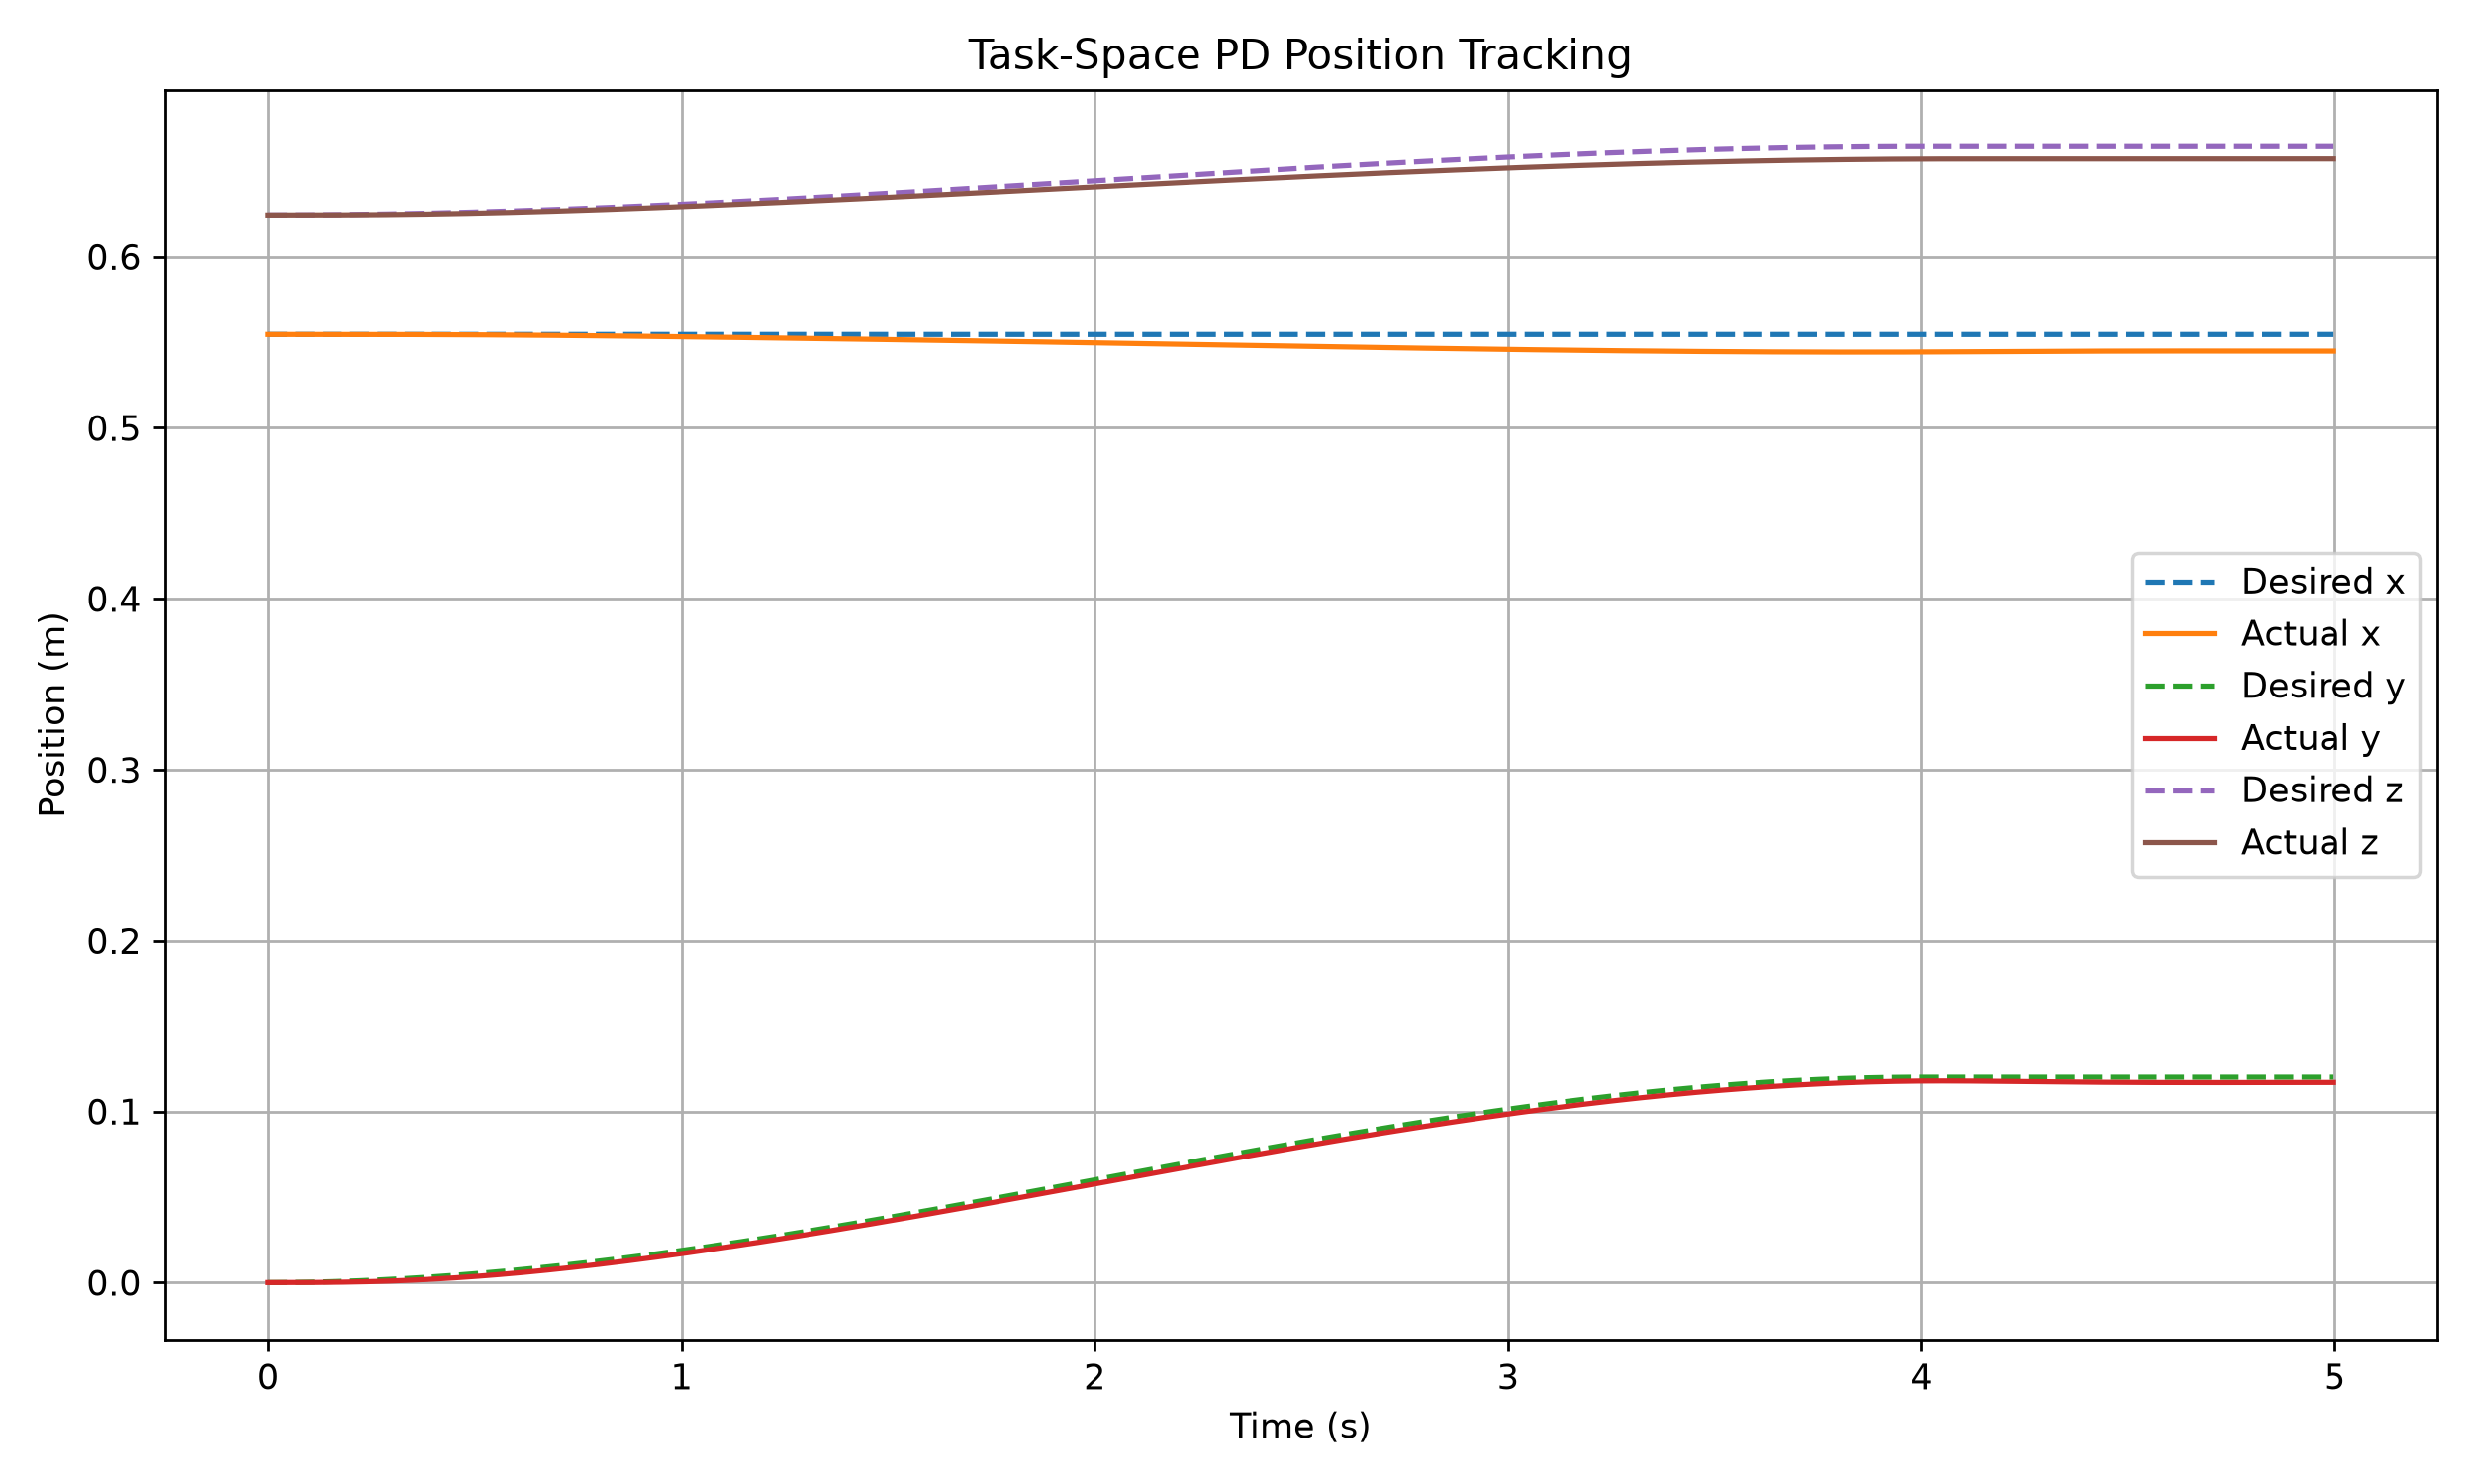
\includegraphics[width=.48\linewidth]{pose_reaching_position.png}
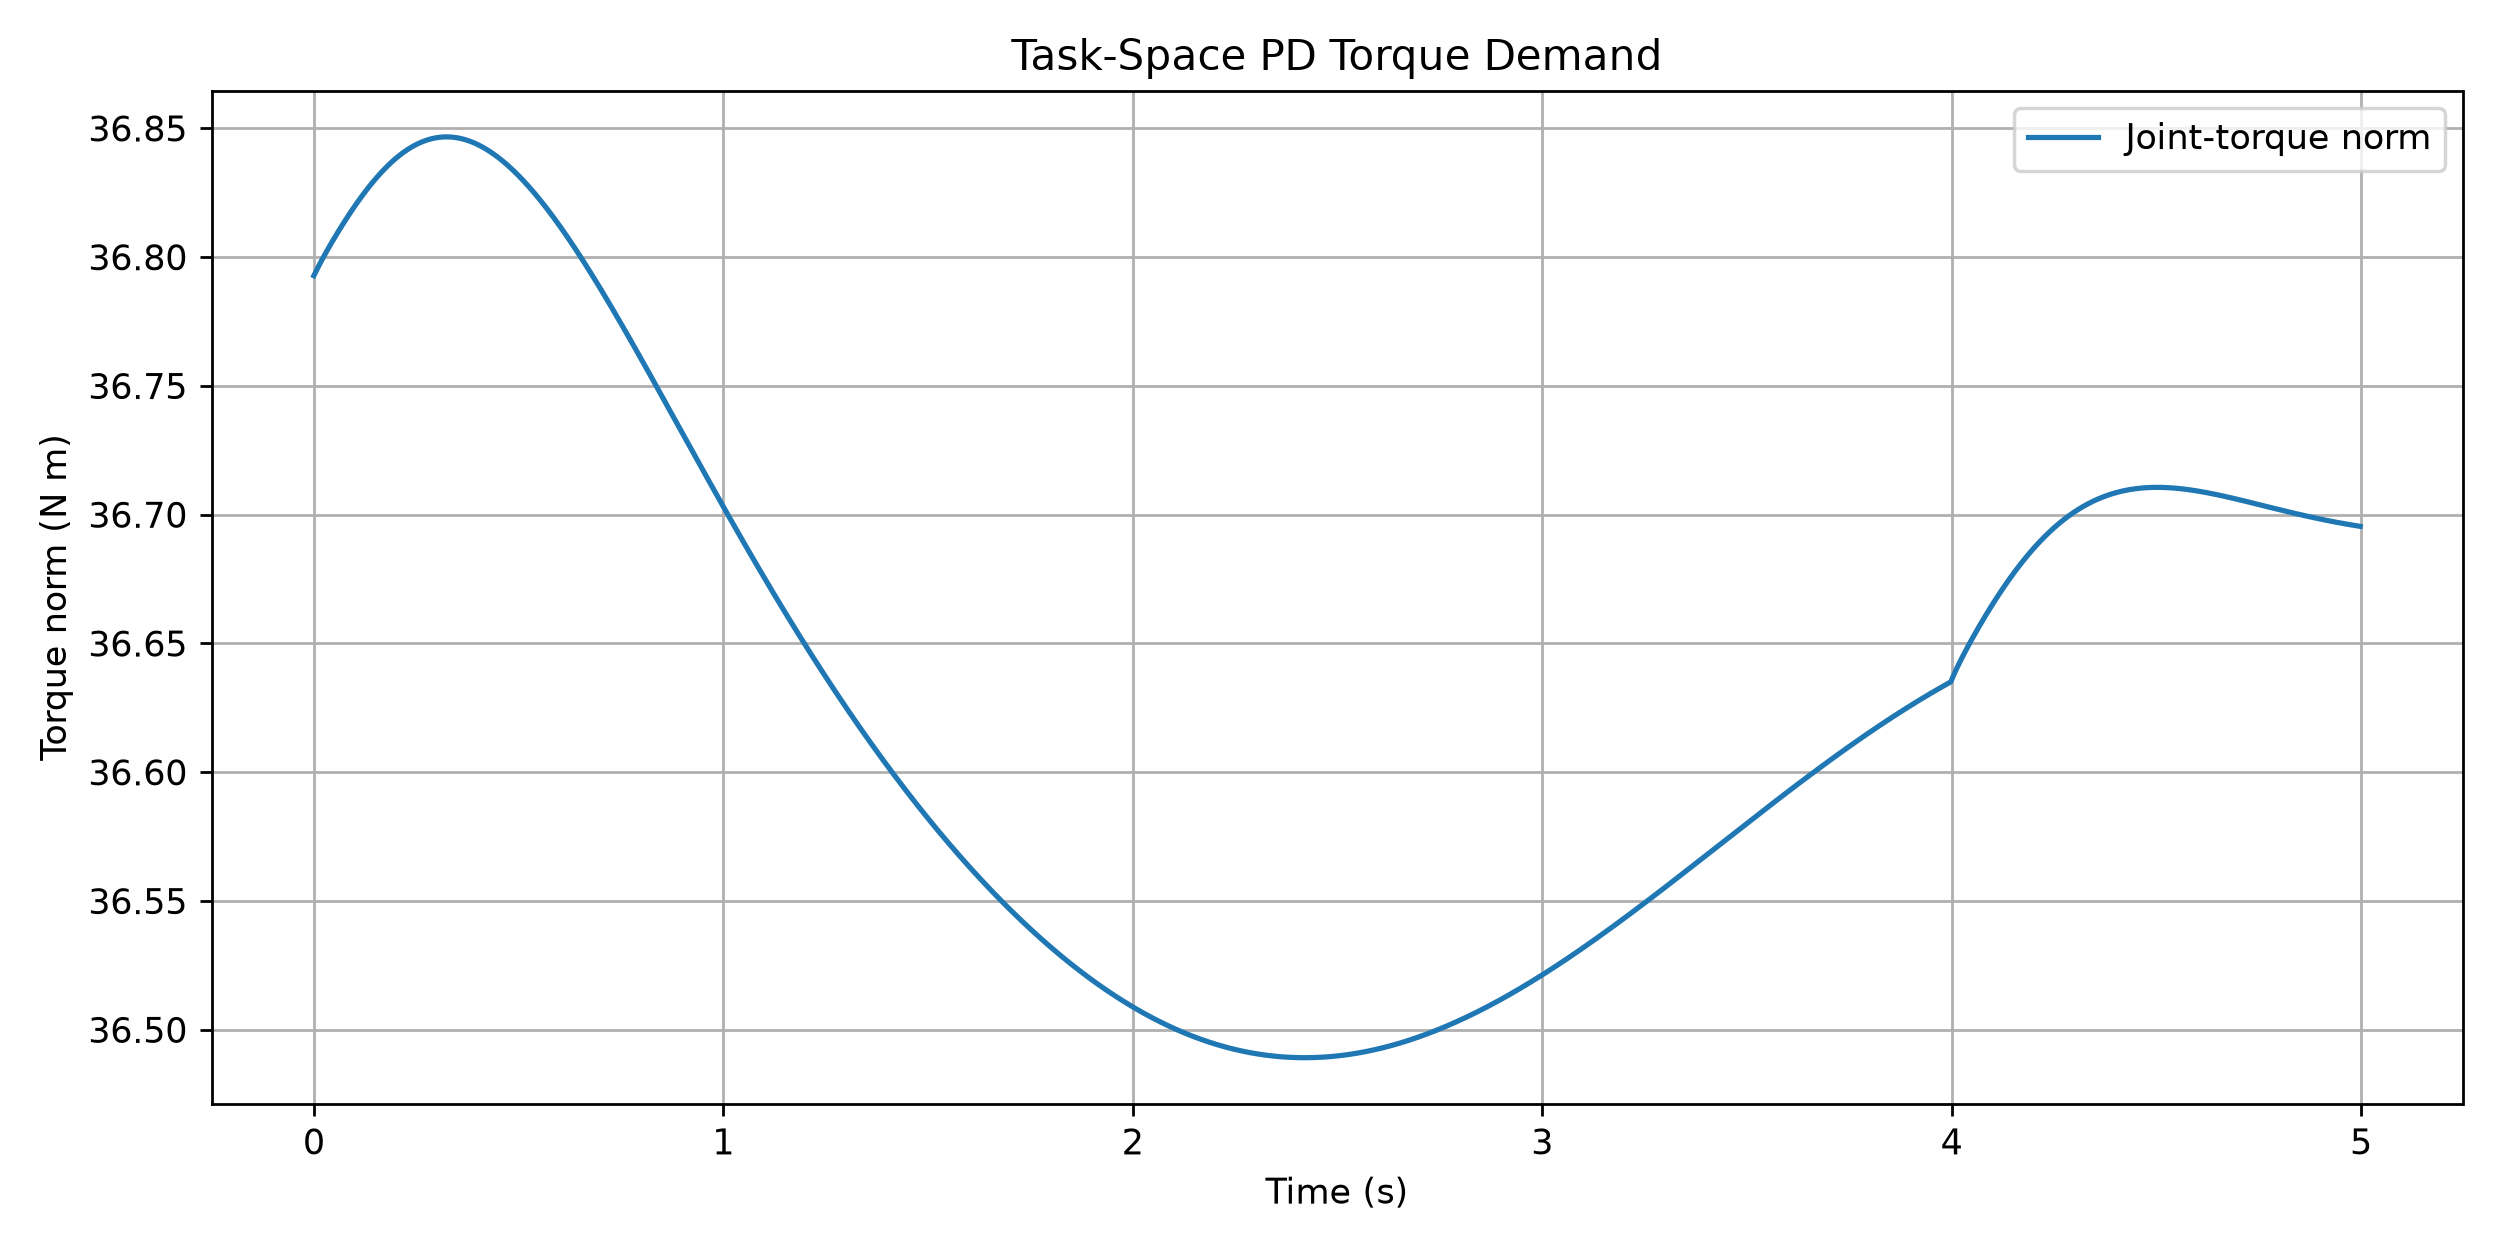
\includegraphics[width=.48\linewidth]{pose_reaching_torque.png}
\caption{Position tracking and commanded arm-torque norm in the standalone free-space check. The norm summarizes all seven commands. Clipping is evaluated per joint.}
\end{figure}

\subsection{Waypoint tracking during development}
The waypoint experiment uses four sampled Cartesian points and serves as a baseline before the repeated analytic-path study. Candidates are drawn uniformly from $[0.46,0.60]$ m in $x$, $[-0.16,0.16]$ m in $y$ and $[0.66,0.74]$ m in $z$. The first candidate must be within 100 mm of the starting hand, and successive points must be at least 100 mm apart. Full-pose IK screens each point at the fixed hand orientation. The simulator starts with a seeded perturbation of up to 0.06 rad per arm joint, clipped to the limits. Path logging starts after the hand remains within 5 mm and $2^\circ$ of the first point for the configured settling interval of 0.25 s. The script allows up to 15 s for this step. The first point is appended to close the loop, giving four segments and 16 s of commanded motion.

Each straight segment uses linear segments with parabolic blends~\cite{siciliano2009}. Let $T$ be segment duration, $t_b$ the blend duration and $a=1/[t_b(T-t_b)]$. The normalized displacement is
\[
s(t)=
\begin{cases}
at^2/2 & 0\le t<t_b,\\
at_b(t-t_b/2) & t_b\le t\le T-t_b,\\
1-a(T-t)^2/2 & T-t_b<t\le T.
\end{cases}
\]
The hand reference follows $\bm p(t)=\bm p_0+s(t)(\bm p_1-\bm p_0)$. Differentiating yields the velocity and acceleration references. With the nominal 4 s segment and 1 s blends, velocity starts and ends at zero, while acceleration changes piecewise between positive, zero and negative values. The waypoint experiment therefore exercises stop-and-go motion at changes in direction, complementing the analytic paths, which follow a continuous phase.

The archived run reported in the earlier draft settled in approximately 1.50 s. The reported position errors were 9.92 mm peak, 4.97 mm mean, 5.23 mm RMS and 3.41 mm at the end of the path. Peak rotational error was $0.637^\circ$, and the draft reported no torque clipping. Those values describe one historical development run. In four current-code checks, seed 19 settled in 1.91 s and completed the path with 8.83 mm peak position error, 6.29 mm mean error, 6.41 mm RMSE, 4.60 mm final error and $0.580^\circ$ peak orientation error. No torque clipping occurred during tracking. Seeds 7, 27 and 42 timed out at the initial pose, with final position errors of 6.71, 16.06 and 6.10 mm, respectively. All three orientation errors stayed below $2^\circ$ at timeout. The checks show how a pose that passes the numerical IK screen can fail the feedback settling gate. The analytic-path study uses its own 8 mm entry gate and reports repeated tracking statistics separately.

\begin{figure}[!htbp]
\centering
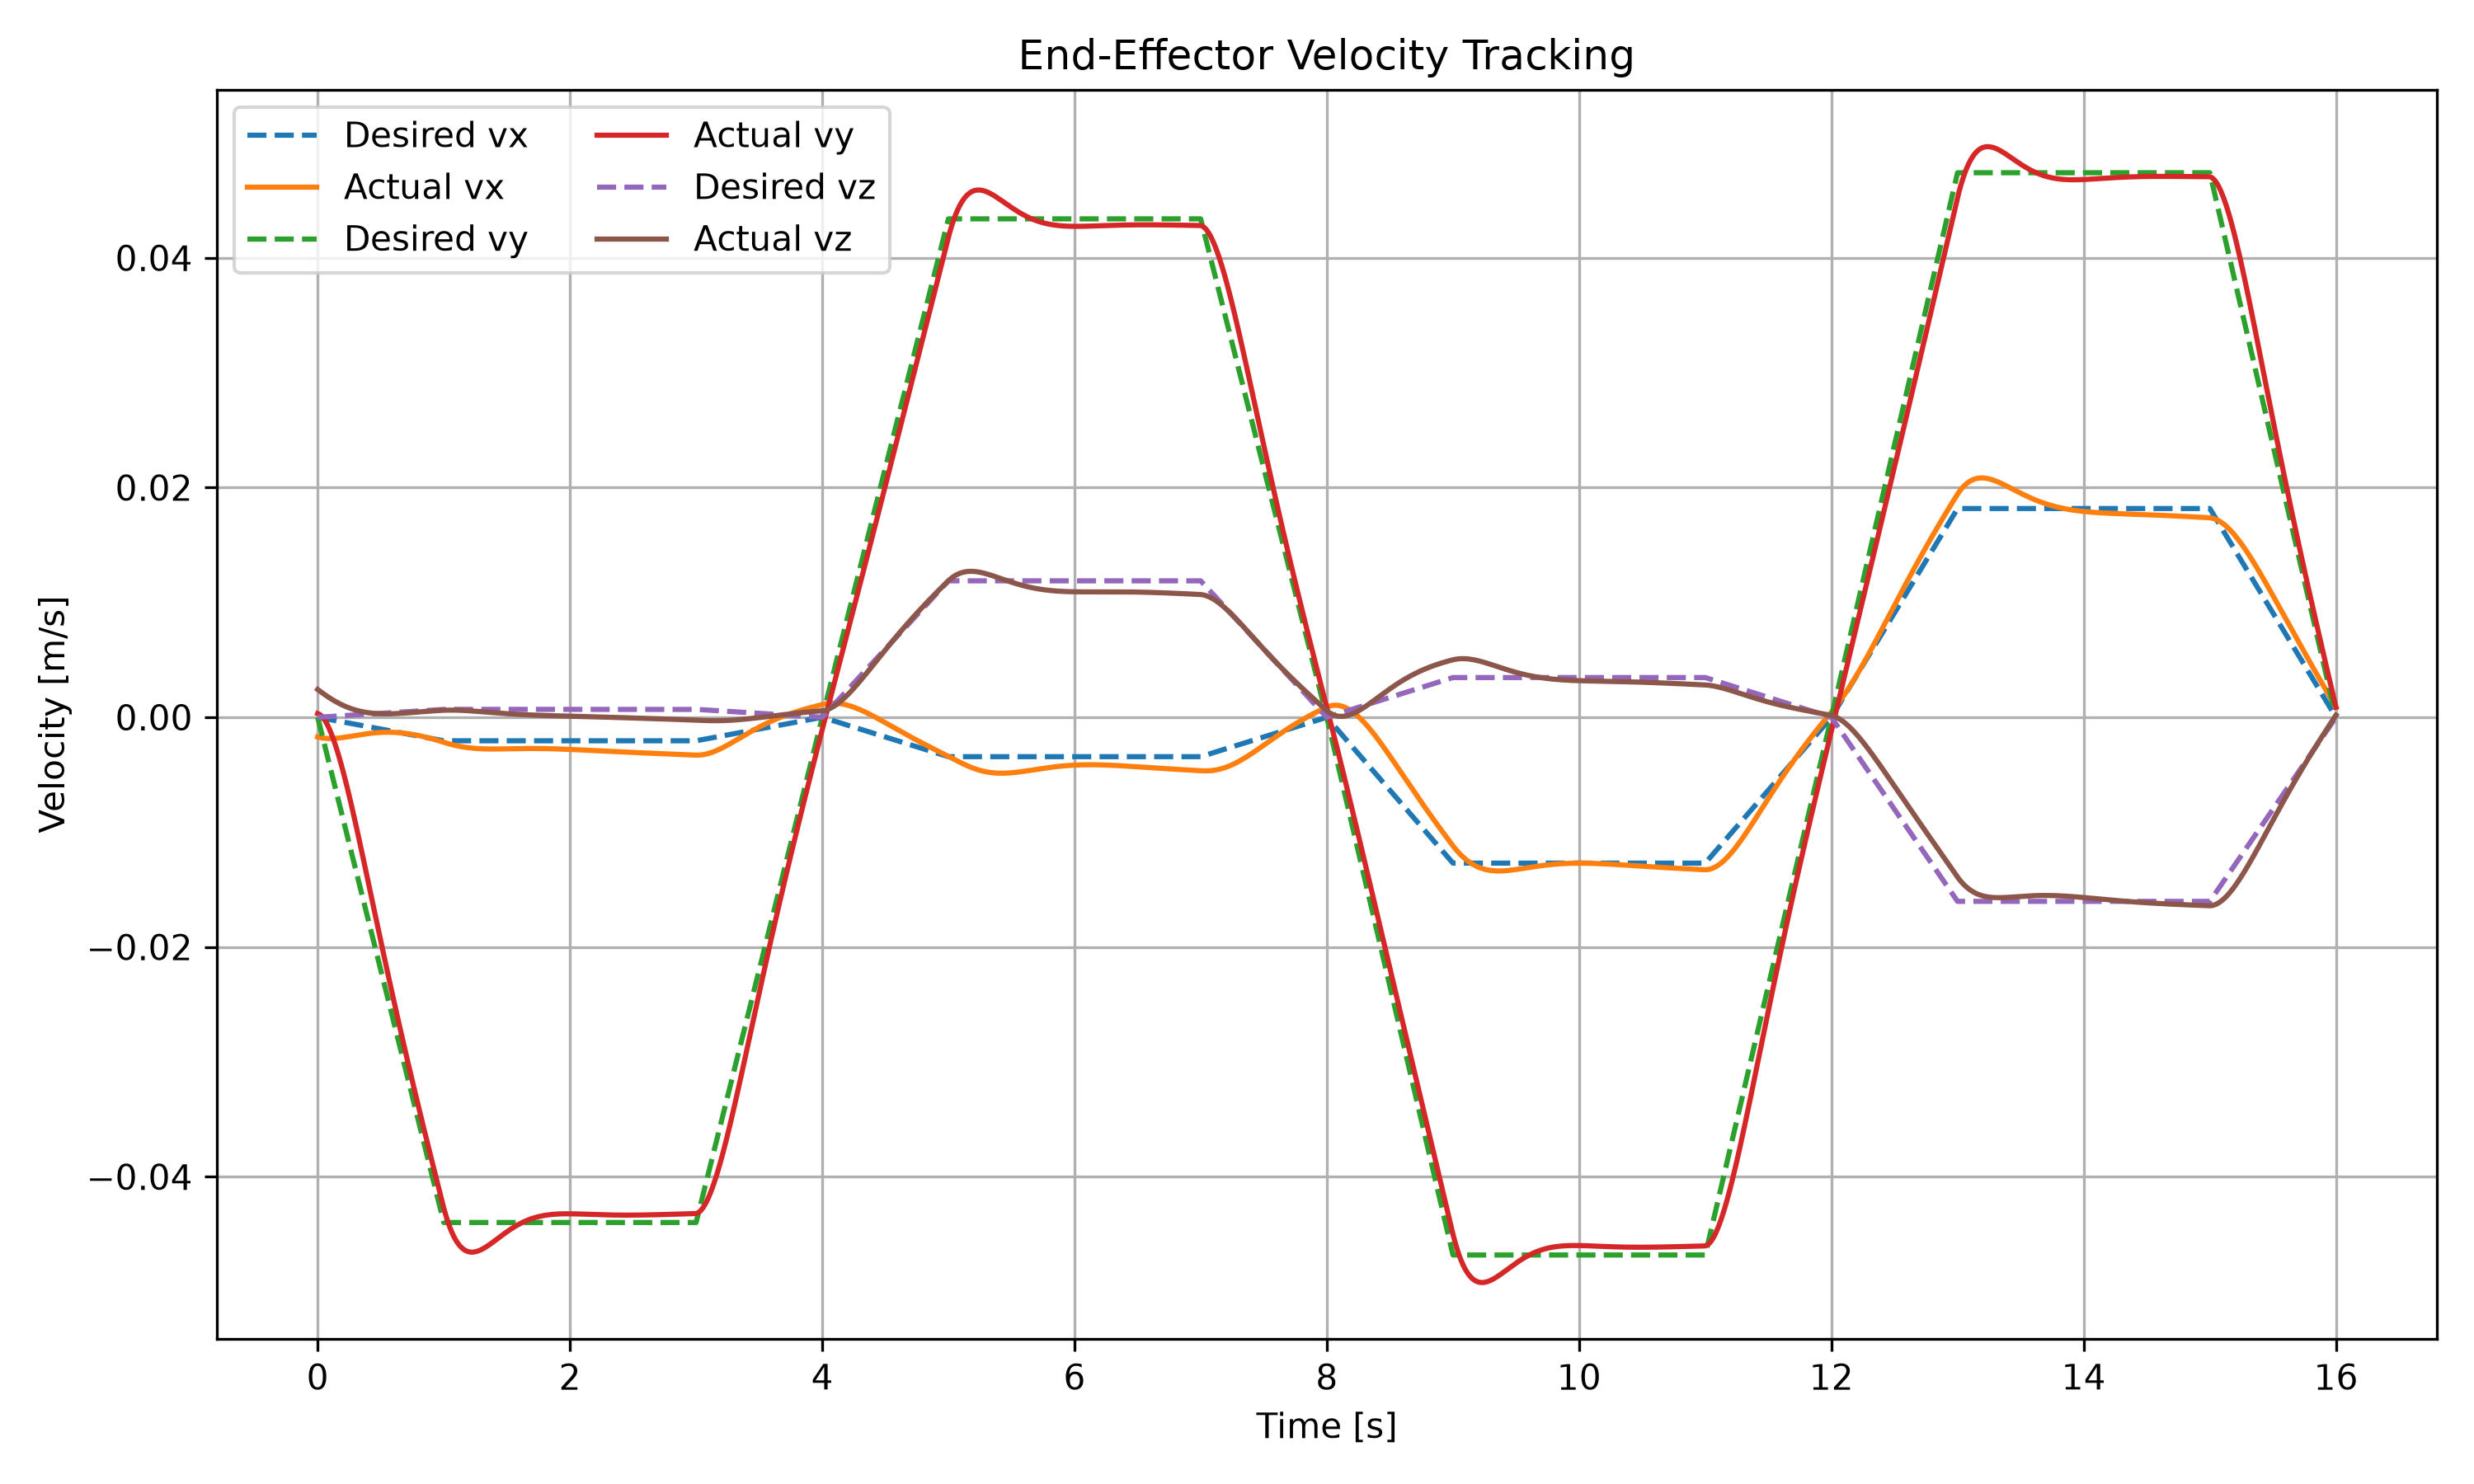
\includegraphics[width=.84\linewidth]{trajectory_velocity_tracking.png}
\caption{Commanded and measured Cartesian velocity in the completed LSPB trial (seed 19).}
\label{fig:lspb-velocity}
\end{figure}
\begin{figure}[!htbp]
\centering
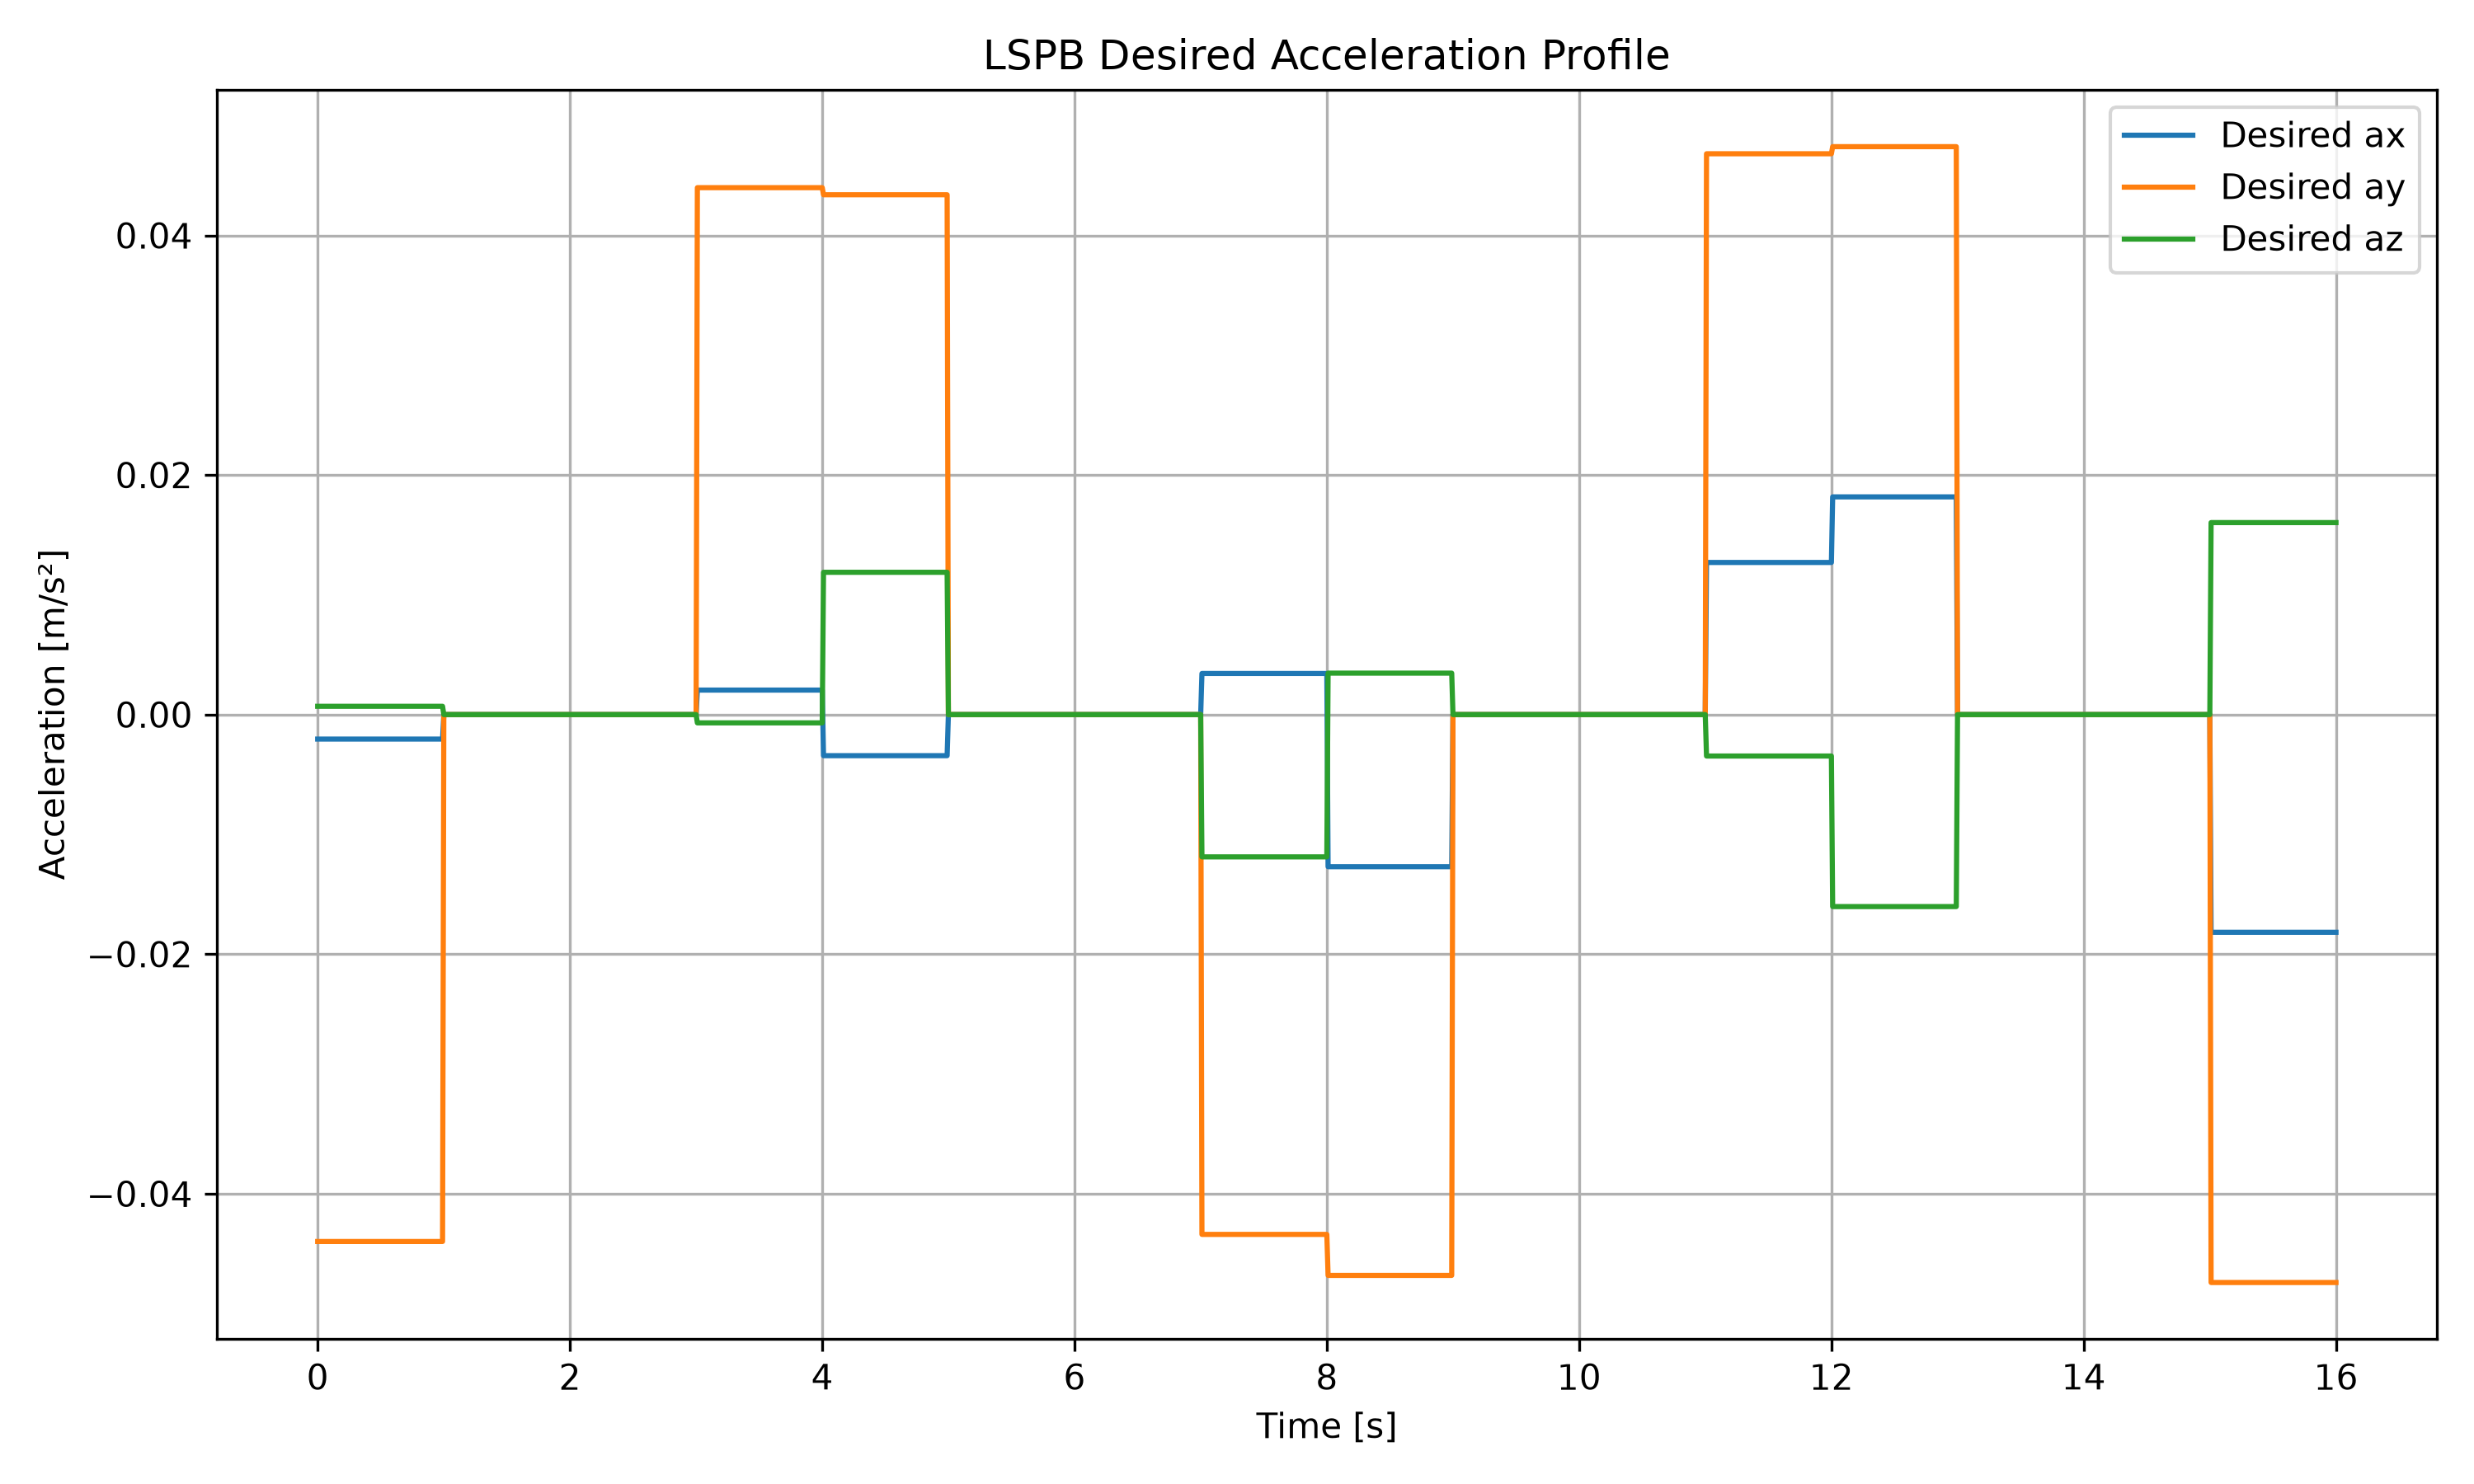
\includegraphics[width=.84\linewidth]{trajectory_acceleration_profile.png}
\caption{Commanded acceleration associated with the parabolic blends in seed 19.}
\label{fig:lspb-acceleration}
\end{figure}
\begin{figure}[!htbp]
\centering
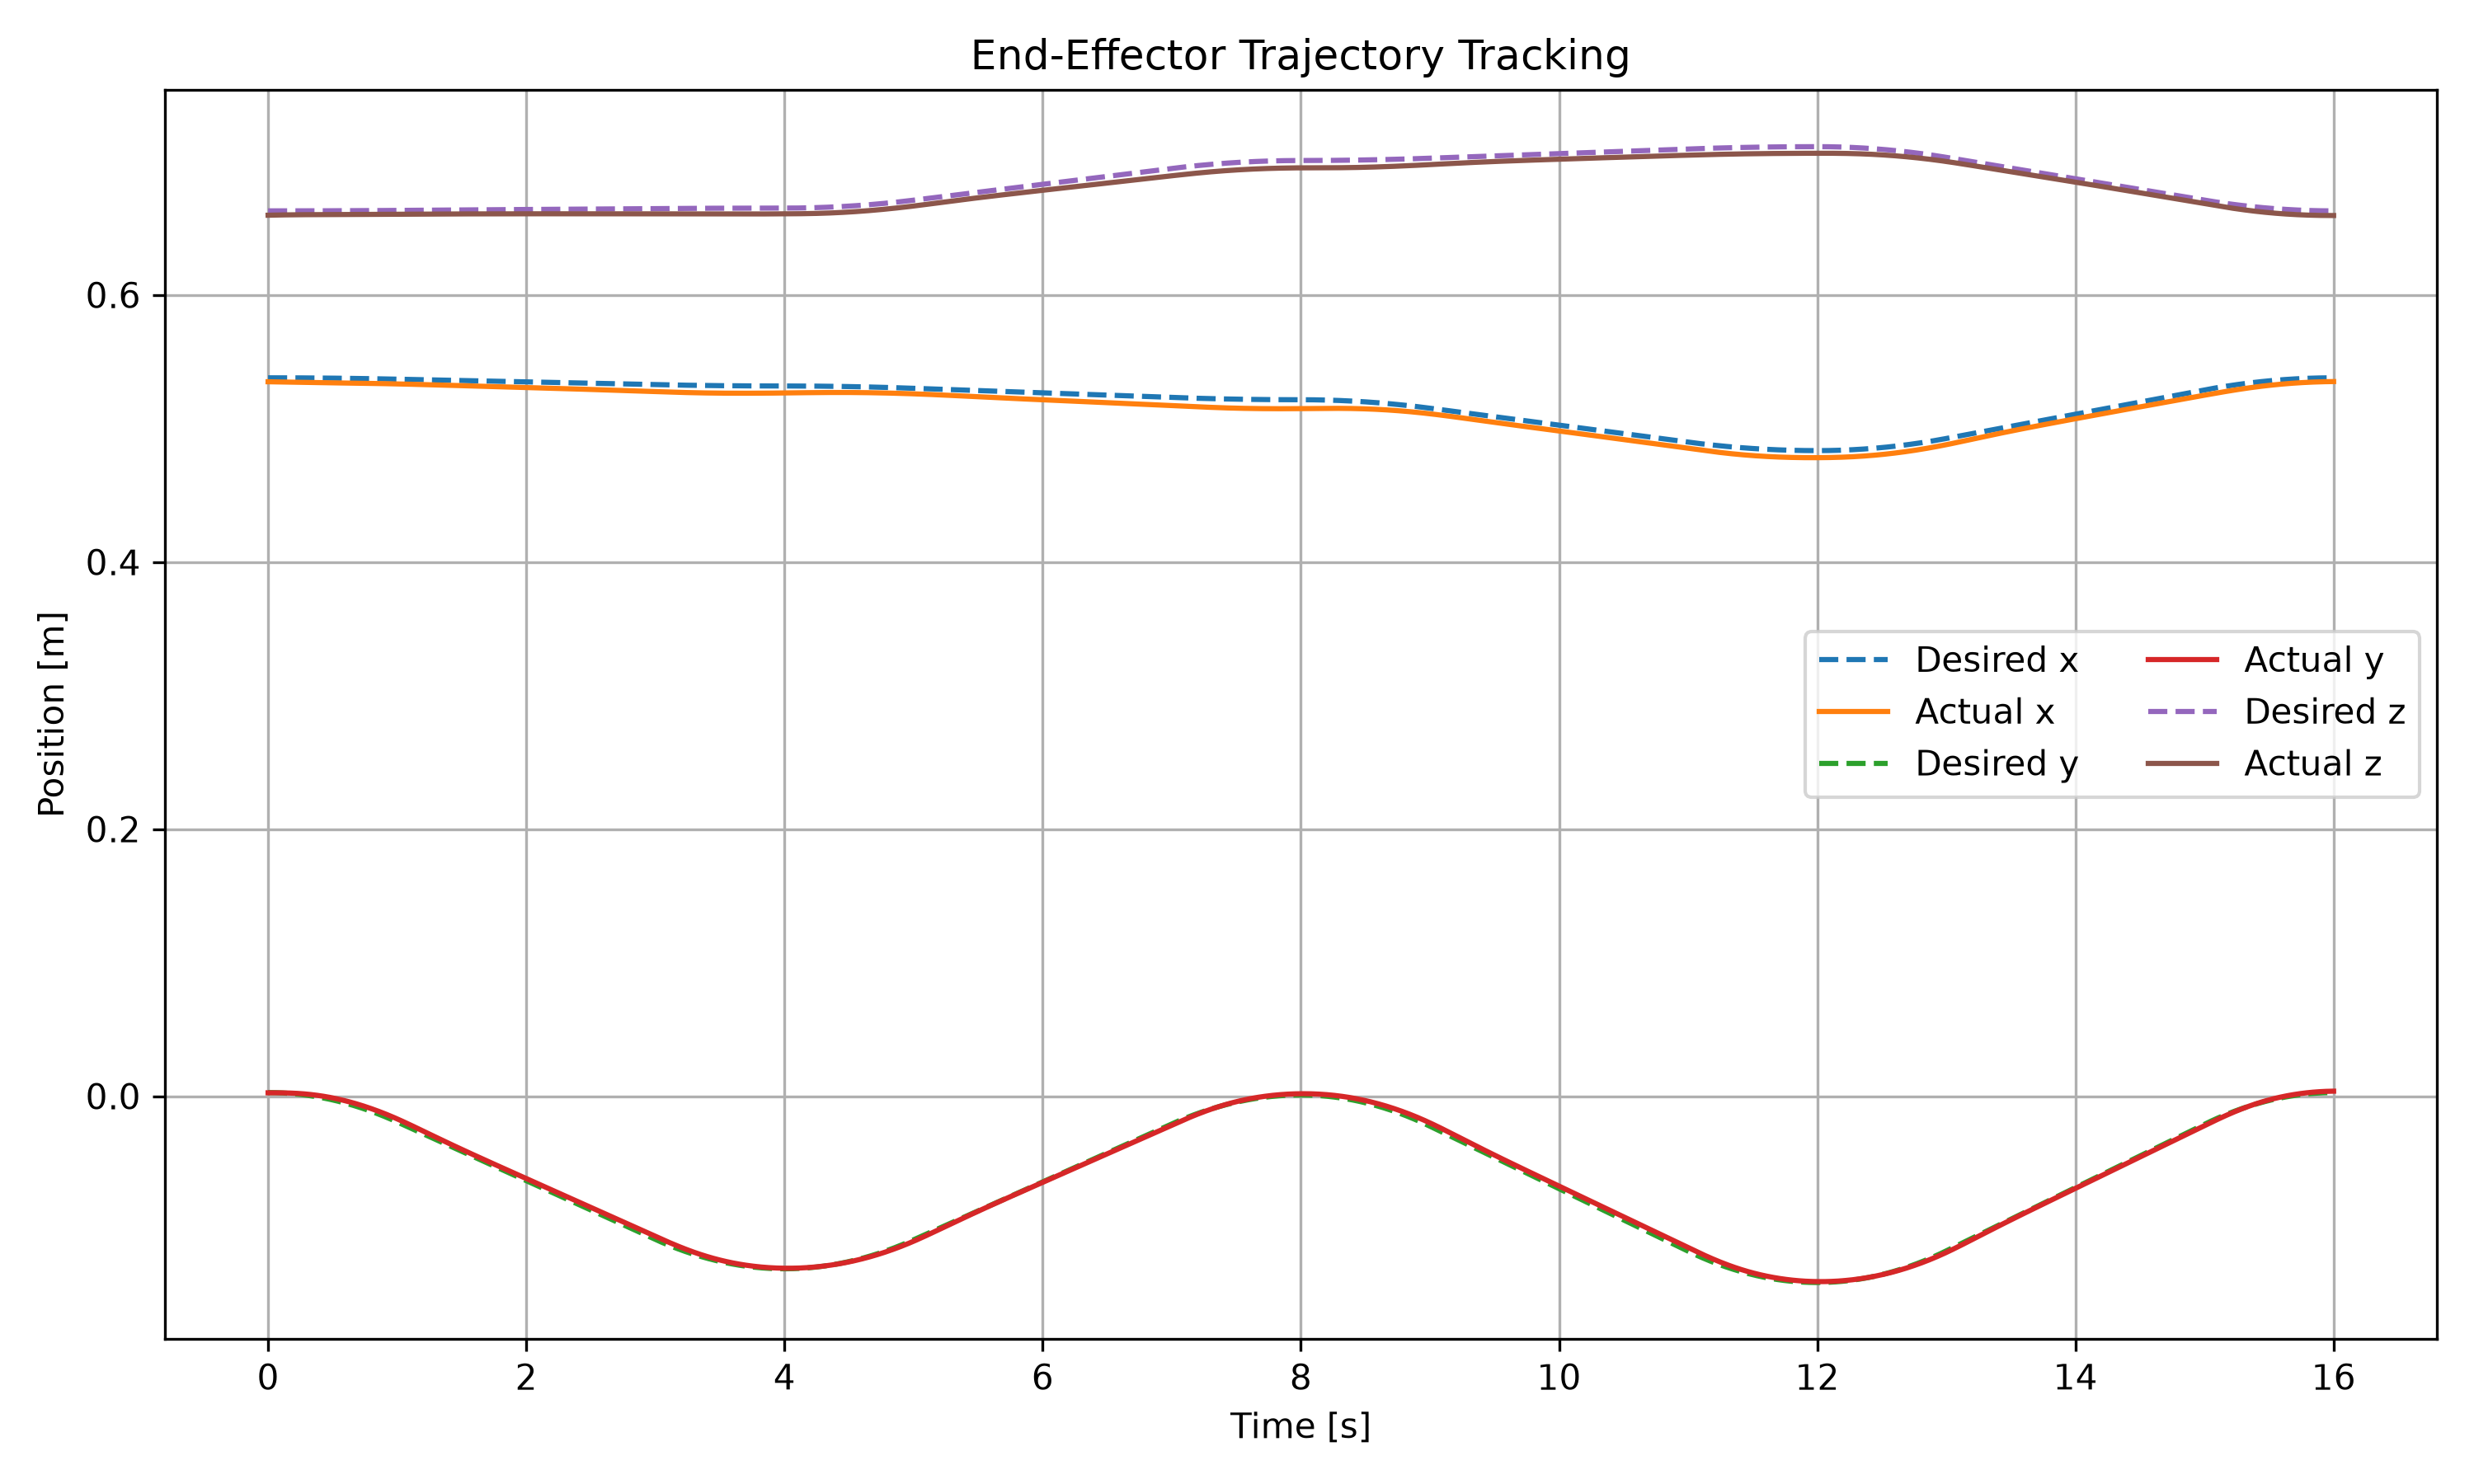
\includegraphics[width=.48\linewidth]{trajectory_position_tracking.png}
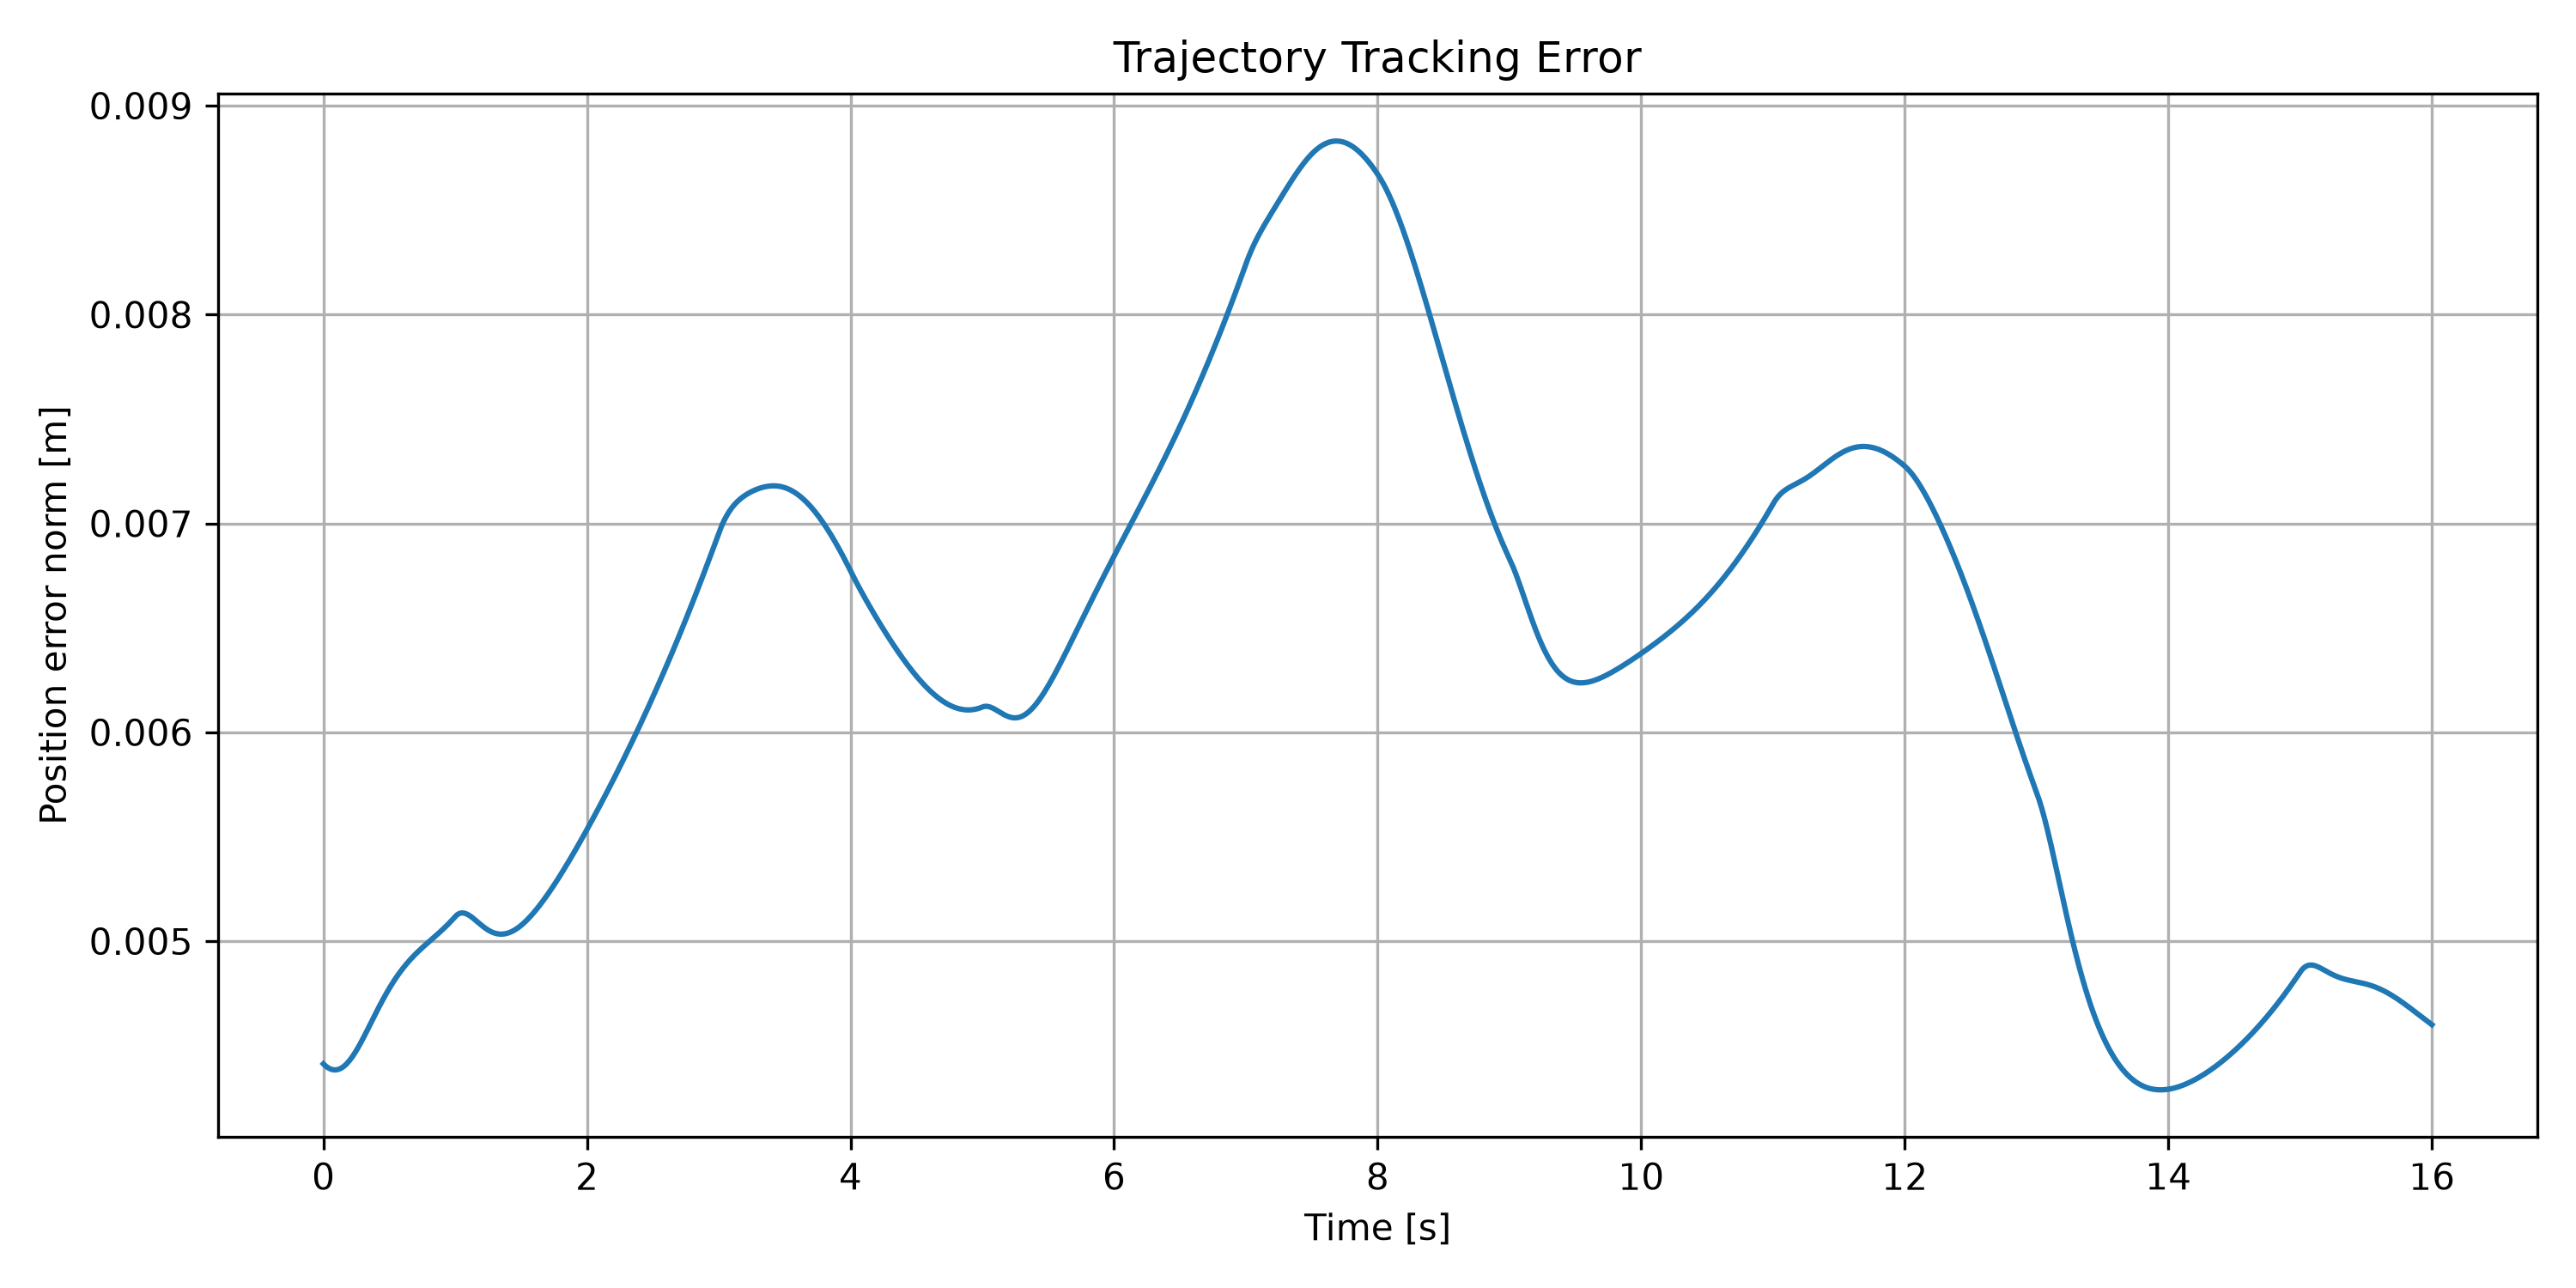
\includegraphics[width=.48\linewidth]{trajectory_position_error.png}
\caption{LSPB seed 19: Cartesian position tracking and Euclidean position error.}
\end{figure}
\begin{figure}[!htbp]
\centering
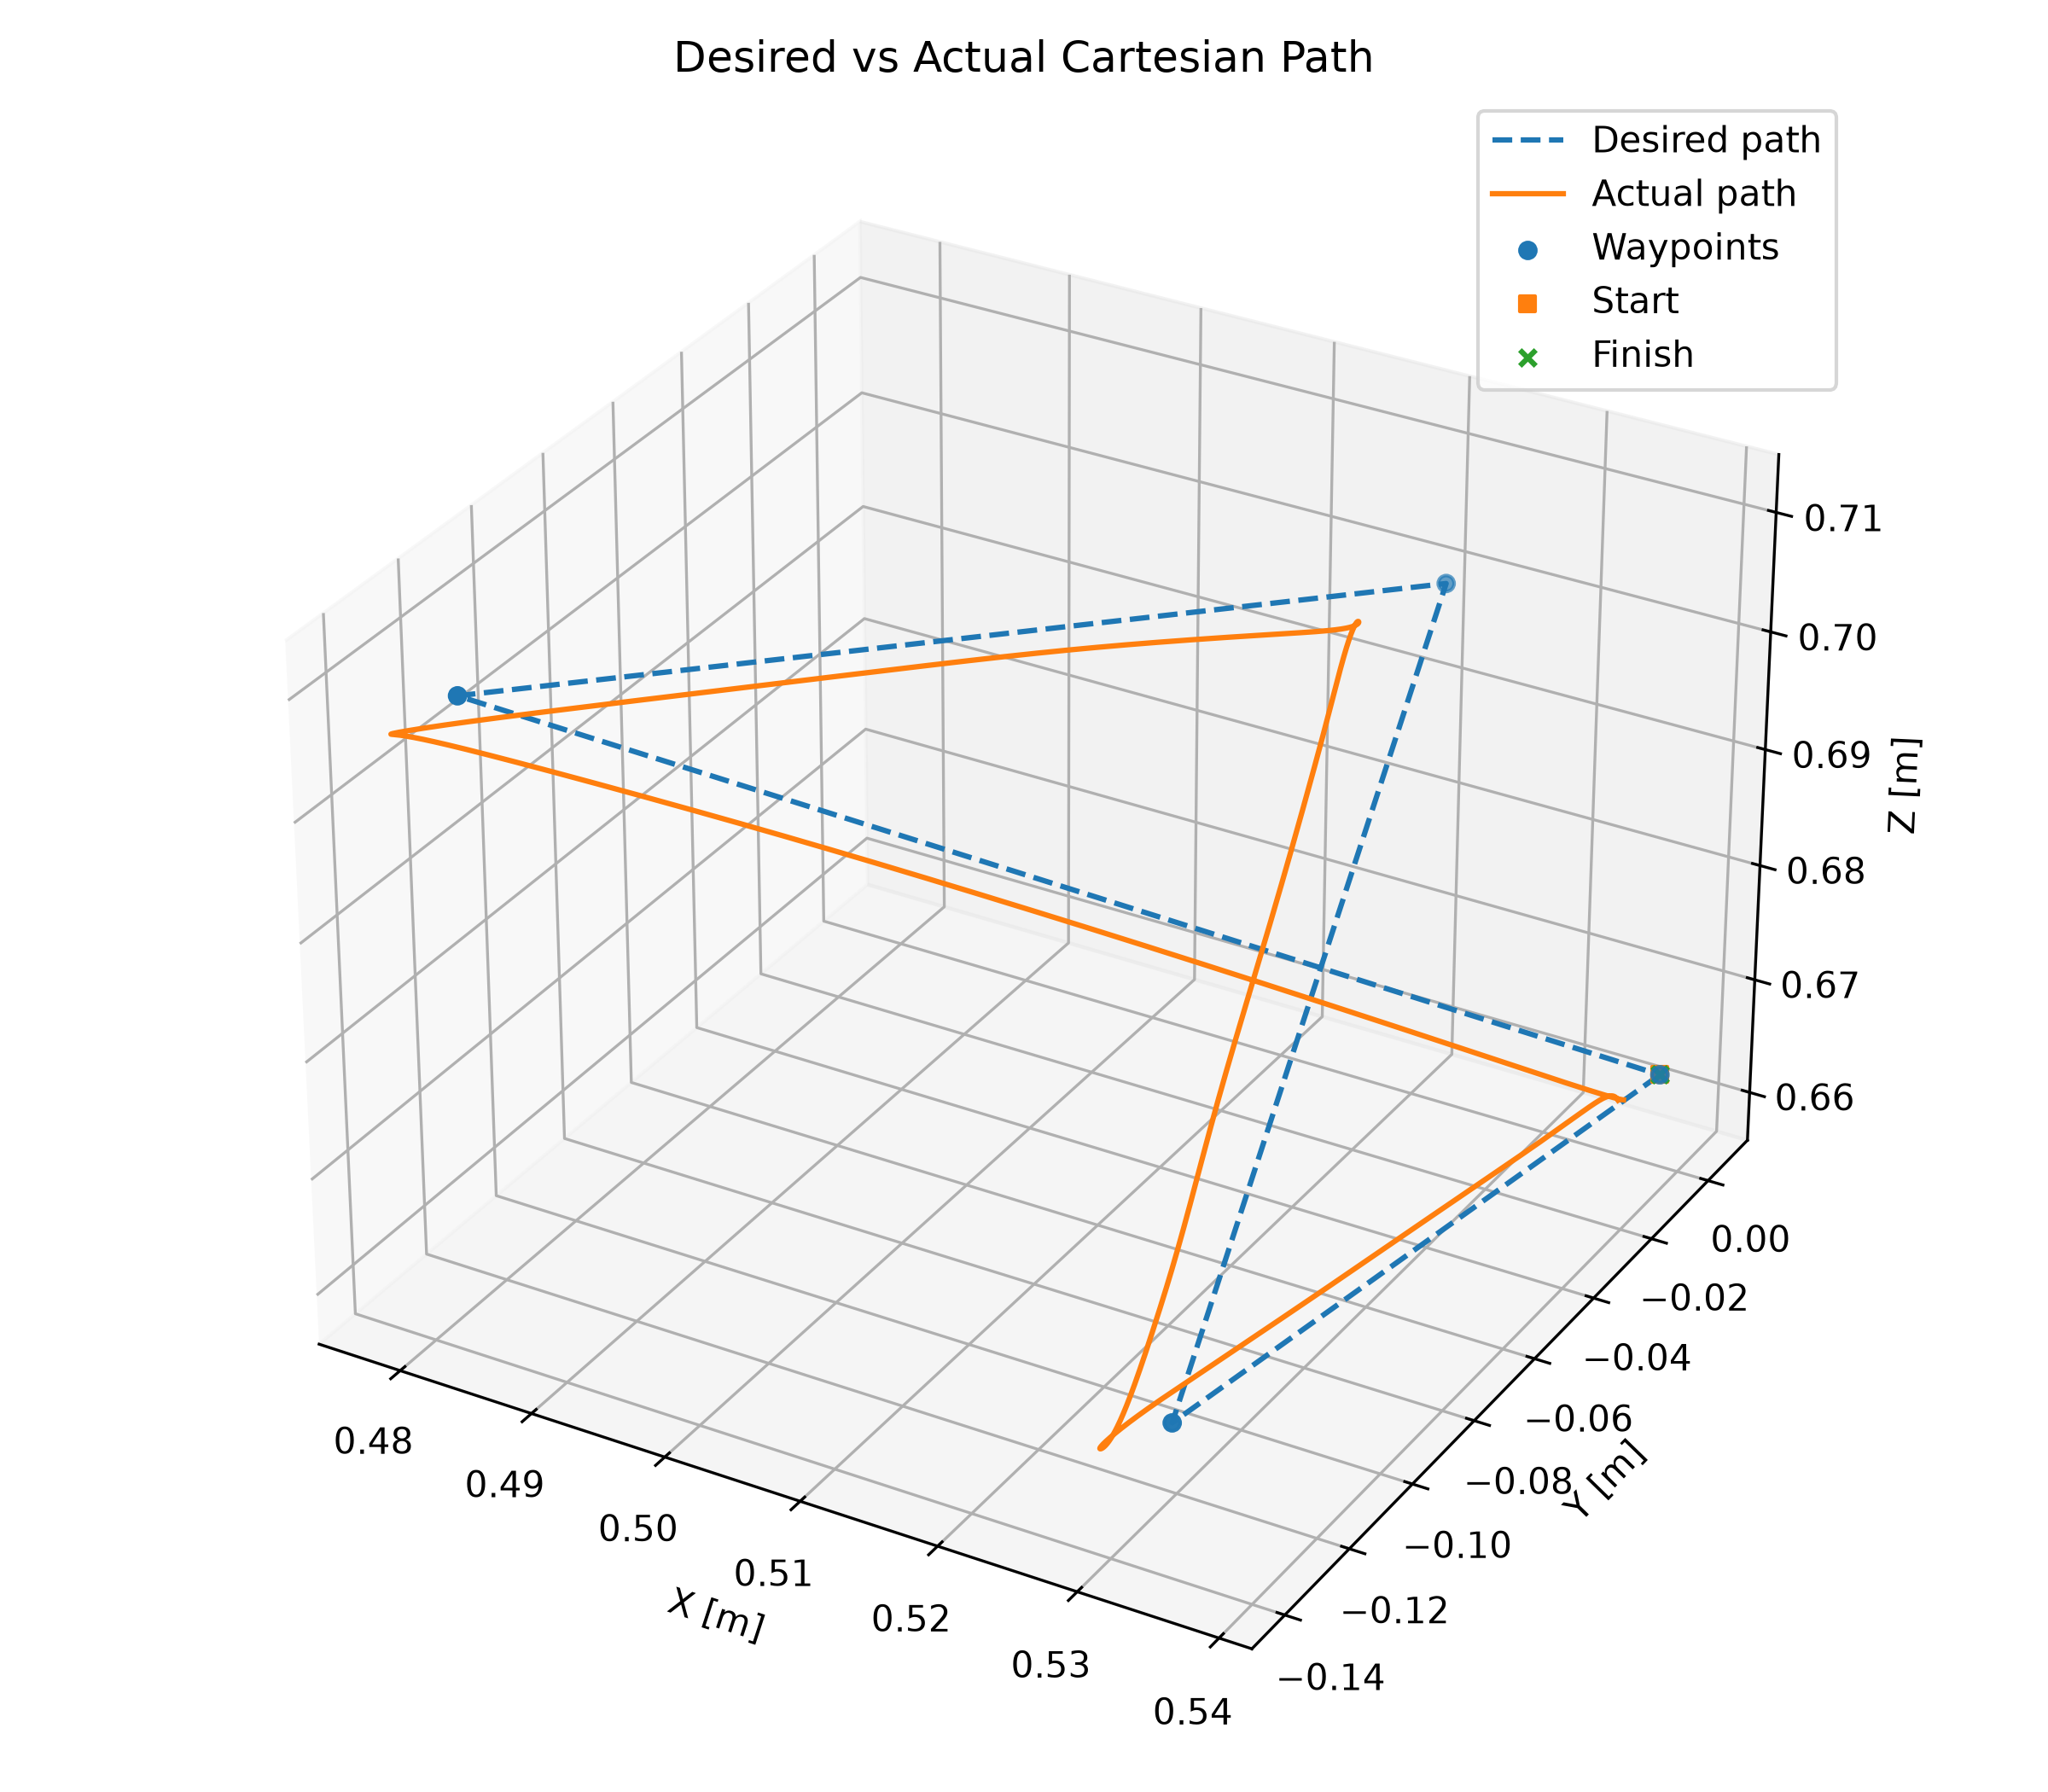
\includegraphics[width=.68\linewidth]{trajectory_3d_path.png}
\caption{LSPB seed 19: commanded and measured three-dimensional paths and waypoints.}
\end{figure}
\section{Cartesian Trajectory Tracking}
Three analytic paths were evaluated: a horizontal ellipse (labelled \texttt{circle} in the logs), a figure-eight with a vertical component, and a two-turn path labelled \texttt{helix} with a sinusoidal height. The ellipse spans 120 mm in $x$ and 320 mm in $y$. The figure-eight spans 120, 160 and 100 mm along $x,y,z$, respectively. The helix spans 120, 280 and 120 mm. These excursions cover lateral motion and height variation above the table. Sixteen representative poses per run were screened with full-pose IK.

The paths are defined analytically about $(0.47,0,0.68)$ m and sampled in equal 10 ms intervals with analytic velocity references. There are no independently sampled waypoints in these trials. With $u=2\pi t/T$ and $T=12$ s, the offsets from the path centre are
\begin{align*}
\bm p_{\rm ellipse} &= (0.06\cos u,\ 0.16\sin u,\ 0),\\
\bm p_{\rm eight} &= (0.06\sin u,\ 0.16\sin u\cos u,\ 0.05\cos u),\\
\bm p_{\rm helix} &= (0.06\cos 2u,\ 0.14\sin 2u,\ 0.06\sin u).
\end{align*}
Each path was run five times. Seeds spawned from base seed 42 independently perturb each home joint by up to 0.04 rad and the path centre by up to 15 mm in $x,y$ and 10 mm in $z$. The controller first settles at the initial path point. The orientation is held at its initial value during each run. Success requires peak Euclidean position error at or below 50 mm. Position RMSE is the square root of the mean squared Euclidean distance over a run. Entries below summarize the per-run metrics as mean $\pm$ sample standard deviation.
\begin{table}[!htbp]
\centering\small
\caption{Trajectory tracking at a 12 s traversal time per trial. Peak errors are maxima within each trial.}
\begin{tabular}{lrrrrr}
\toprule
Path & RMSE (mm) & Peak (mm) & Peak rot. ($^\circ$) & Initial settle (s) & Pass\\
\midrule
Ellipse & $4.86\pm0.11$ & $8.56\pm0.22$ & $0.45\pm0.02$ & $1.33\pm0.07$ & 5/5 (100\%)\\
Figure-eight & $6.43\pm0.14$ & $11.56\pm0.14$ & $0.63\pm0.02$ & $1.49\pm0.08$ & 5/5 (100\%)\\
Helix & $9.87\pm0.46$ & $18.62\pm0.41$ & $0.92\pm0.03$ & $1.09\pm0.40$ & 5/5 (100\%)\\
\bottomrule
\end{tabular}
\end{table}

All 15 runs met the peak-error criterion, with zero sampled torque clipping. The helix had the largest tracking error. Its two planar turns in the same traversal time increase reference speed and acceleration, while its height variation changes the operating configuration.
\begin{figure}[!htbp]
\centering
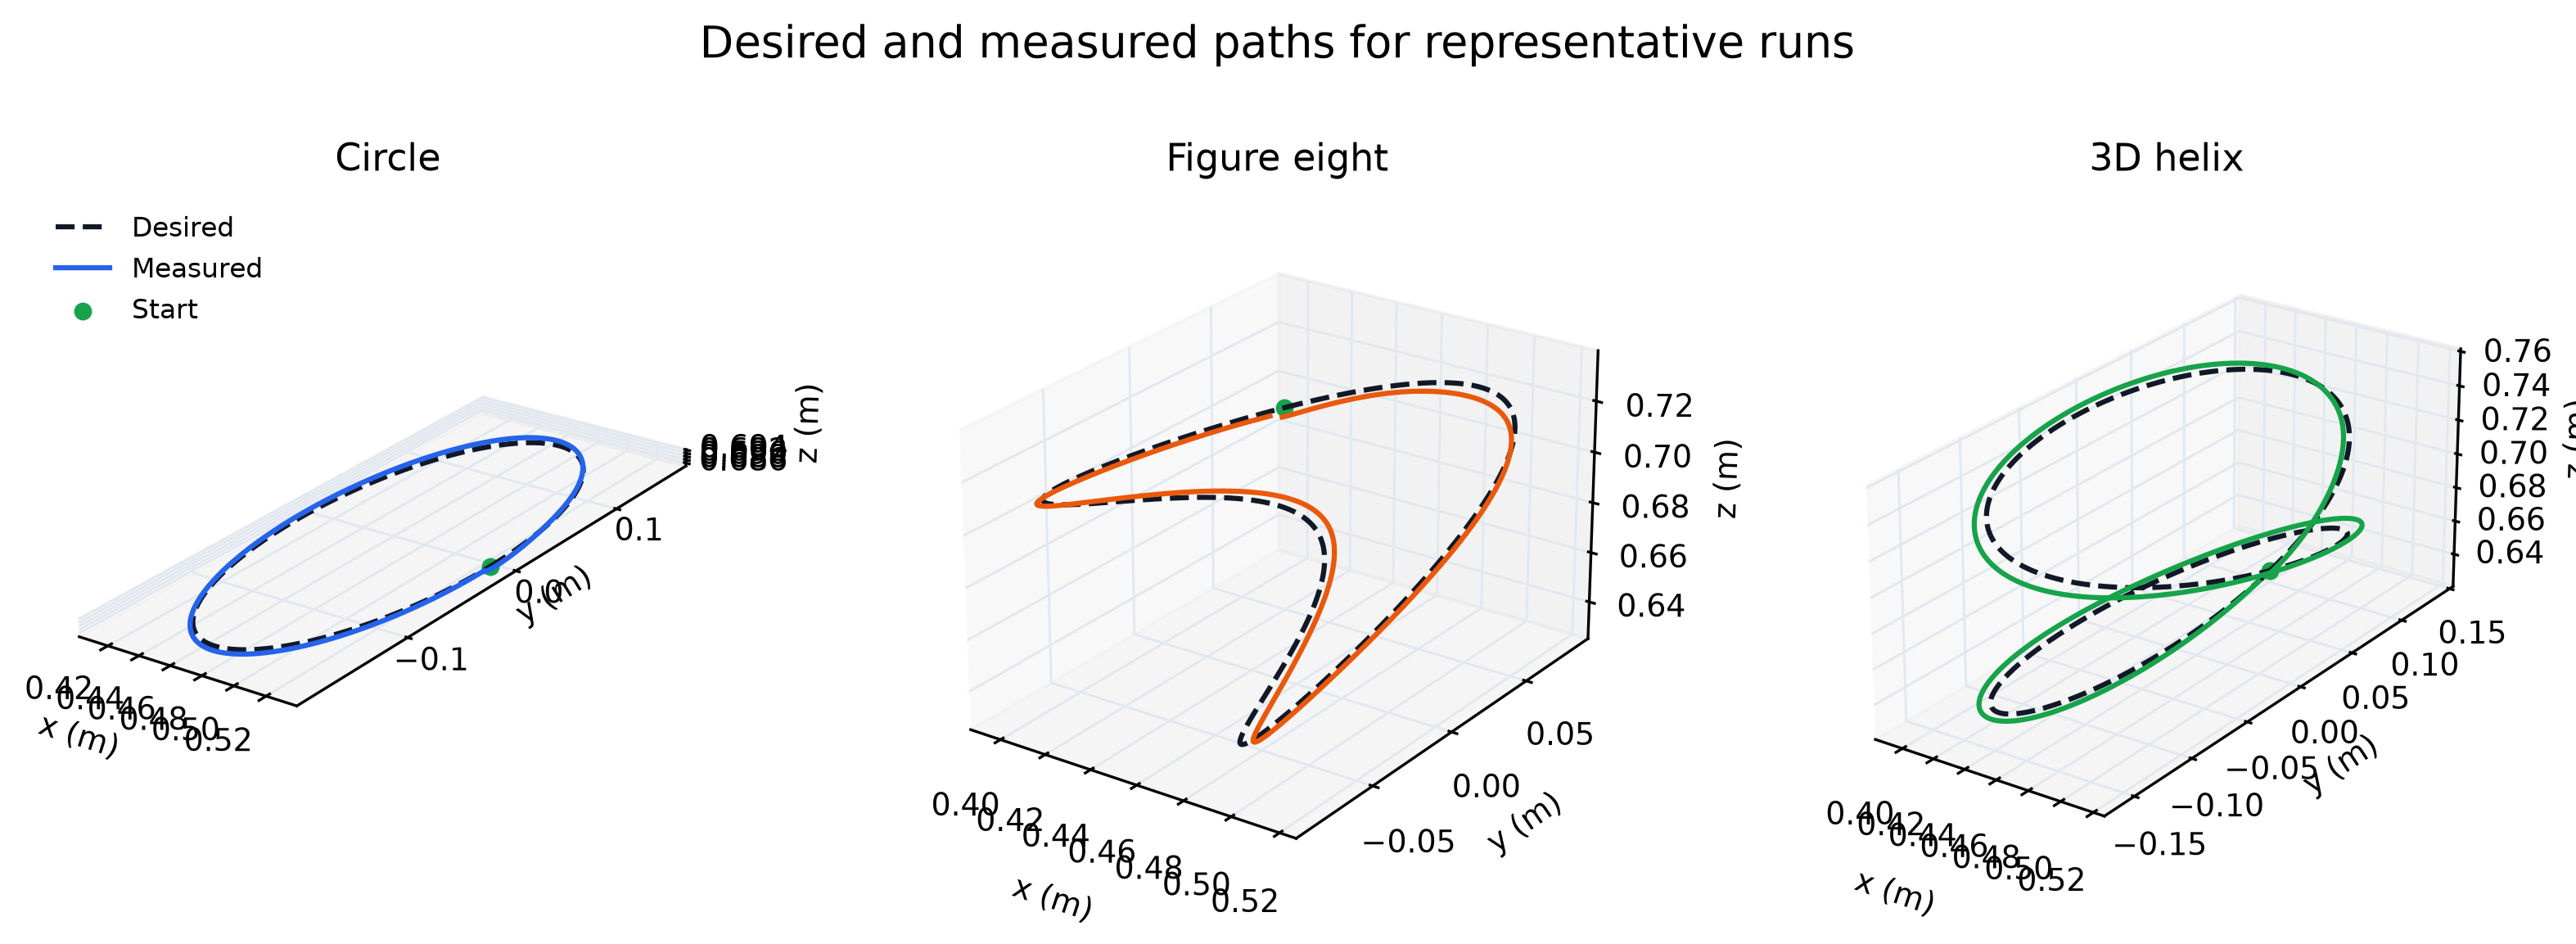
\includegraphics[width=.99\linewidth]{trajectory_path_comparison.png}
\caption{Desired and measured paths for representative trials of each trajectory.}
\end{figure}
Figure~\ref{fig:figure-eight-video} shows the Panda and the commanded path in a representative viewer run. The log-derived sequence that follows gives the simulated timing and measured hand trace for the first recorded figure-eight trial.

\begin{figure}[!htbp]
\centering
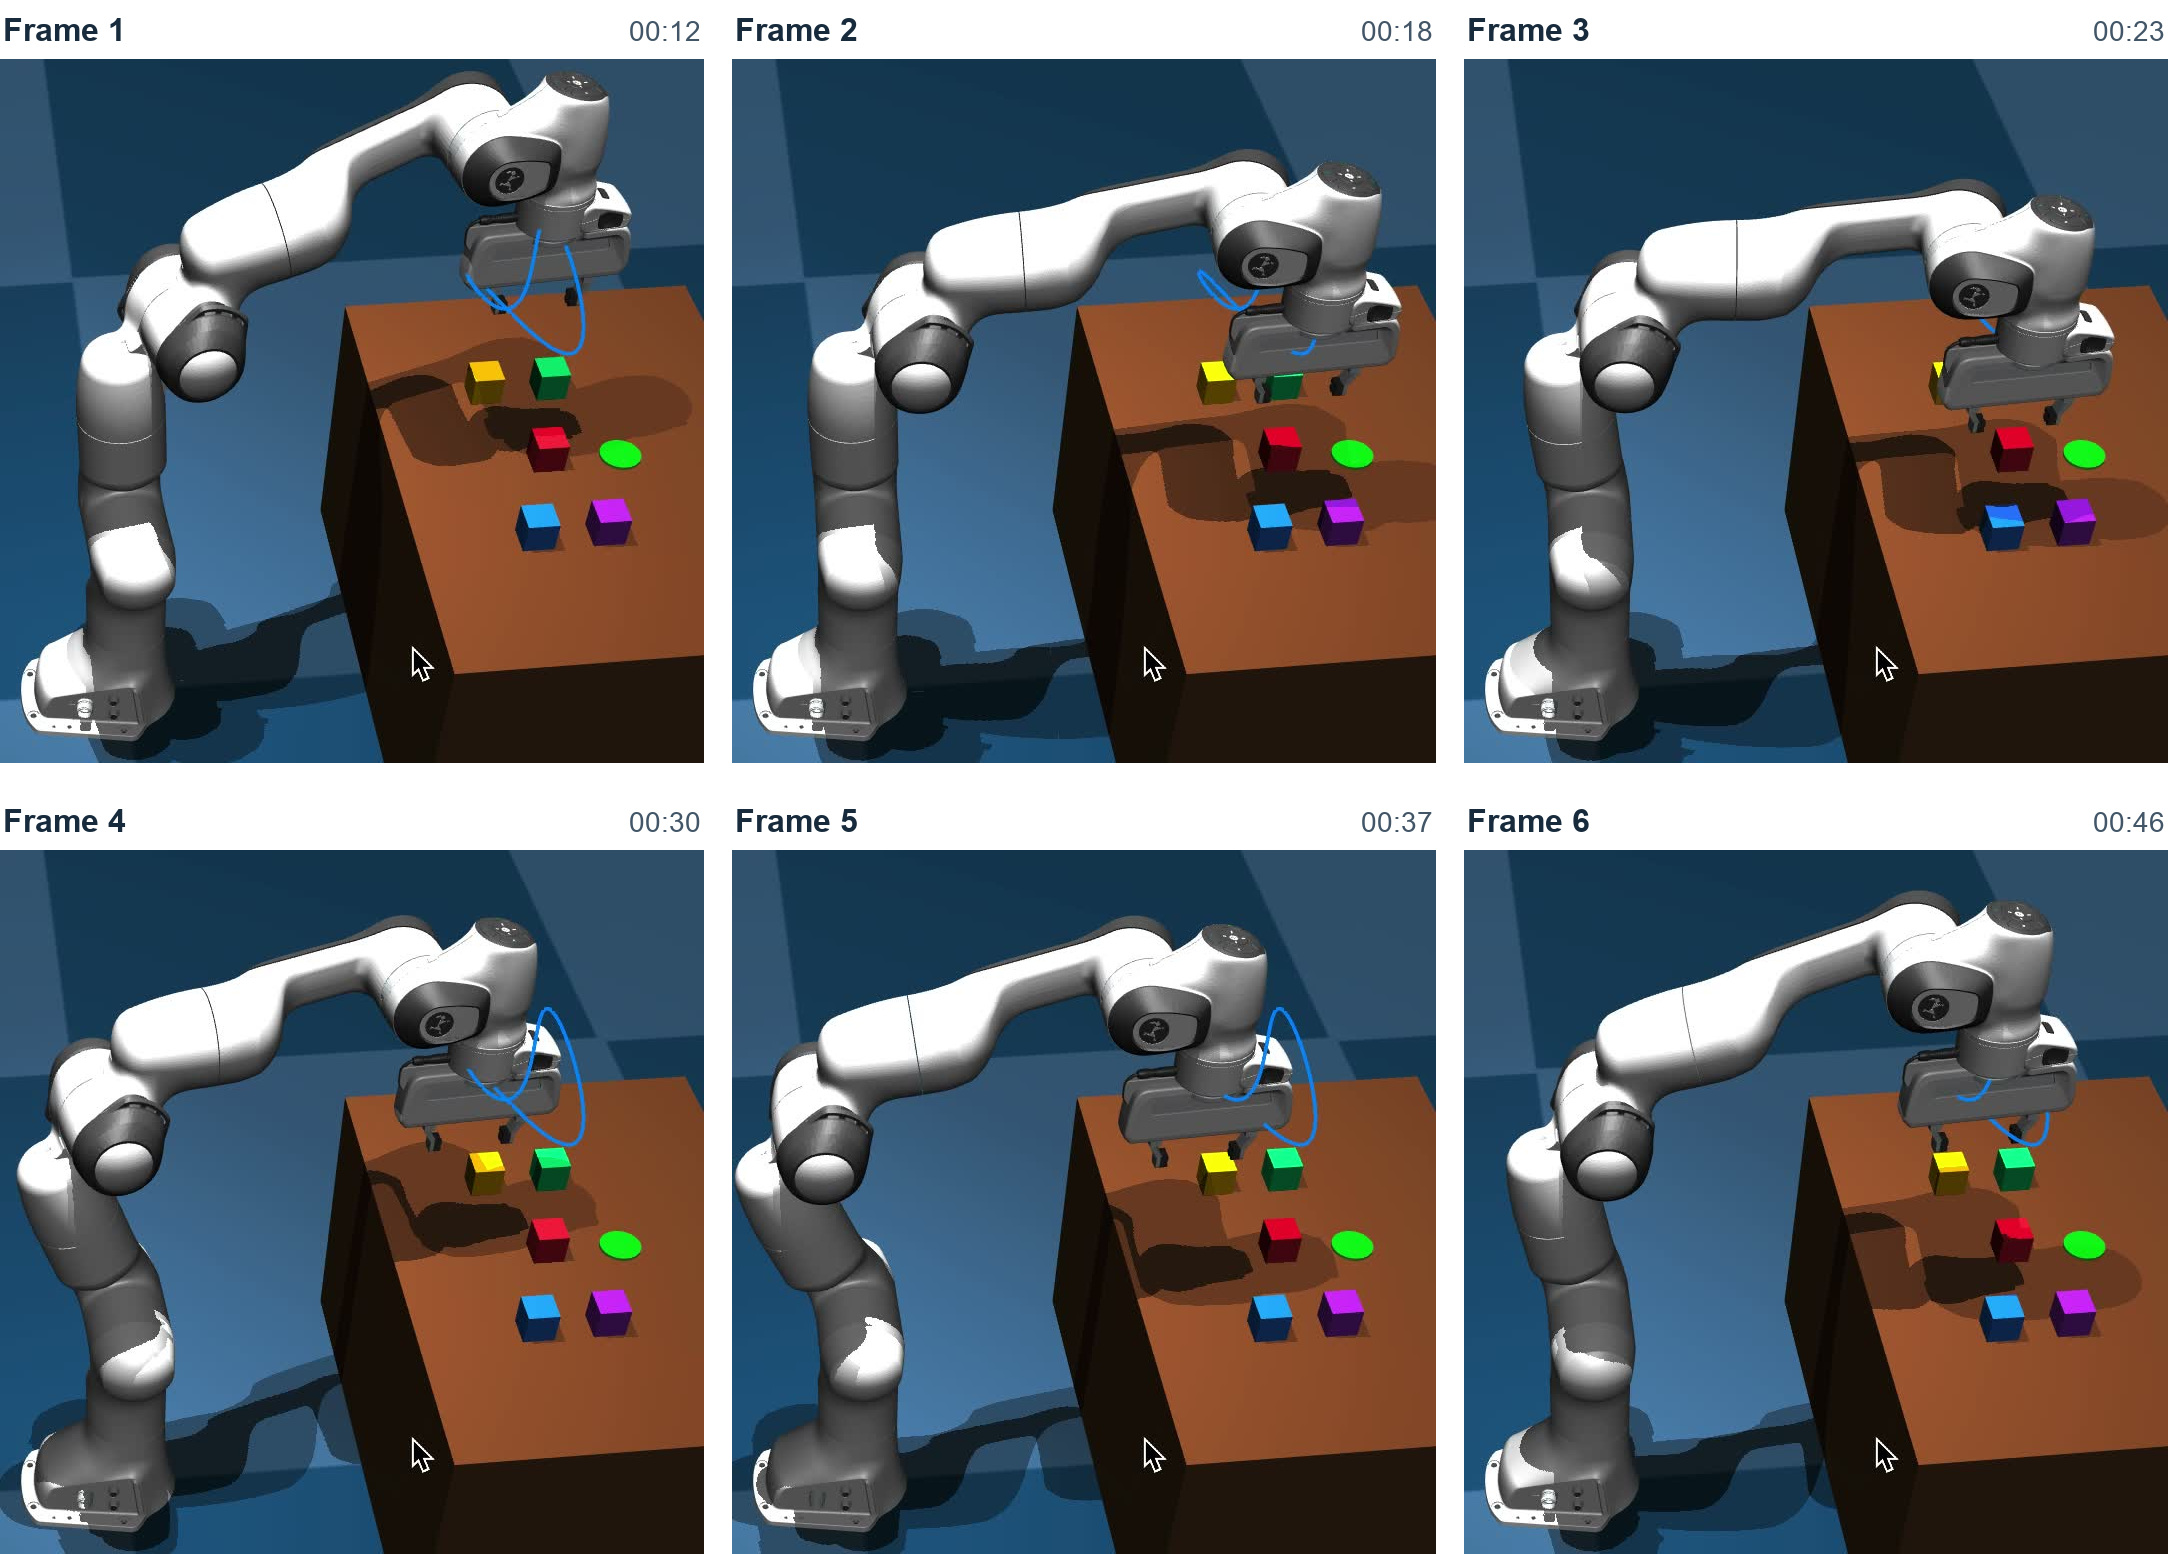
\includegraphics[width=.96\linewidth]{figure_eight_video_frames.jpg}
\caption{Six chronological MuJoCo screen-recording frames from the figure-eight viewer run (base seed 42, path centre height 0.68 m). The blue line shows the commanded path as the hand moves across the workspace. Read the panels left to right, top row first. Timestamps refer to video playback.}
\label{fig:figure-eight-video}
\end{figure}

\begin{figure}[!htbp]
\centering
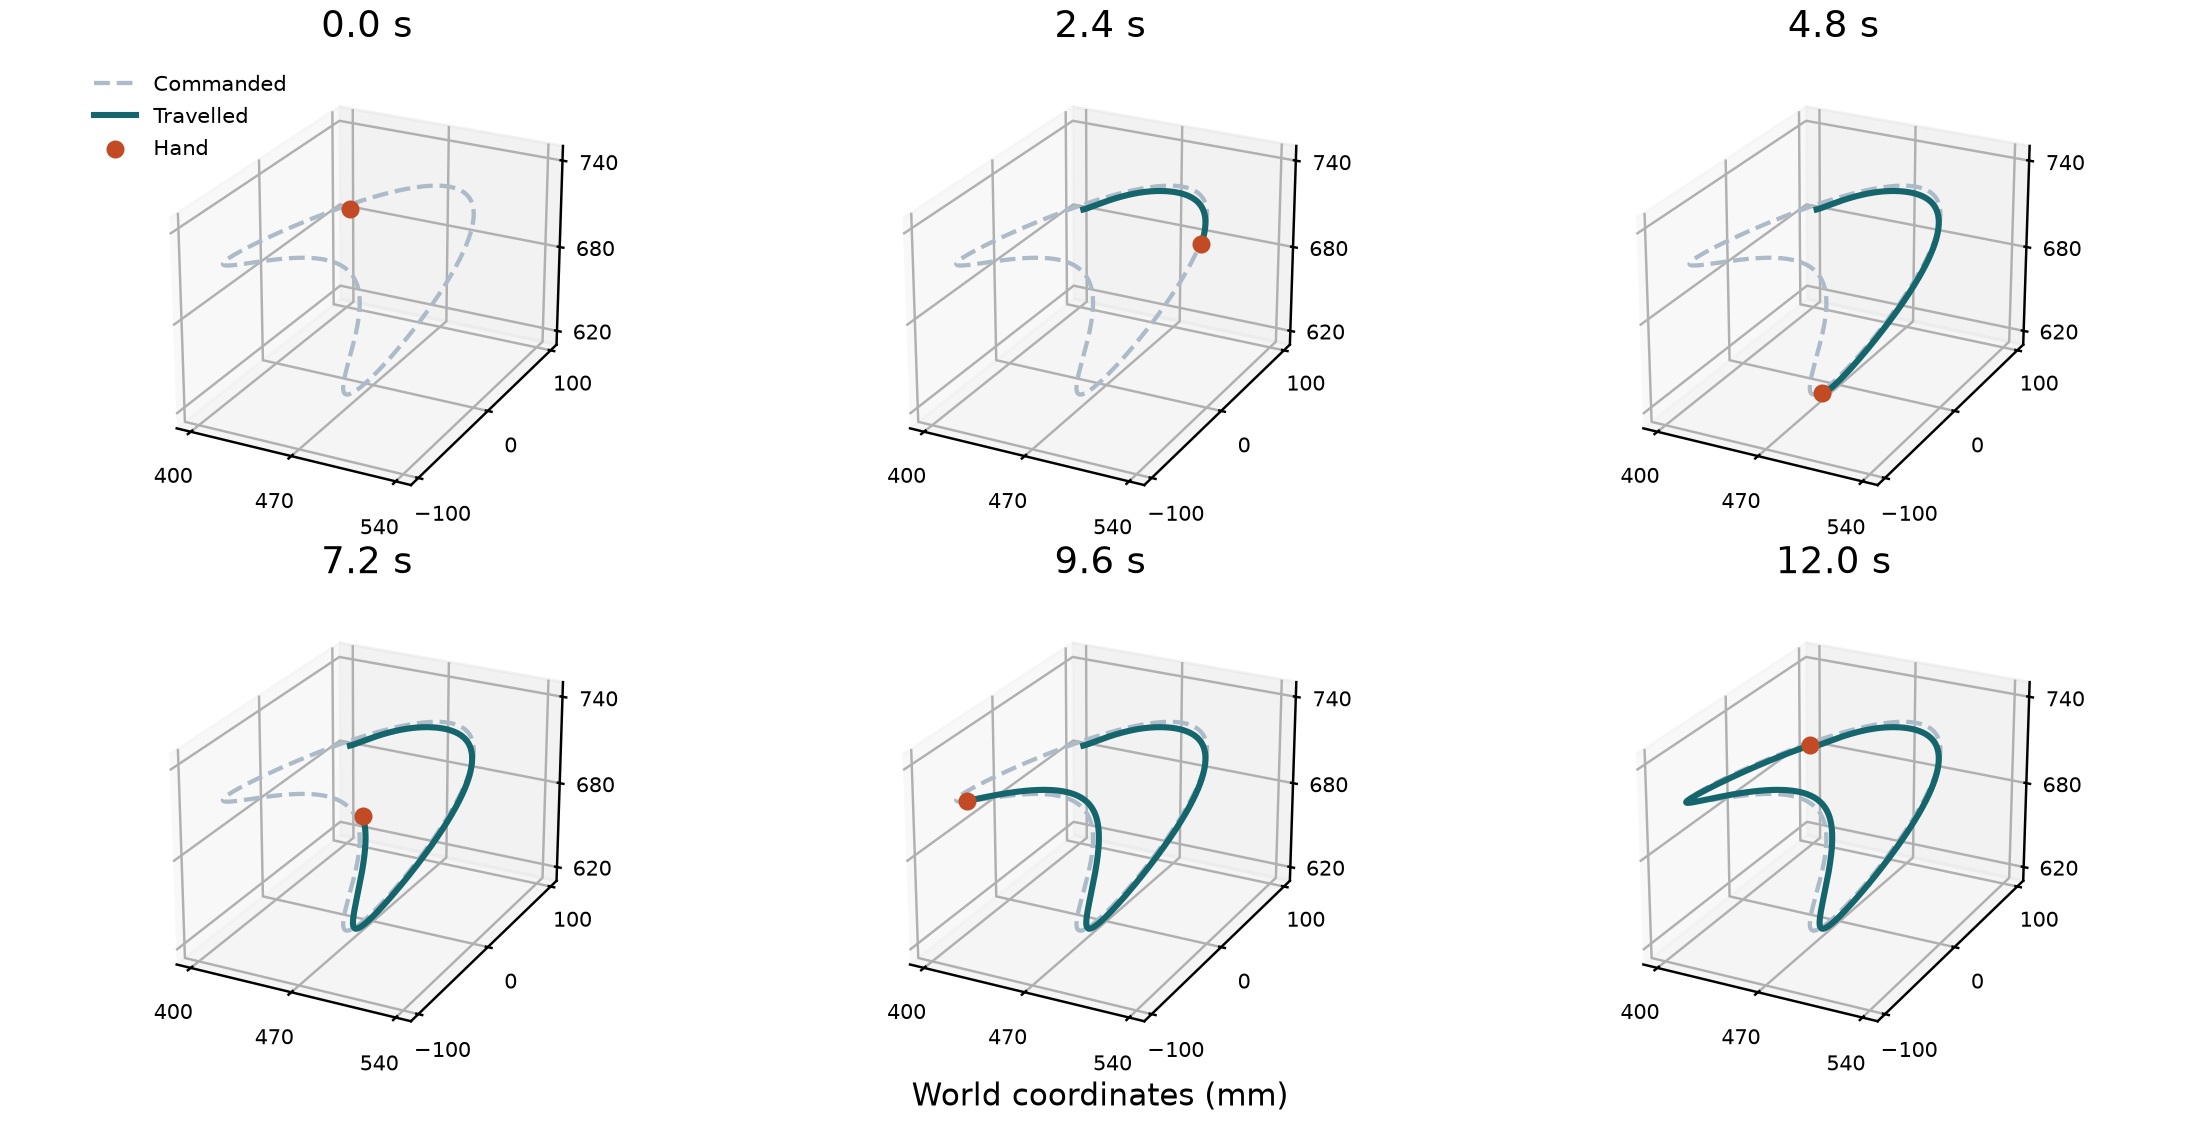
\includegraphics[width=.95\linewidth]{trajectory_sequence.png}
\caption{Figure-eight run 1 at successive times. Each panel shows the logged hand position, its travelled trace, and the full commanded path. The panels use the same projection.}
\end{figure}

\begin{figure}[!htbp]
\centering
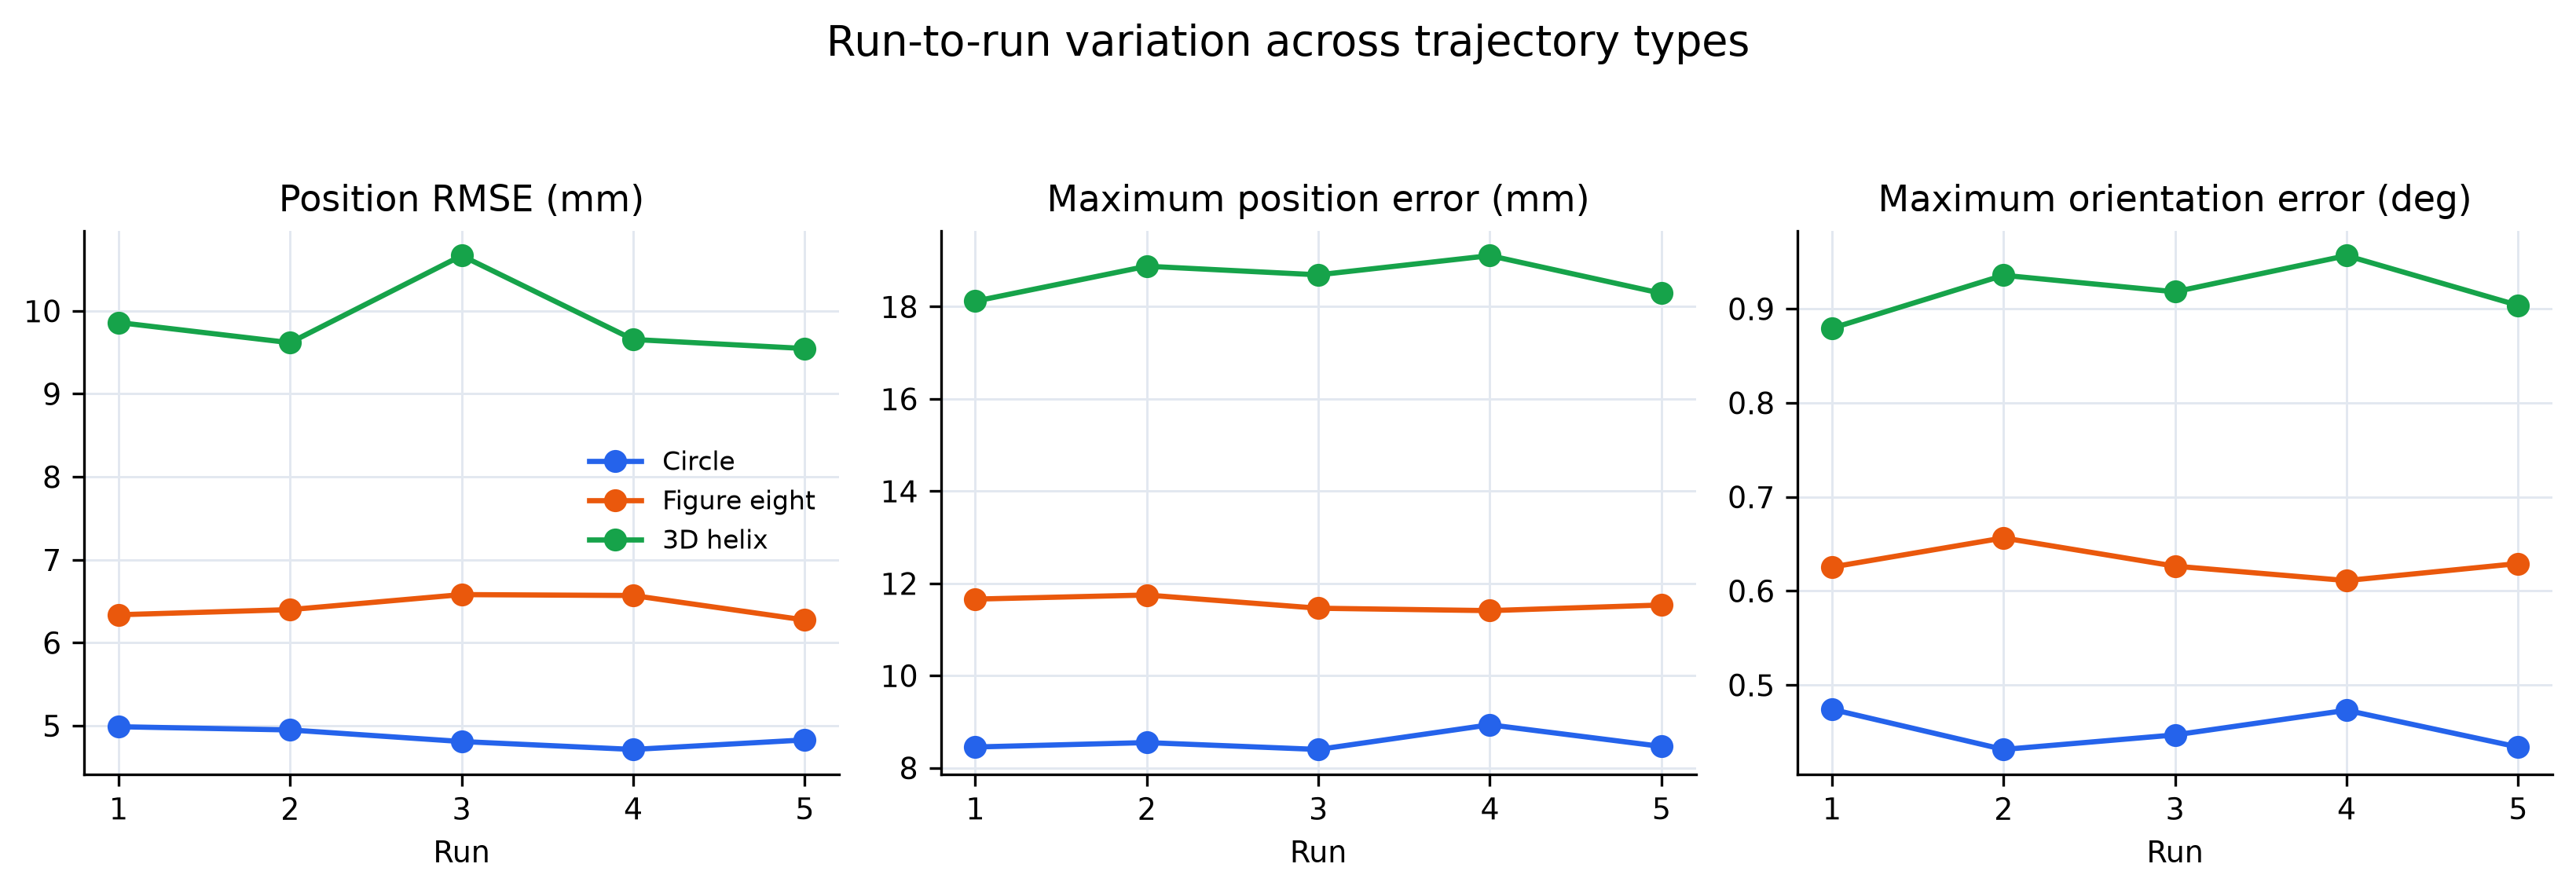
\includegraphics[width=.94\linewidth]{trajectory_run_comparison.png}
\caption{Position error by trial for each path family. The separation between the paths persists across all five trial indices.}
\label{fig:trajectory-trials}
\end{figure}

\section{Controller Performance and Limits}
\subsection{Step response}
Five seeded trials per magnitude, with home-joint perturbations of up to 0.025 rad, applied a $+y$ position step or a world-$z$ orientation step from a hold at $(0.47,0,0.68)$ m. Each response was sampled for 5 s. Rise time measures the 10--90\% interval. Overshoot is the greatest excursion past the target divided by step magnitude. Settling is the first sample after which the response stays inside its band through the end of the trial. The band is 2\% of the step or the code's minimum tolerance, whichever is larger. The script uses a 0.001 SI-unit floor for step magnitudes below 0.2 and a 0.5-degree floor otherwise. The final 0.5 s provides the mean absolute residual.
\begin{table}[!htbp]
\centering\small
\caption{Step response ($n=5$ per condition). Residual units match the step input.}
\begin{tabular}{lrrrrr}
\toprule
Step & Rise (s) & Overshoot (\%) & Settle (s) & Residual & Clipping (\%)\\
\midrule
20 mm & $0.362\pm0.004$ & $6.26\pm0.15$ & $0.878\pm0.008$ & $0.028\pm0.030$ & $0.0\pm0.0$\\
50 mm & $0.360\pm0.000$ & $6.21\pm0.06$ & $1.062\pm0.004$ & $0.039\pm0.034$ & $0.0\pm0.0$\\
100 mm & $0.360\pm0.000$ & $5.80\pm0.08$ & $1.048\pm0.008$ & $0.057\pm0.057$ & $0.0\pm0.0$\\
$5^\circ$ & $0.872\pm0.004$ & $0.00\pm0.00$ & $1.584\pm0.017$ & $0.013\pm0.004$ & $0.0\pm0.0$\\
$15^\circ$ & $0.870\pm0.000$ & $0.00\pm0.00$ & $1.362\pm0.004$ & $0.033\pm0.003$ & $0.0\pm0.0$\\
$30^\circ$ & $0.880\pm0.000$ & $0.00\pm0.00$ & $1.590\pm0.000$ & $0.066\pm0.002$ & $0.2\pm0.0$\\
\bottomrule
\end{tabular}
\end{table}

Position overshoot remained near 6\%. Rotation rose more slowly and had zero measured overshoot. The 30-degree step was the only condition with sampled torque clipping. The step tests characterize the transient response at the tested posture. Closed-loop bandwidth was not measured directly because the study did not include a frequency sweep.

\begin{figure}[!htbp]
\centering
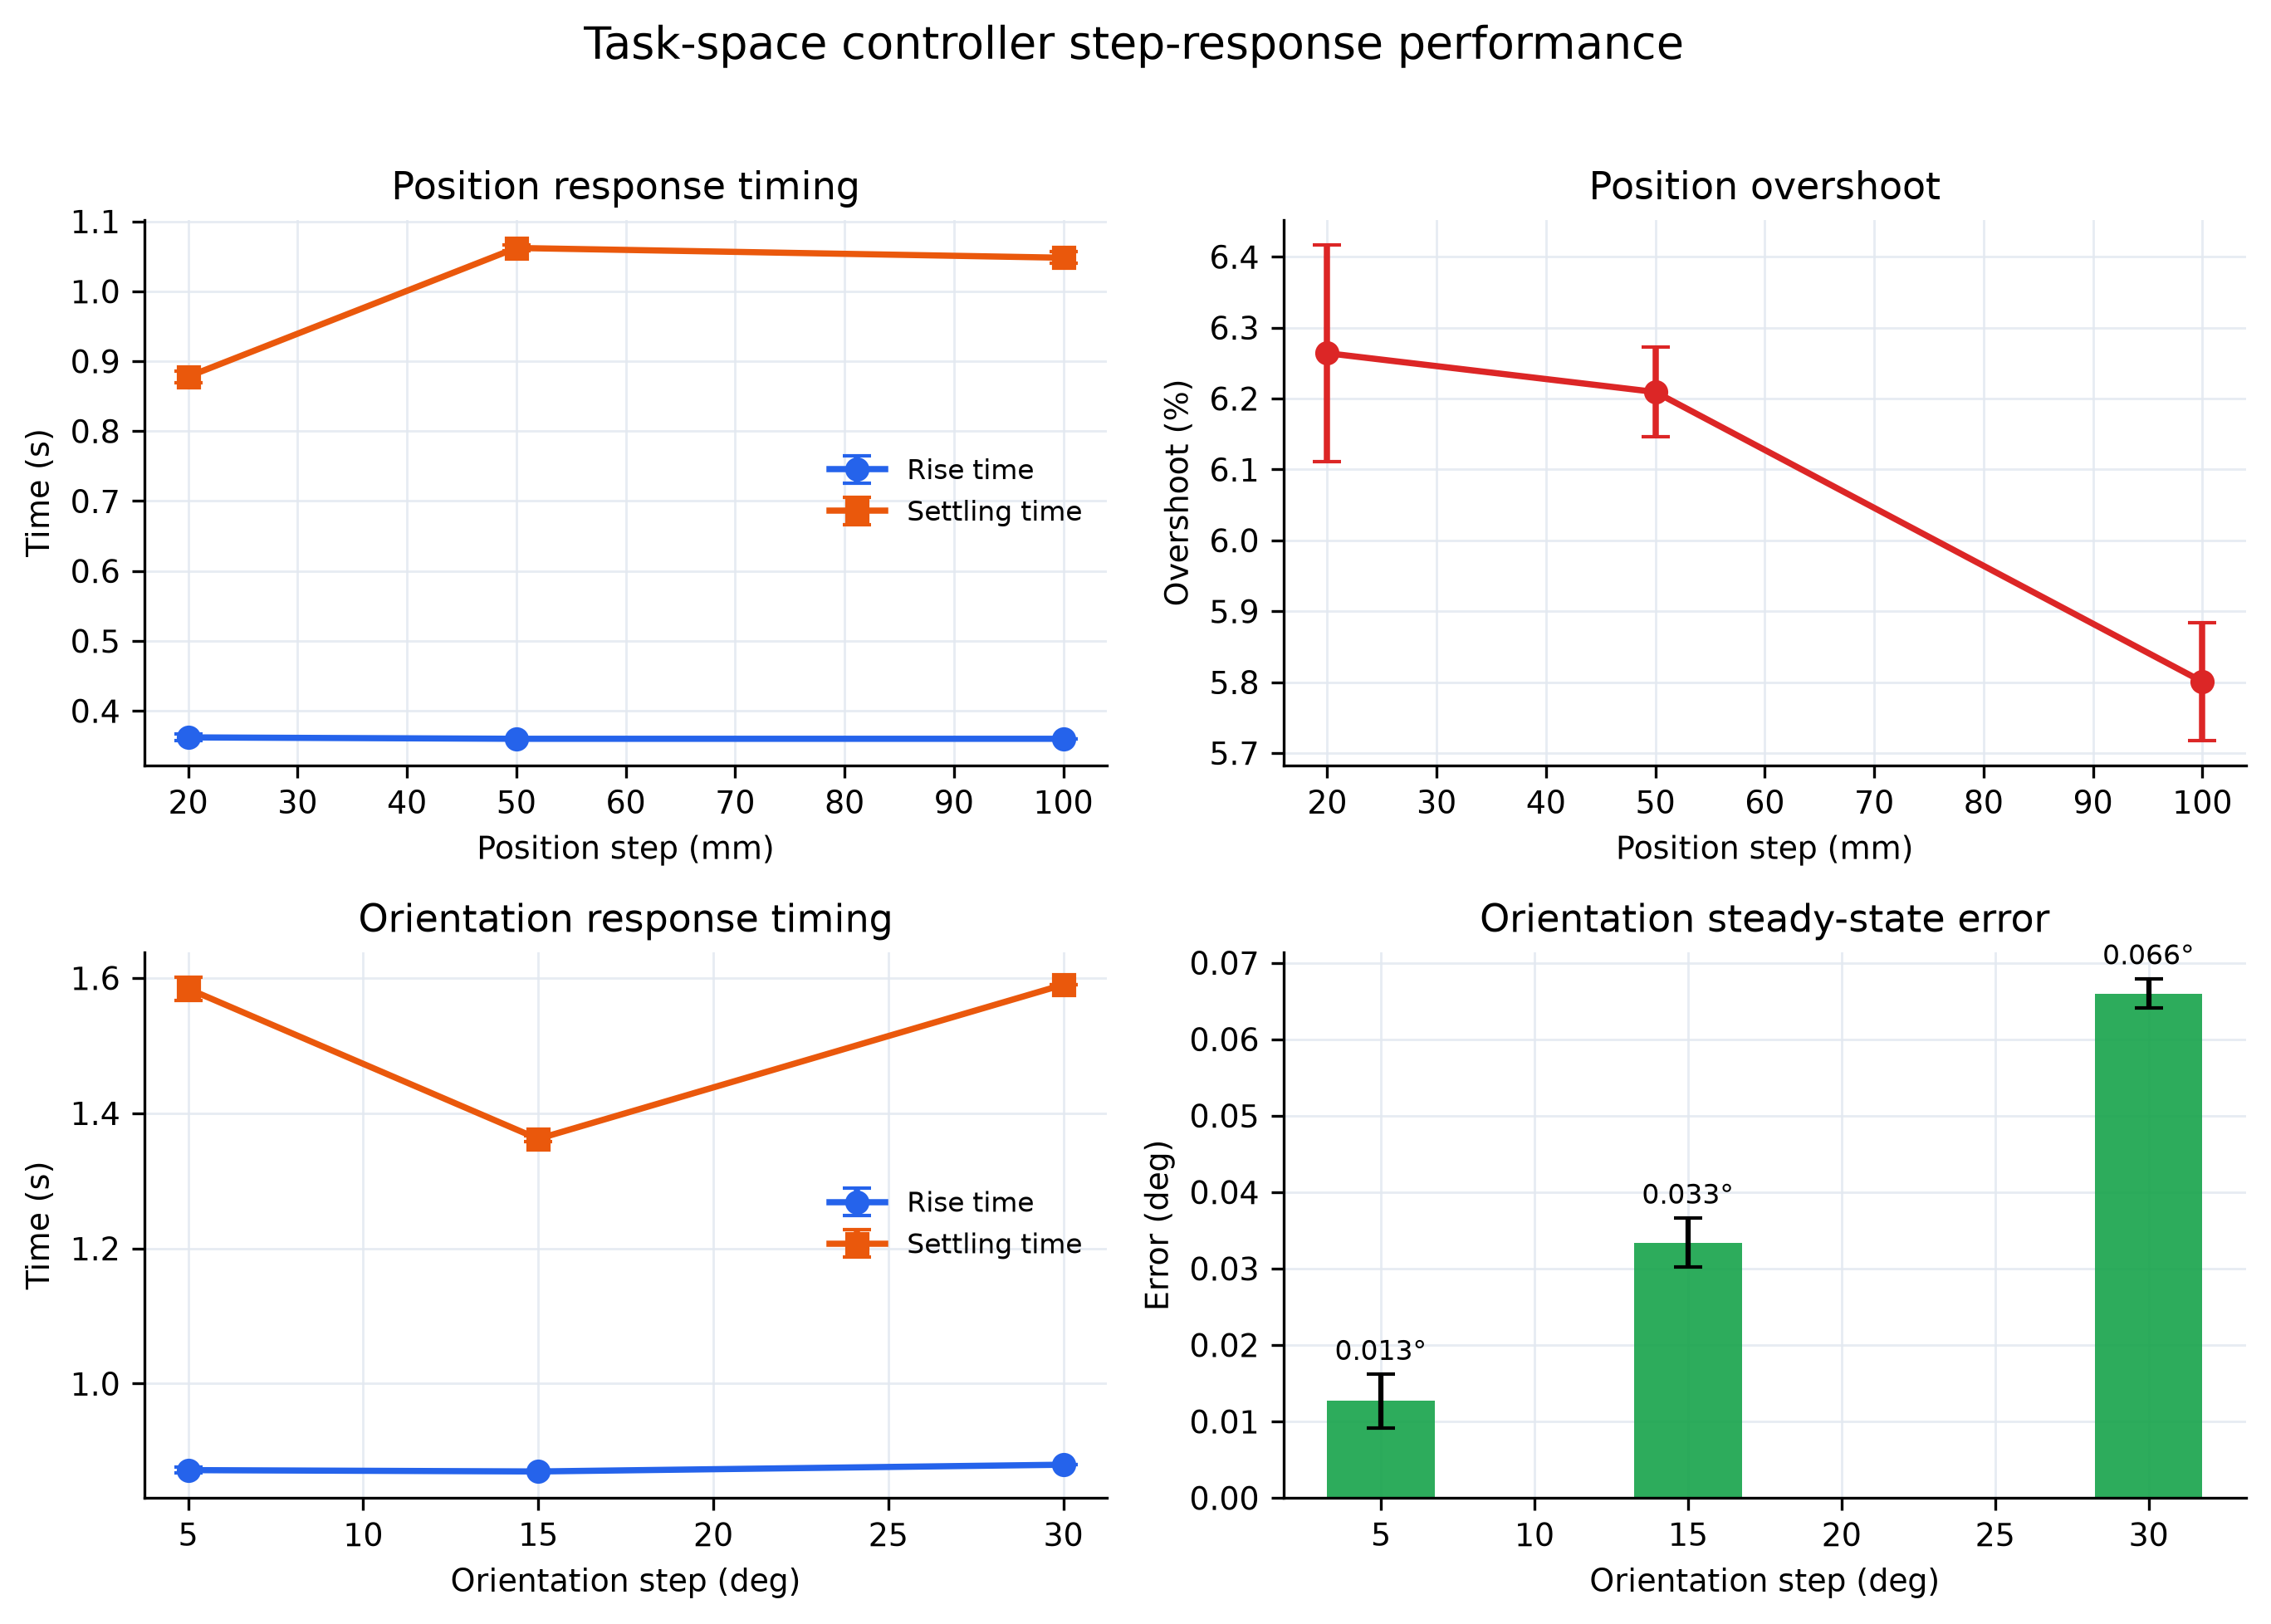
\includegraphics[width=.94\linewidth]{step_response_summary.png}
\caption{Step-response metrics over the tested translation and rotation magnitudes.}
\label{fig:step-response}
\end{figure}

\subsection{Speed sweep}
The ellipse and figure-eight were each tested at 4, 3, 2 and 1.5 s traversal times with three seeded centre offsets per condition. A run was acceptable if peak position error was at most 50 mm, torque clipping occurred in at most 1\% of samples, and the peak joint-speed ratio was at most 1. The ratio is the largest measured absolute joint speed divided by its reference speed limit. Compressing the same path in time raises both velocity and acceleration demand.
\begin{table}[!htbp]
\centering\small
\caption{Speed sweep ($n=3$ per condition). Torque clipping was zero in every run.}
\begin{tabular}{lrrrrr}
\toprule
Path & Time (s) & RMSE (mm) & Peak (mm) & Peak speed (\% limit) & Pass\\
\midrule
Ellipse & 4.0 & $18.00\pm0.05$ & $25.97\pm0.26$ & $19.92\pm0.07$ & 3/3\\
Ellipse & 3.0 & $27.36\pm0.11$ & $37.89\pm0.36$ & $27.34\pm0.10$ & 3/3\\
Ellipse & 2.0 & $48.55\pm0.21$ & $66.83\pm0.18$ & $42.44\pm0.29$ & 0/3\\
Ellipse & 1.5 & $68.46\pm0.11$ & $94.07\pm0.14$ & $55.21\pm0.12$ & 0/3\\
Figure-eight & 4.0 & $24.78\pm0.17$ & $40.22\pm0.47$ & $20.54\pm0.10$ & 3/3\\
Figure-eight & 3.0 & $36.70\pm0.09$ & $58.06\pm0.29$ & $27.81\pm0.20$ & 0/3\\
Figure-eight & 2.0 & $54.18\pm0.13$ & $87.53\pm0.54$ & $35.58\pm0.22$ & 0/3\\
Figure-eight & 1.5 & $61.92\pm0.01$ & $102.52\pm0.07$ & $38.69\pm0.31$ & 0/3\\
\bottomrule
\end{tabular}
\end{table}

The figure-eight first failed at 3 s and the ellipse at 2 s. As traversal time fell, peak tracking error increased. The highest mean peak joint-speed utilization was 55.21\%, and no run clipped torque. The 50 mm tracking-error threshold was therefore crossed before the monitored limits.

\begin{figure}[H]
\centering
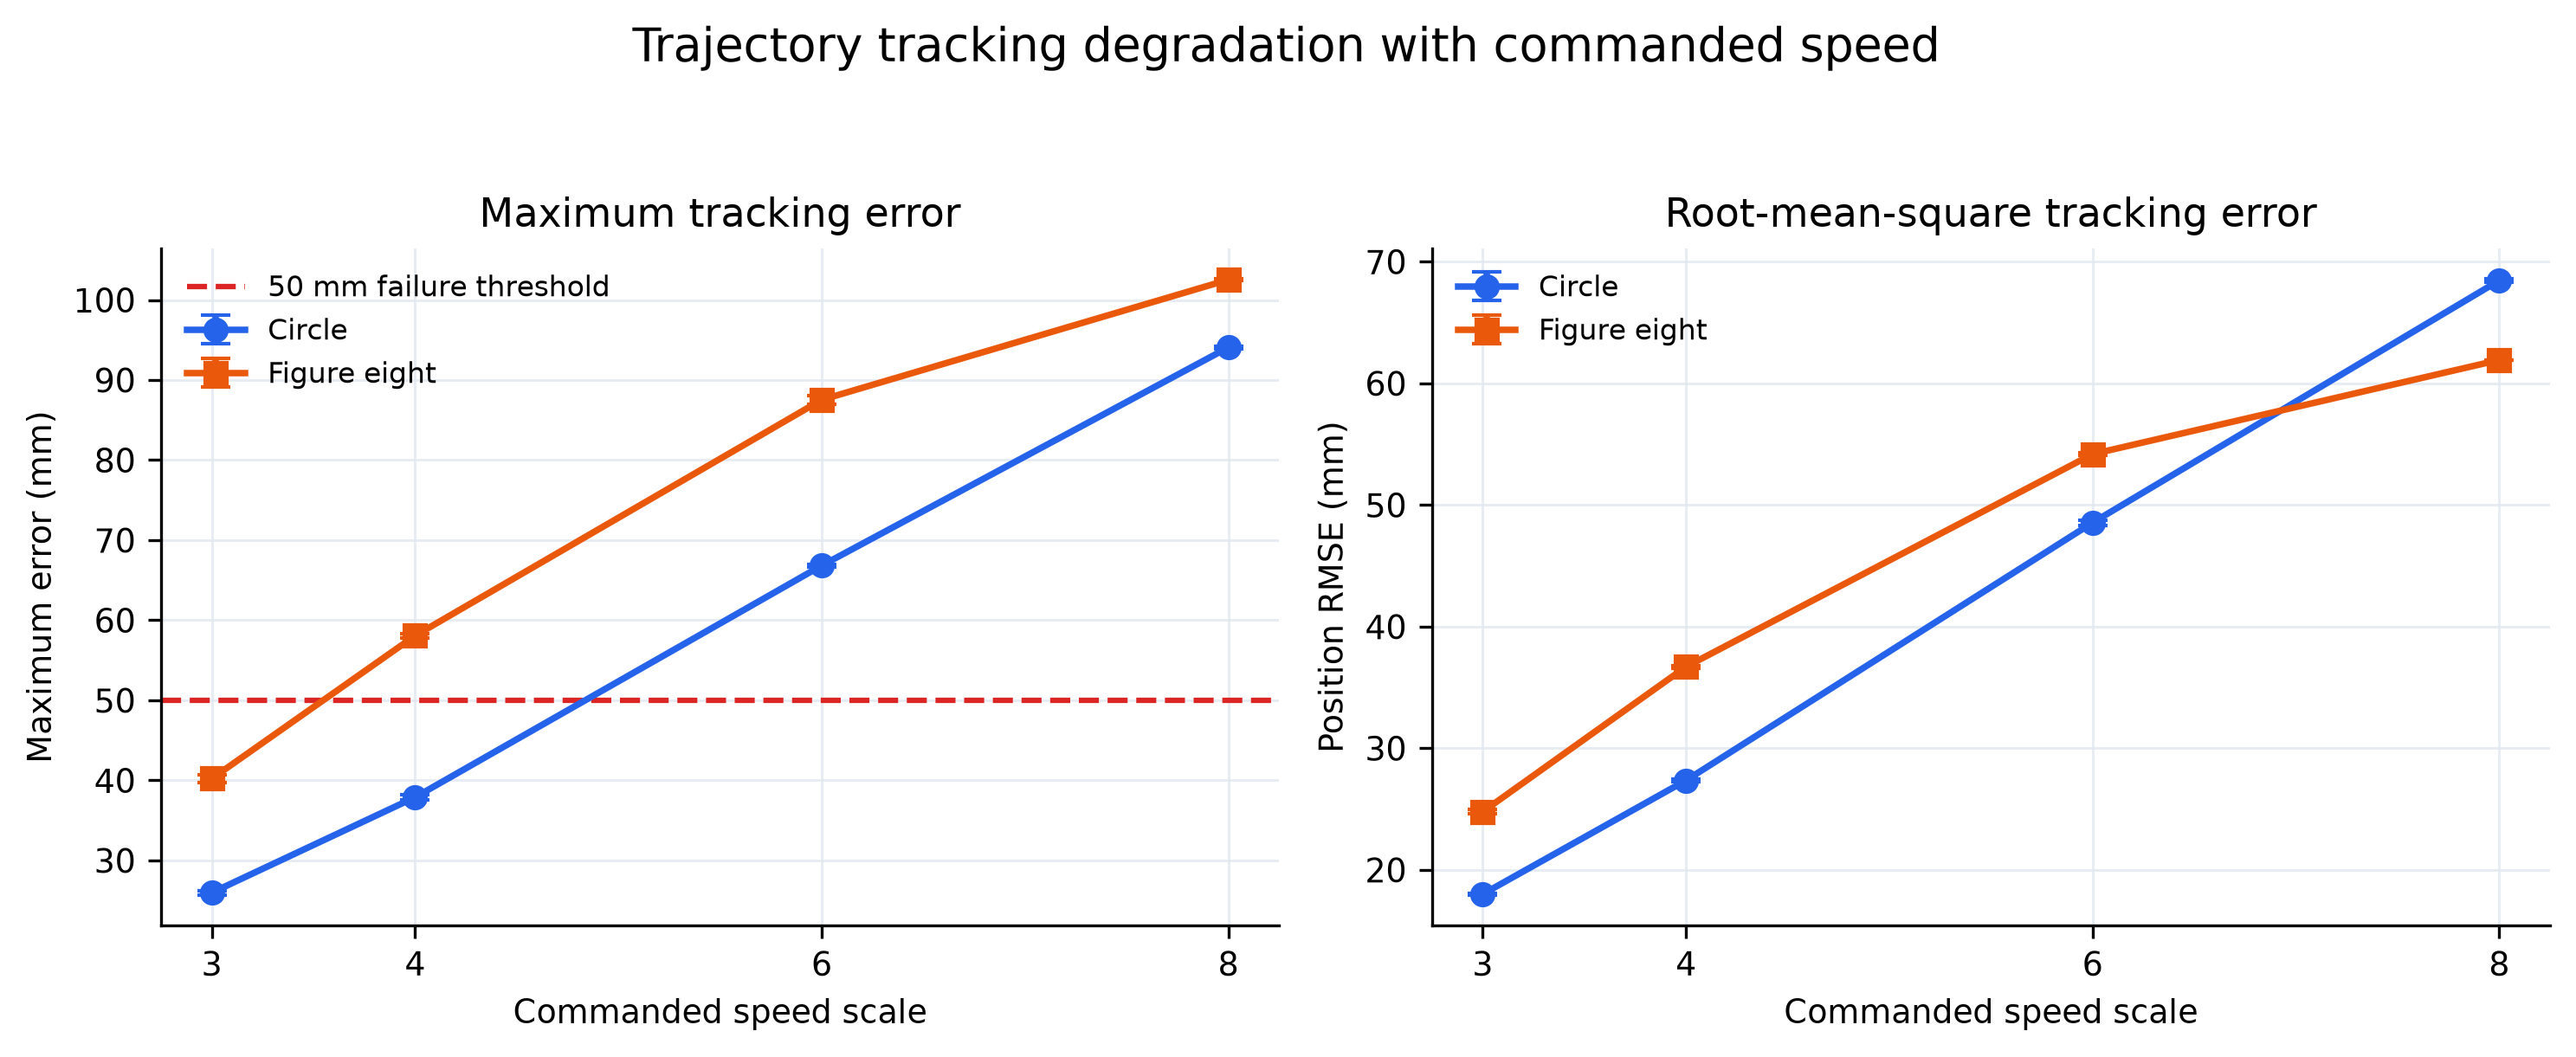
\includegraphics[width=.94\linewidth]{speed_limit_tracking.png}
\caption{Peak and RMS tracking errors as commanded speed increases. The peak-error criterion is 50 mm.}
\label{fig:speed-tracking}
\end{figure}

At 4 s, all six speed-sweep trials passed. At 3 s, all three ellipse trials passed and all three figure-eight trials failed. The figure-eight's $y$ reference contains a second harmonic, which increases acceleration demand at a given phase rate. For either path, acceleration demand increases with the square of the speed-up.

The logged summaries capture peak joint speed, torque clipping and tracking error. Joint acceleration was outside the measured criteria. Classifying transients as gradual, oscillatory or unstable would require time-series analysis.

\subsection{Static load and disturbance rejection}
The controller held a fixed pose for 6 s with five seeded trials per condition. A constant downward hand force of $mg$ represented an unmodeled static load. This test represents weight without added inertia. Separate trials applied a 0.25 s lateral force pulse beginning at 2 s. Recovery is the time from the end of the pulse window to the first 0.2 s interval continuously within 10 mm of the reference. Residual error is averaged over the last 0.5 s. The standard deviation of error in the final window measures residual variation. The experiment did not estimate temporal drift or resolve vibration frequency.
\begin{table}[!htbp]
\centering\small
\caption{Hold tests ($n=5$ per condition). A dash indicates that the recovery criterion was never met.}
\begin{tabular}{lrrr}
\toprule
Condition & Peak (mm) & Recovery (s) & Residual (mm)\\
\midrule
Nominal hold & $2.53\pm0.21$ & $0.000\pm0.000$ & $1.84\pm0.28$\\
0.5 kg equivalent & $25.53\pm0.07$ & --- & $24.73\pm0.16$\\
1 kg equivalent & $51.99\pm0.04$ & --- & $50.74\pm0.14$\\
2 kg equivalent & $106.55\pm0.02$ & --- & $103.46\pm0.06$\\
10 N pulse & $40.73\pm0.04$ & $0.450\pm0.000$ & $2.04\pm0.14$\\
20 N pulse & $81.28\pm0.06$ & $0.520\pm0.000$ & $2.24\pm0.29$\\
40 N pulse & $161.60\pm0.12$ & $0.898\pm0.004$ & $2.22\pm0.48$\\
\bottomrule
\end{tabular}
\end{table}

Residual error increased from 1.84 mm nominally to 103.46 mm under the 2 kg equivalent load (Figure~\ref{fig:payload}). This is consistent with a PD controller balancing a persistent unmodeled force through position error.

\begin{figure}[!htbp]
\centering
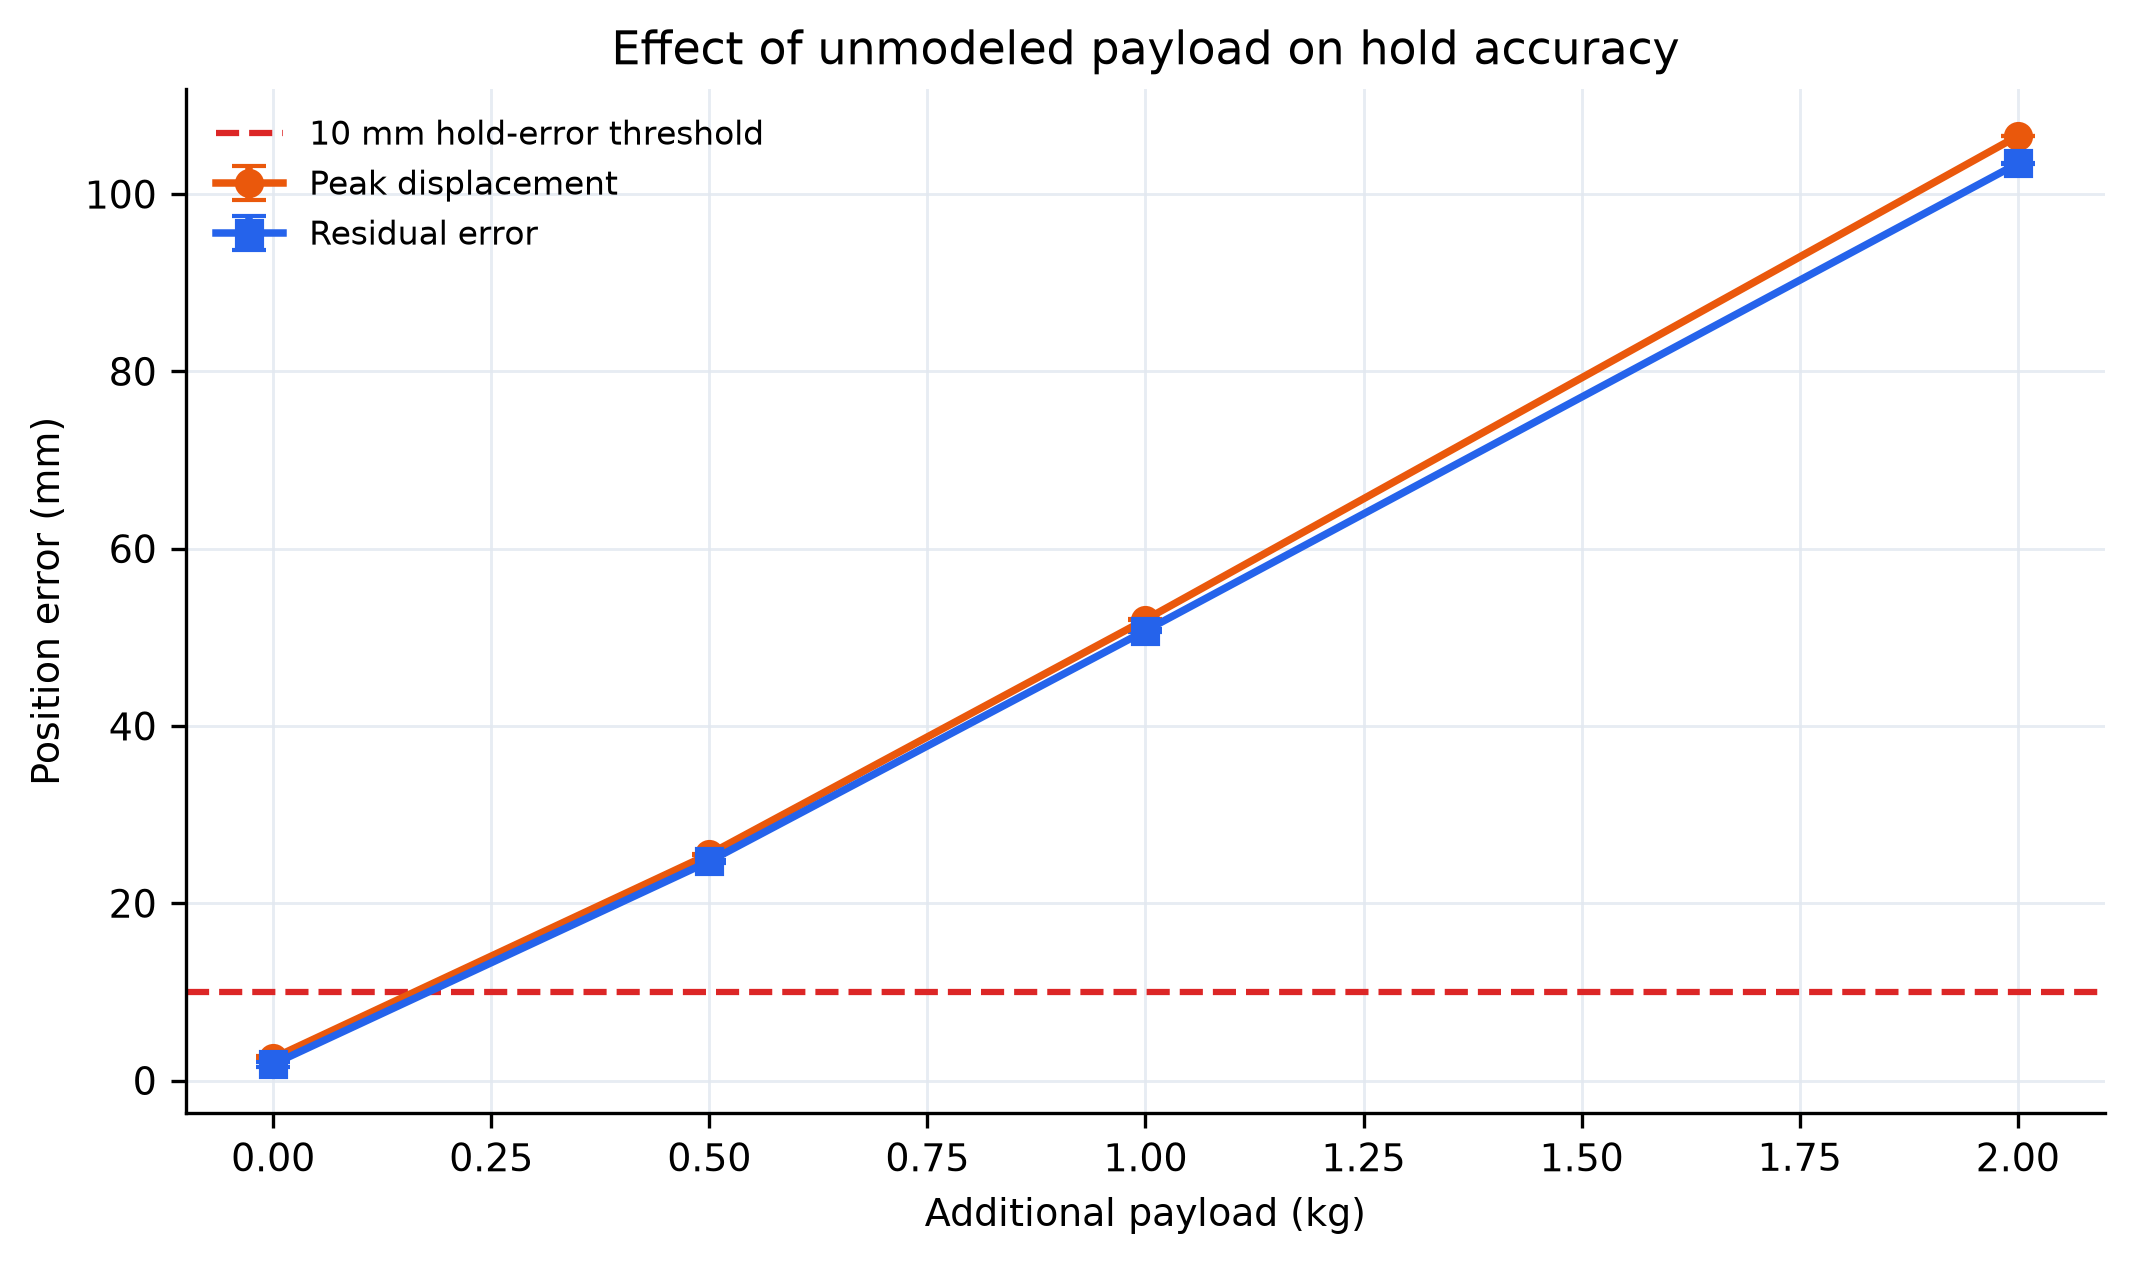
\includegraphics[width=.85\linewidth]{robustness_payload.png}
\caption{Peak and residual position errors under sustained downward force.}
\label{fig:payload}
\end{figure}

\noindent\begin{minipage}{\linewidth}
\begingroup
\centering
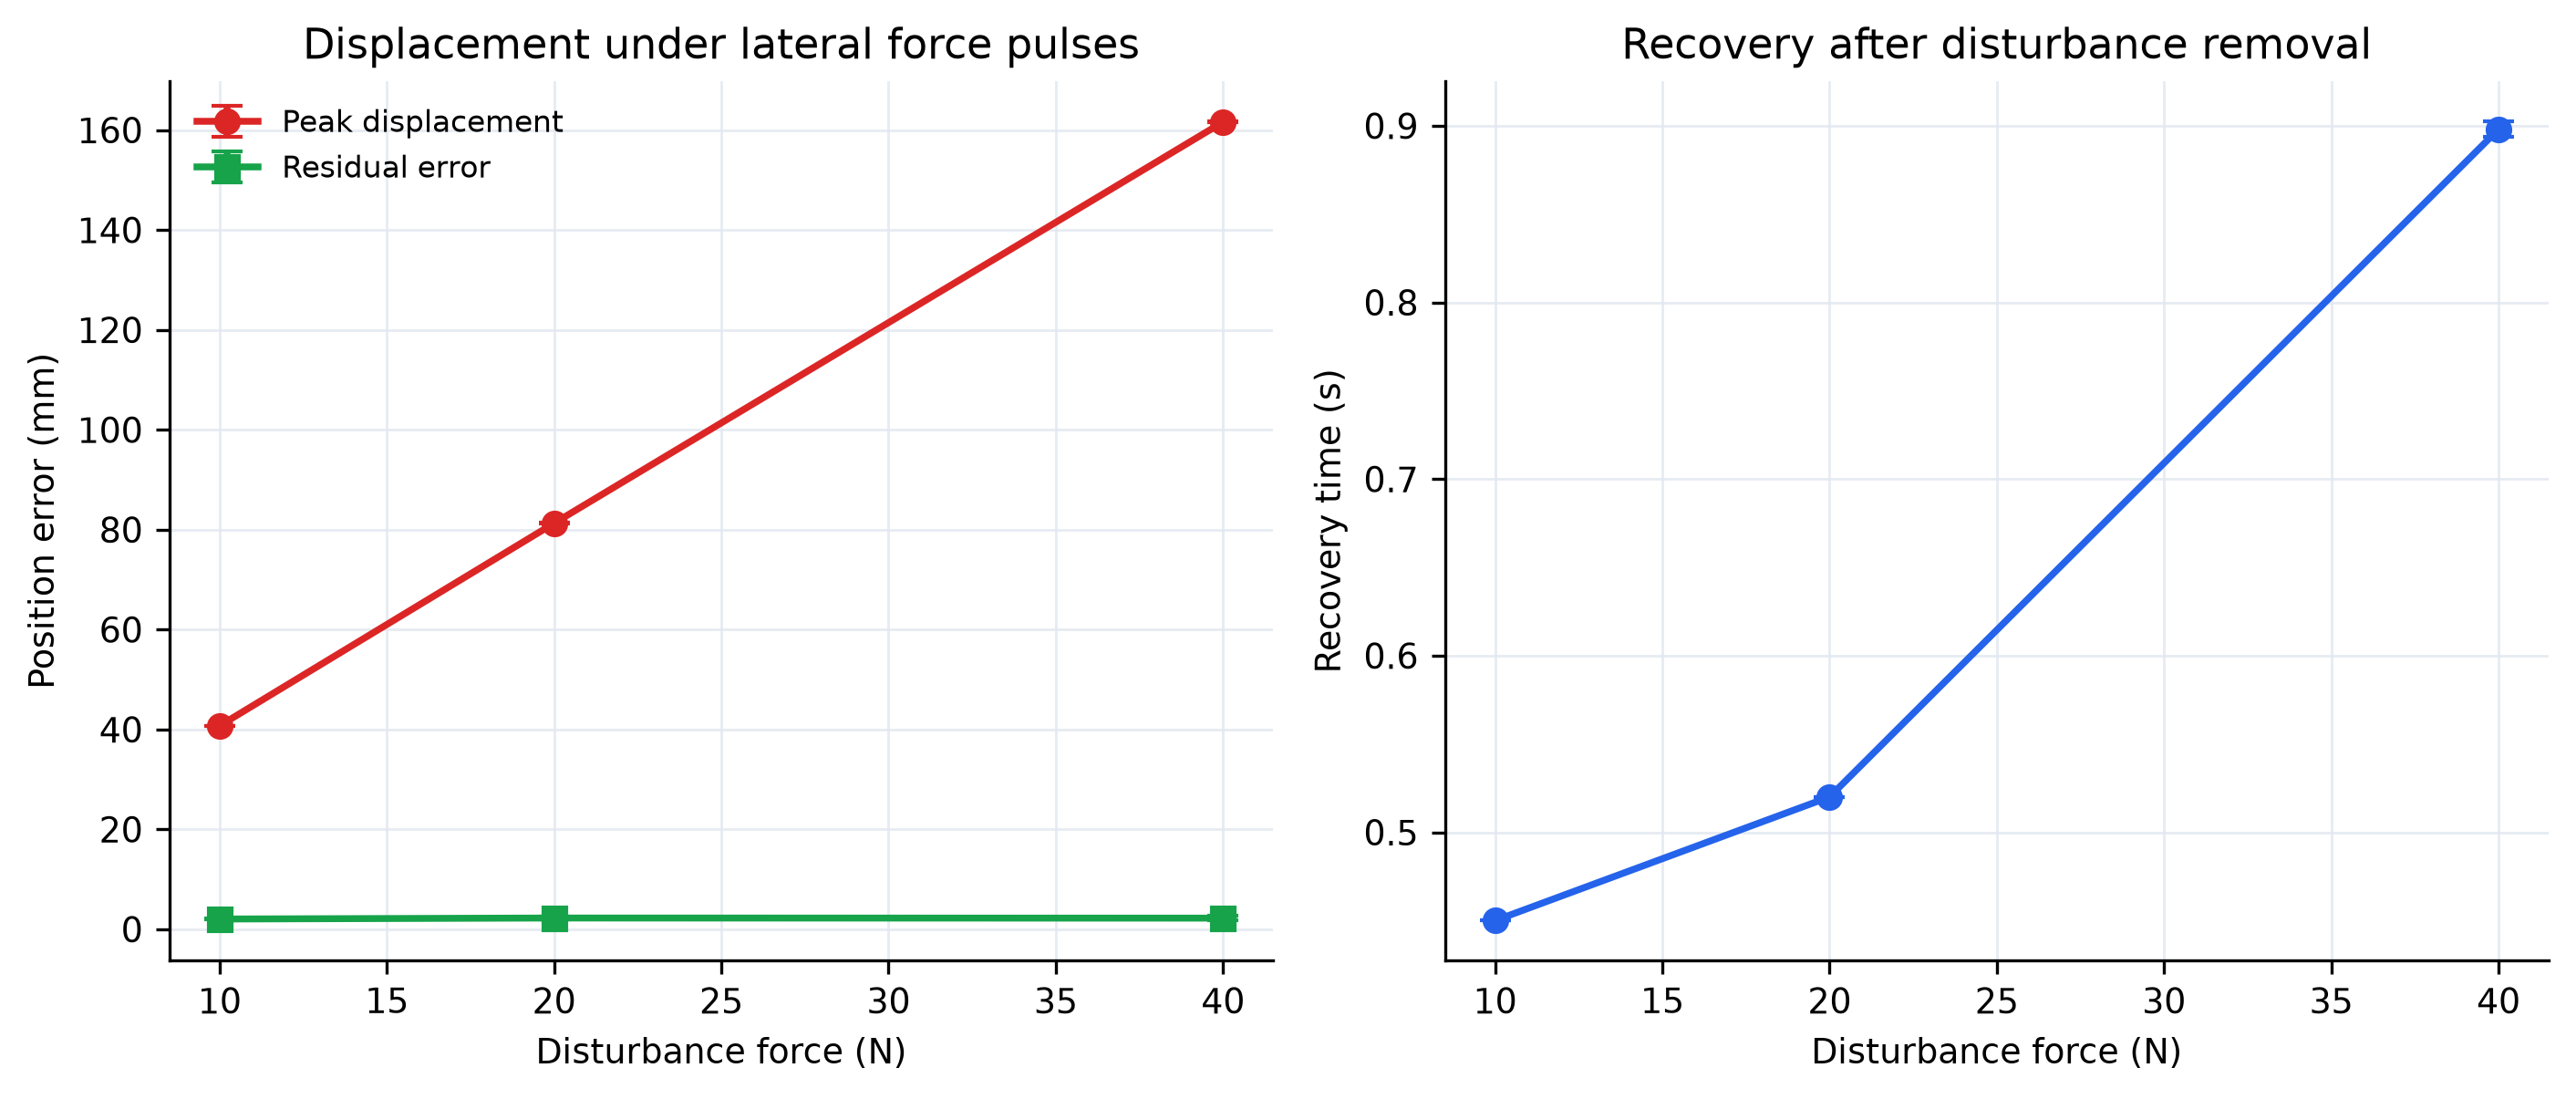
\includegraphics[width=.85\linewidth]{robustness_disturbance.png}
\captionof{figure}{Peak displacement and recovery after brief lateral force pulses.}
\label{fig:disturbance}
\endgroup
\vspace{.65em}

The 40 N pulse produced a mean peak displacement of 161.60 mm and a mean recovery time of 0.898 s (Figure~\ref{fig:disturbance}). Across the hold tests, mean error variation in the final measurement window remained below 0.003 mm and sampled torque clipping was zero. The tested positions and loads did not isolate Jacobian conditioning or motion at the workspace boundary.
\end{minipage}

\section{Grasp and Randomized Five-Block Stacking}
\subsection{Standalone grasp-and-lift}
The standalone scripted trial approaches the cube, closes the gripper and raises the hand. Success requires at least 50 mm of net cube lift. The archived run increased cube height by 106.97 mm from the first logged sample to the end, with 8.28 mm hand position RMSE and 0 clipped samples. This single trial illustrates the manipulation sequence.

The grasp reference is 90 mm above the cube centre at the hand body, and the subsequent lift target adds 120 mm. This standalone experiment uses cubic smoothstep motion timing, with zero commanded endpoint velocity. Its height trace shows when the cube starts moving with the hand and whether the new height persists through the final hold.

\begin{figure}[!htbp]
\centering
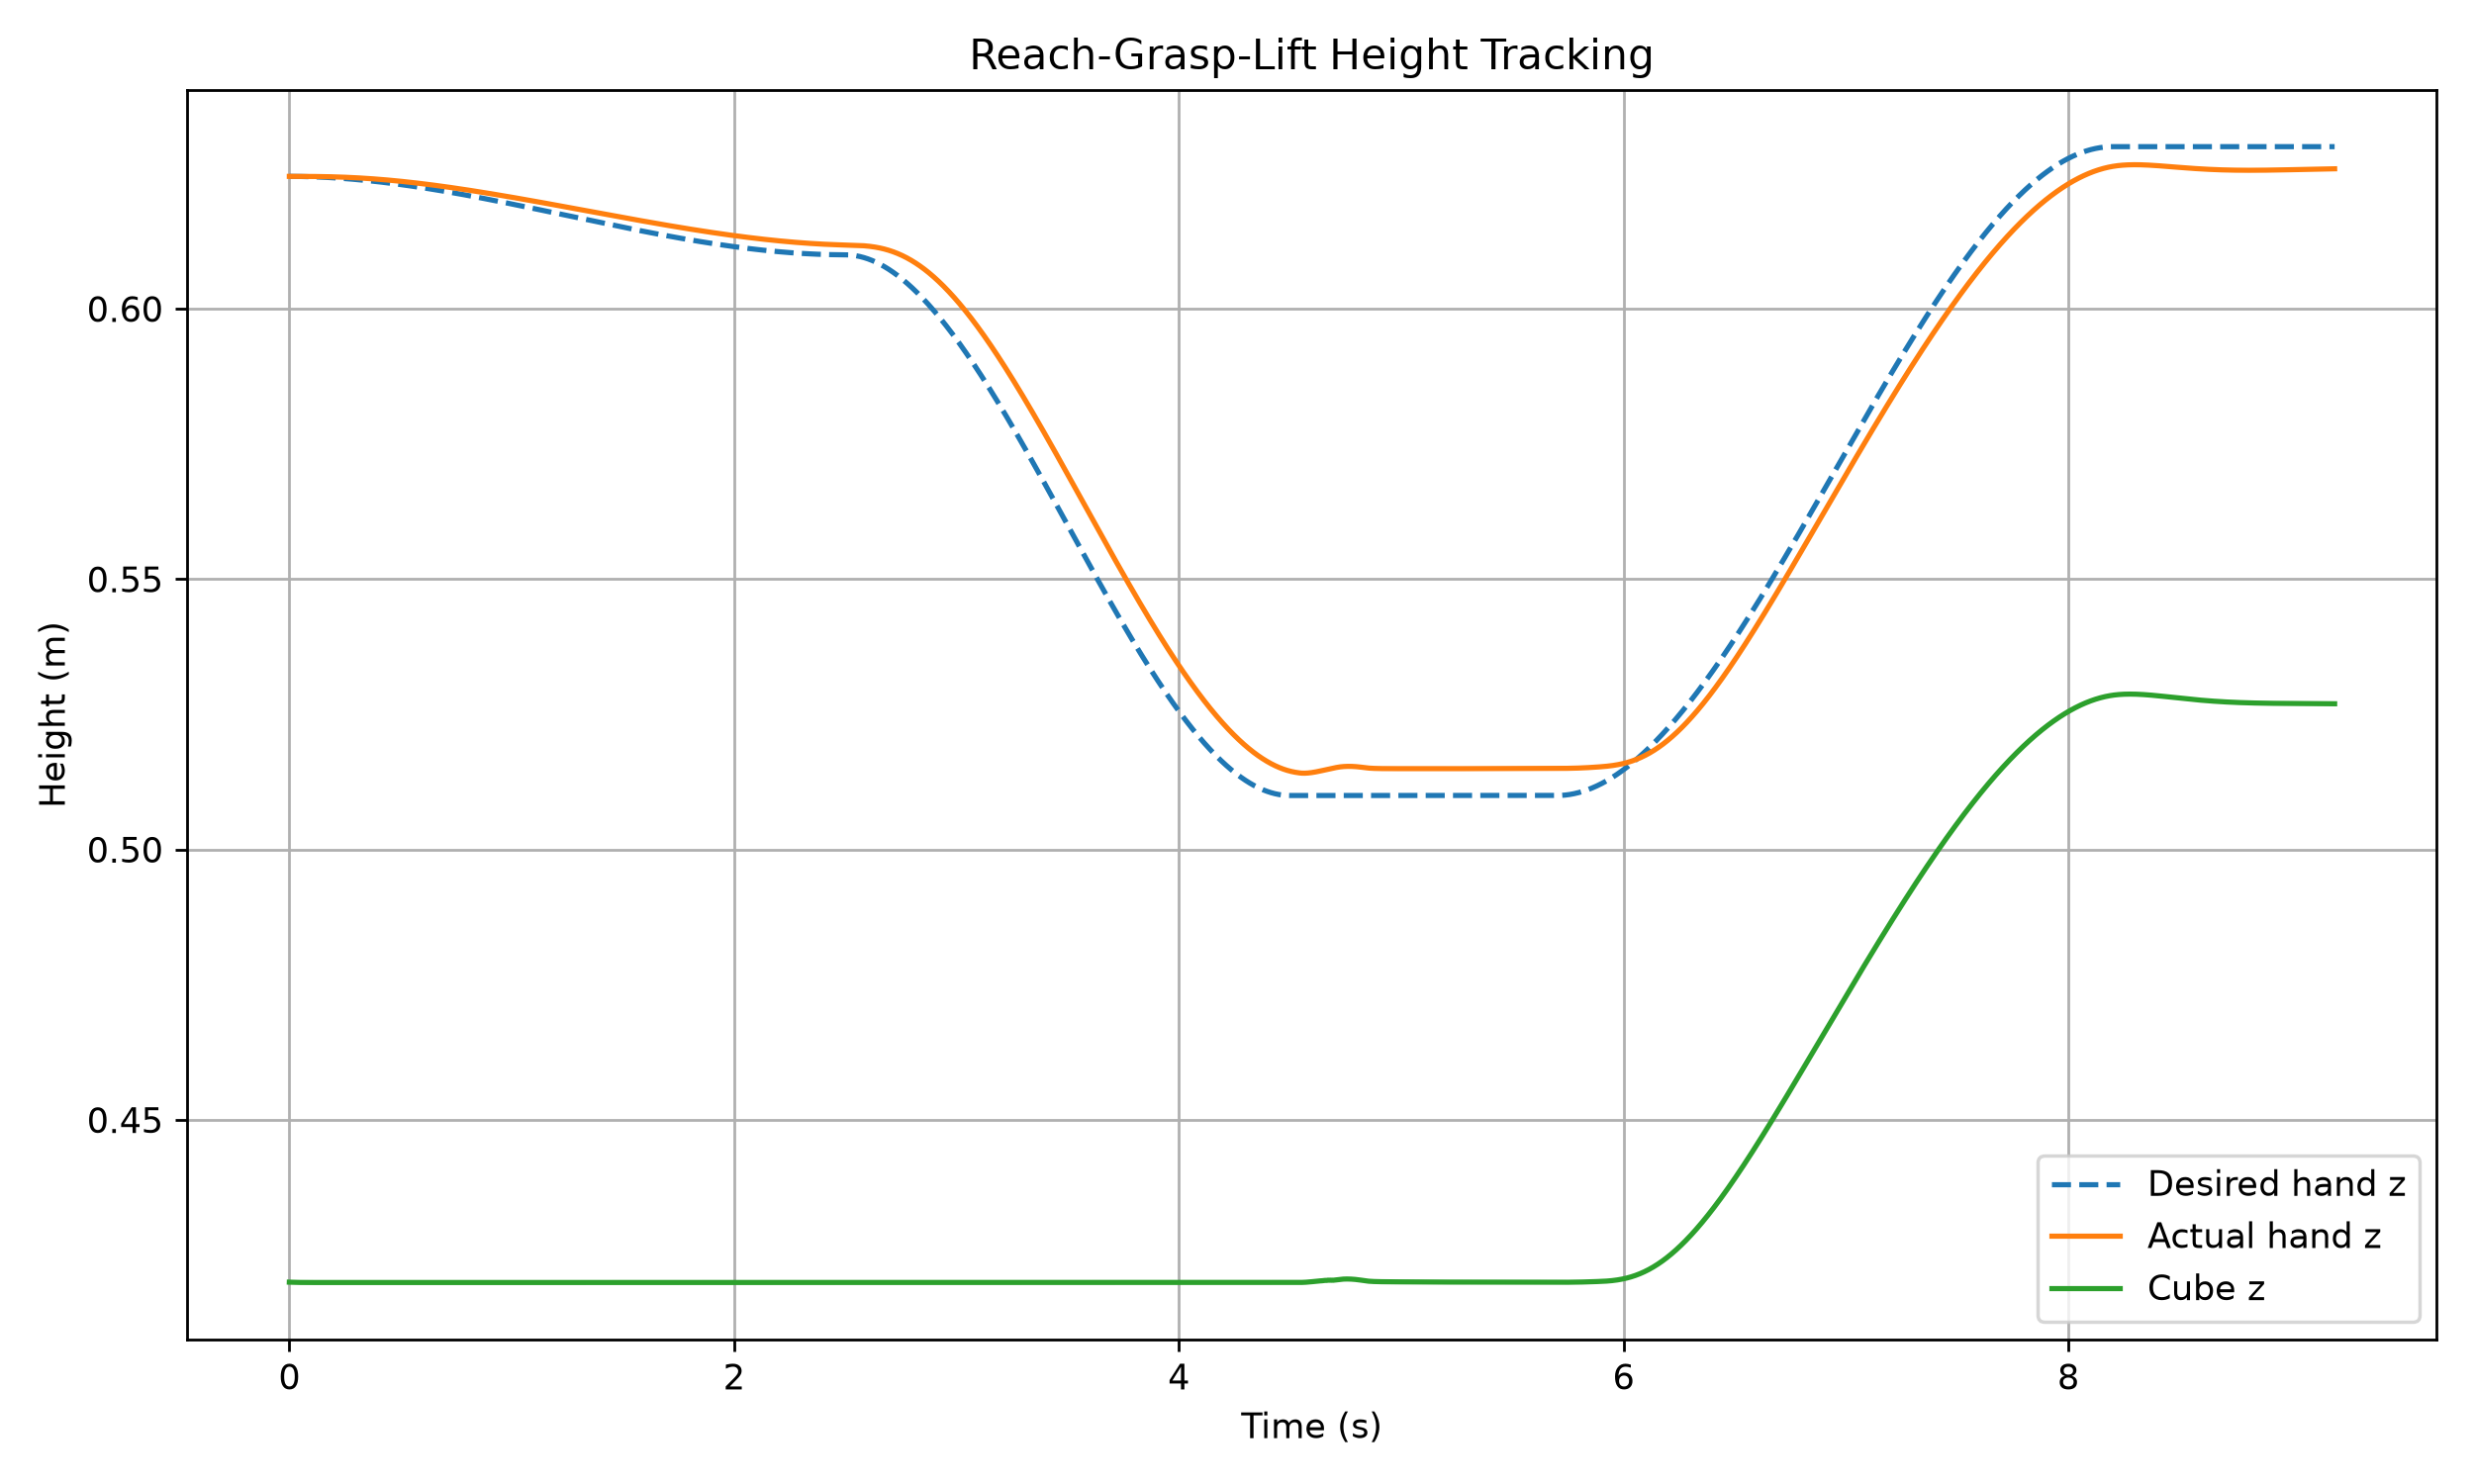
\includegraphics[width=.83\linewidth]{height_tracking.png}
\caption{Measured hand and cube height during the approach, grasp, lift and hold.}
\label{fig:grasp-lift}
\end{figure}

The 4,600 recorded samples cover the 2.5 s approach, 2.0 s descent, 1.2 s gripper closure, 2.5 s lift and 1.0 s hold. Cube height increased from 0.42000 m to 0.52697 m through simulated contact with the fingers. The maximum hand position error was 16.29 mm and the maximum orientation error was $0.990^\circ$. The final hand position error was 4.20 mm.

\subsection{Randomized two-tower task}
For each of ten seeded episodes, five labelled cubes (A--E) start at $z=0.42$ m. Pickup coordinates range from 0.470 to 0.565 m in $x$ and from $-0.13$ to 0.13 m in $y$. Rejection sampling keeps block centres at least 60 mm apart and each pickup corridor at least 140 mm from both tower centres. A random permutation assigns three labels to tower 1 and two to tower 2, in bottom-to-top order. The towers are centred at $(0.64,-0.04)$ and $(0.64,0.12)$ m. Target heights are 0.42, 0.46 and 0.50 m as applicable. Each episode log records its seed, layout, requested order, completion time and placement errors.

Quintic interpolation connects task-derived hand poses for approach, descent, lift, transit, placement and retreat. Standard motion phases last 2.5 s, gripper holds 1 s, safe-transit moves 1.5 s and settling 0.5 s. The controller reads exact block positions, checks grasp geometry after lifting and can retry a grasp once. It selects which tower to build first using the sampled geometry while preserving each requested bottom-to-top order. The placement reference adds a level-specific $x$ compensation of 8, 16 or 25 mm. Scoring uses the nominal block-centre targets.

A successful episode finishes both requested towers in order within 120 s. Every block must finish at most 35 mm from its target in the horizontal plane and within 25 mm vertically. All ten episodes passed (100\%). Successful episodes took $112.63\pm0.00$ s of simulation time, reflecting the fixed phase durations across these runs. Across all 50 block placements, final Euclidean error was $14.87\pm6.51$ mm (mean and sample standard deviation). The ten episode-average errors were $14.87\pm0.70$ mm. The first spread describes variation among individual placements and the second describes variation among episode averages. Episode maxima ranged from 22.27 to 27.55 mm.
\begin{table}[!htbp]
\centering\small
\caption{Euclidean final centre error by level, pooled over placements.}
\begin{tabular}{lrr}
\toprule
Tower level & Placements & Error (mm)\\
\midrule
Level 1 & 20 & $8.29\pm1.89$\\
Level 2 & 20 & $16.47\pm1.73$\\
Level 3 & 10 & $24.84\pm2.05$\\
\bottomrule
\end{tabular}
\end{table}
\begin{figure}[H]
\centering
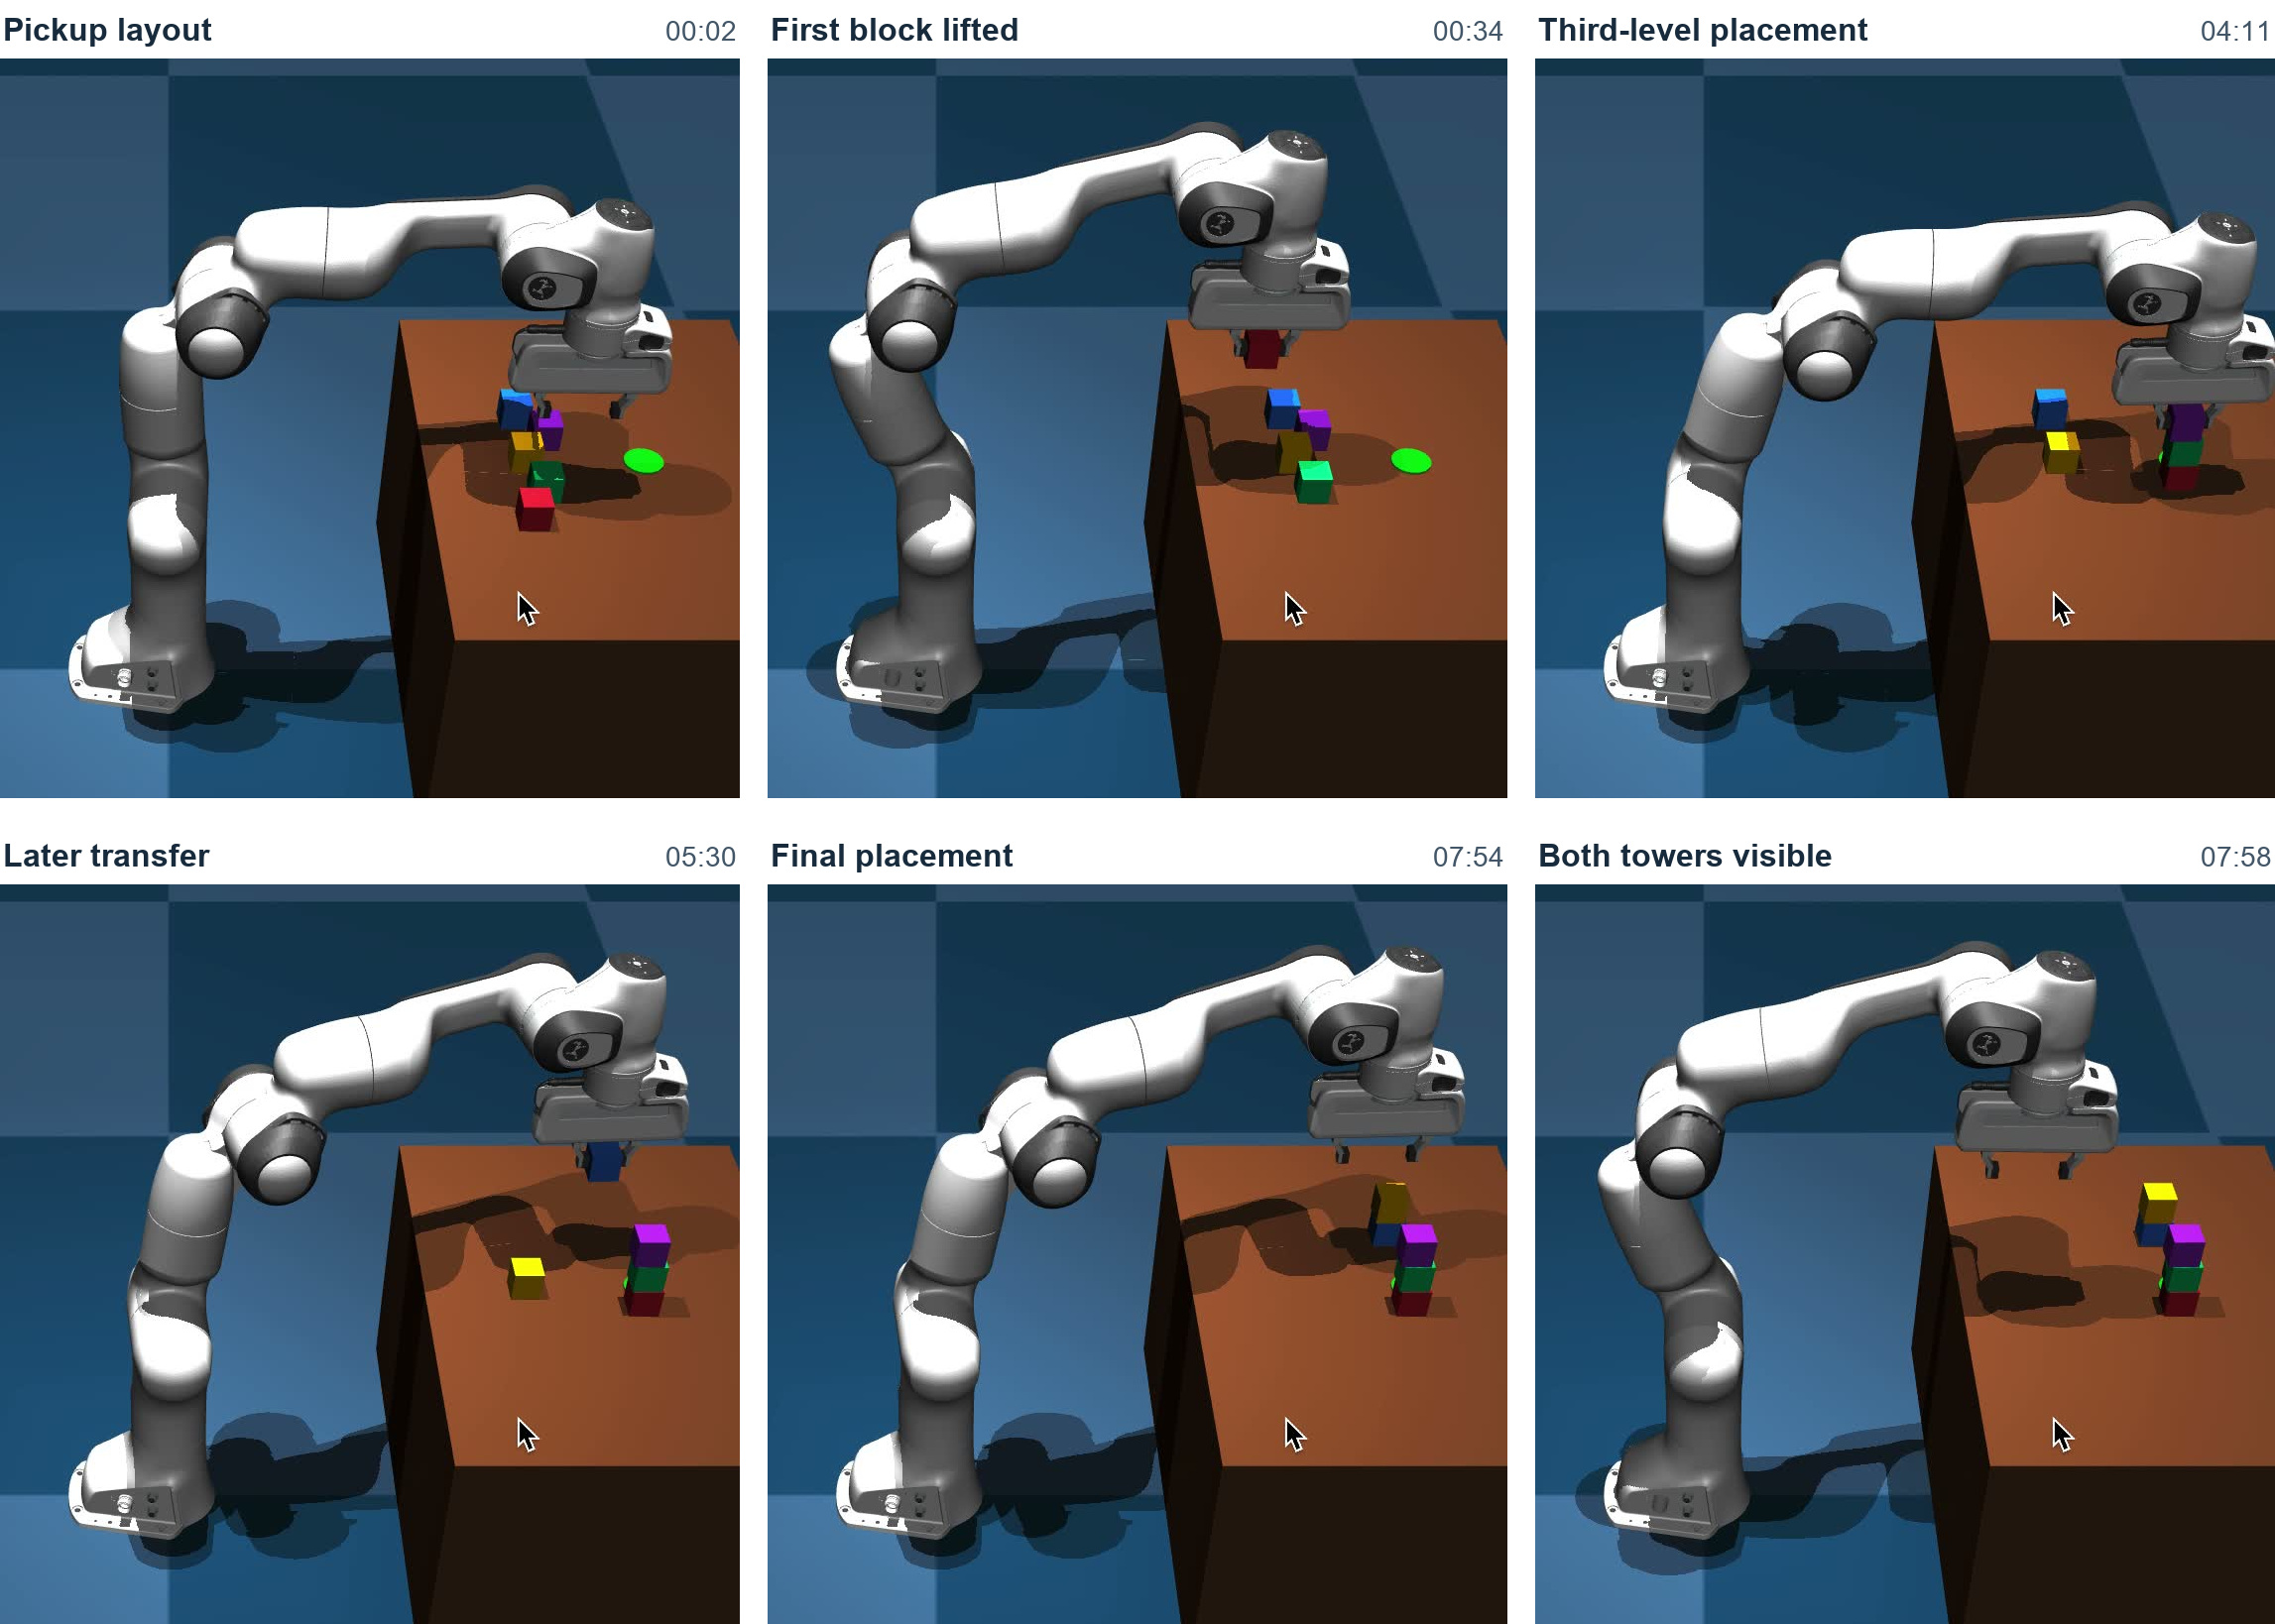
\includegraphics[width=.96\linewidth]{stacking_video_frames.jpg}
\caption{MuJoCo screen-recording frames from stacking episode 1 (seed 2684470948). The requested bottom-to-top orders were A--E--D and B--C. The sequence shows the pickup layout, lift, placement and the two visible towers near the end of the recording. Read left to right, top row first. Timestamps refer to video playback.}
\label{fig:stacking-video}
\end{figure}

\begin{figure}[!htbp]
\centering
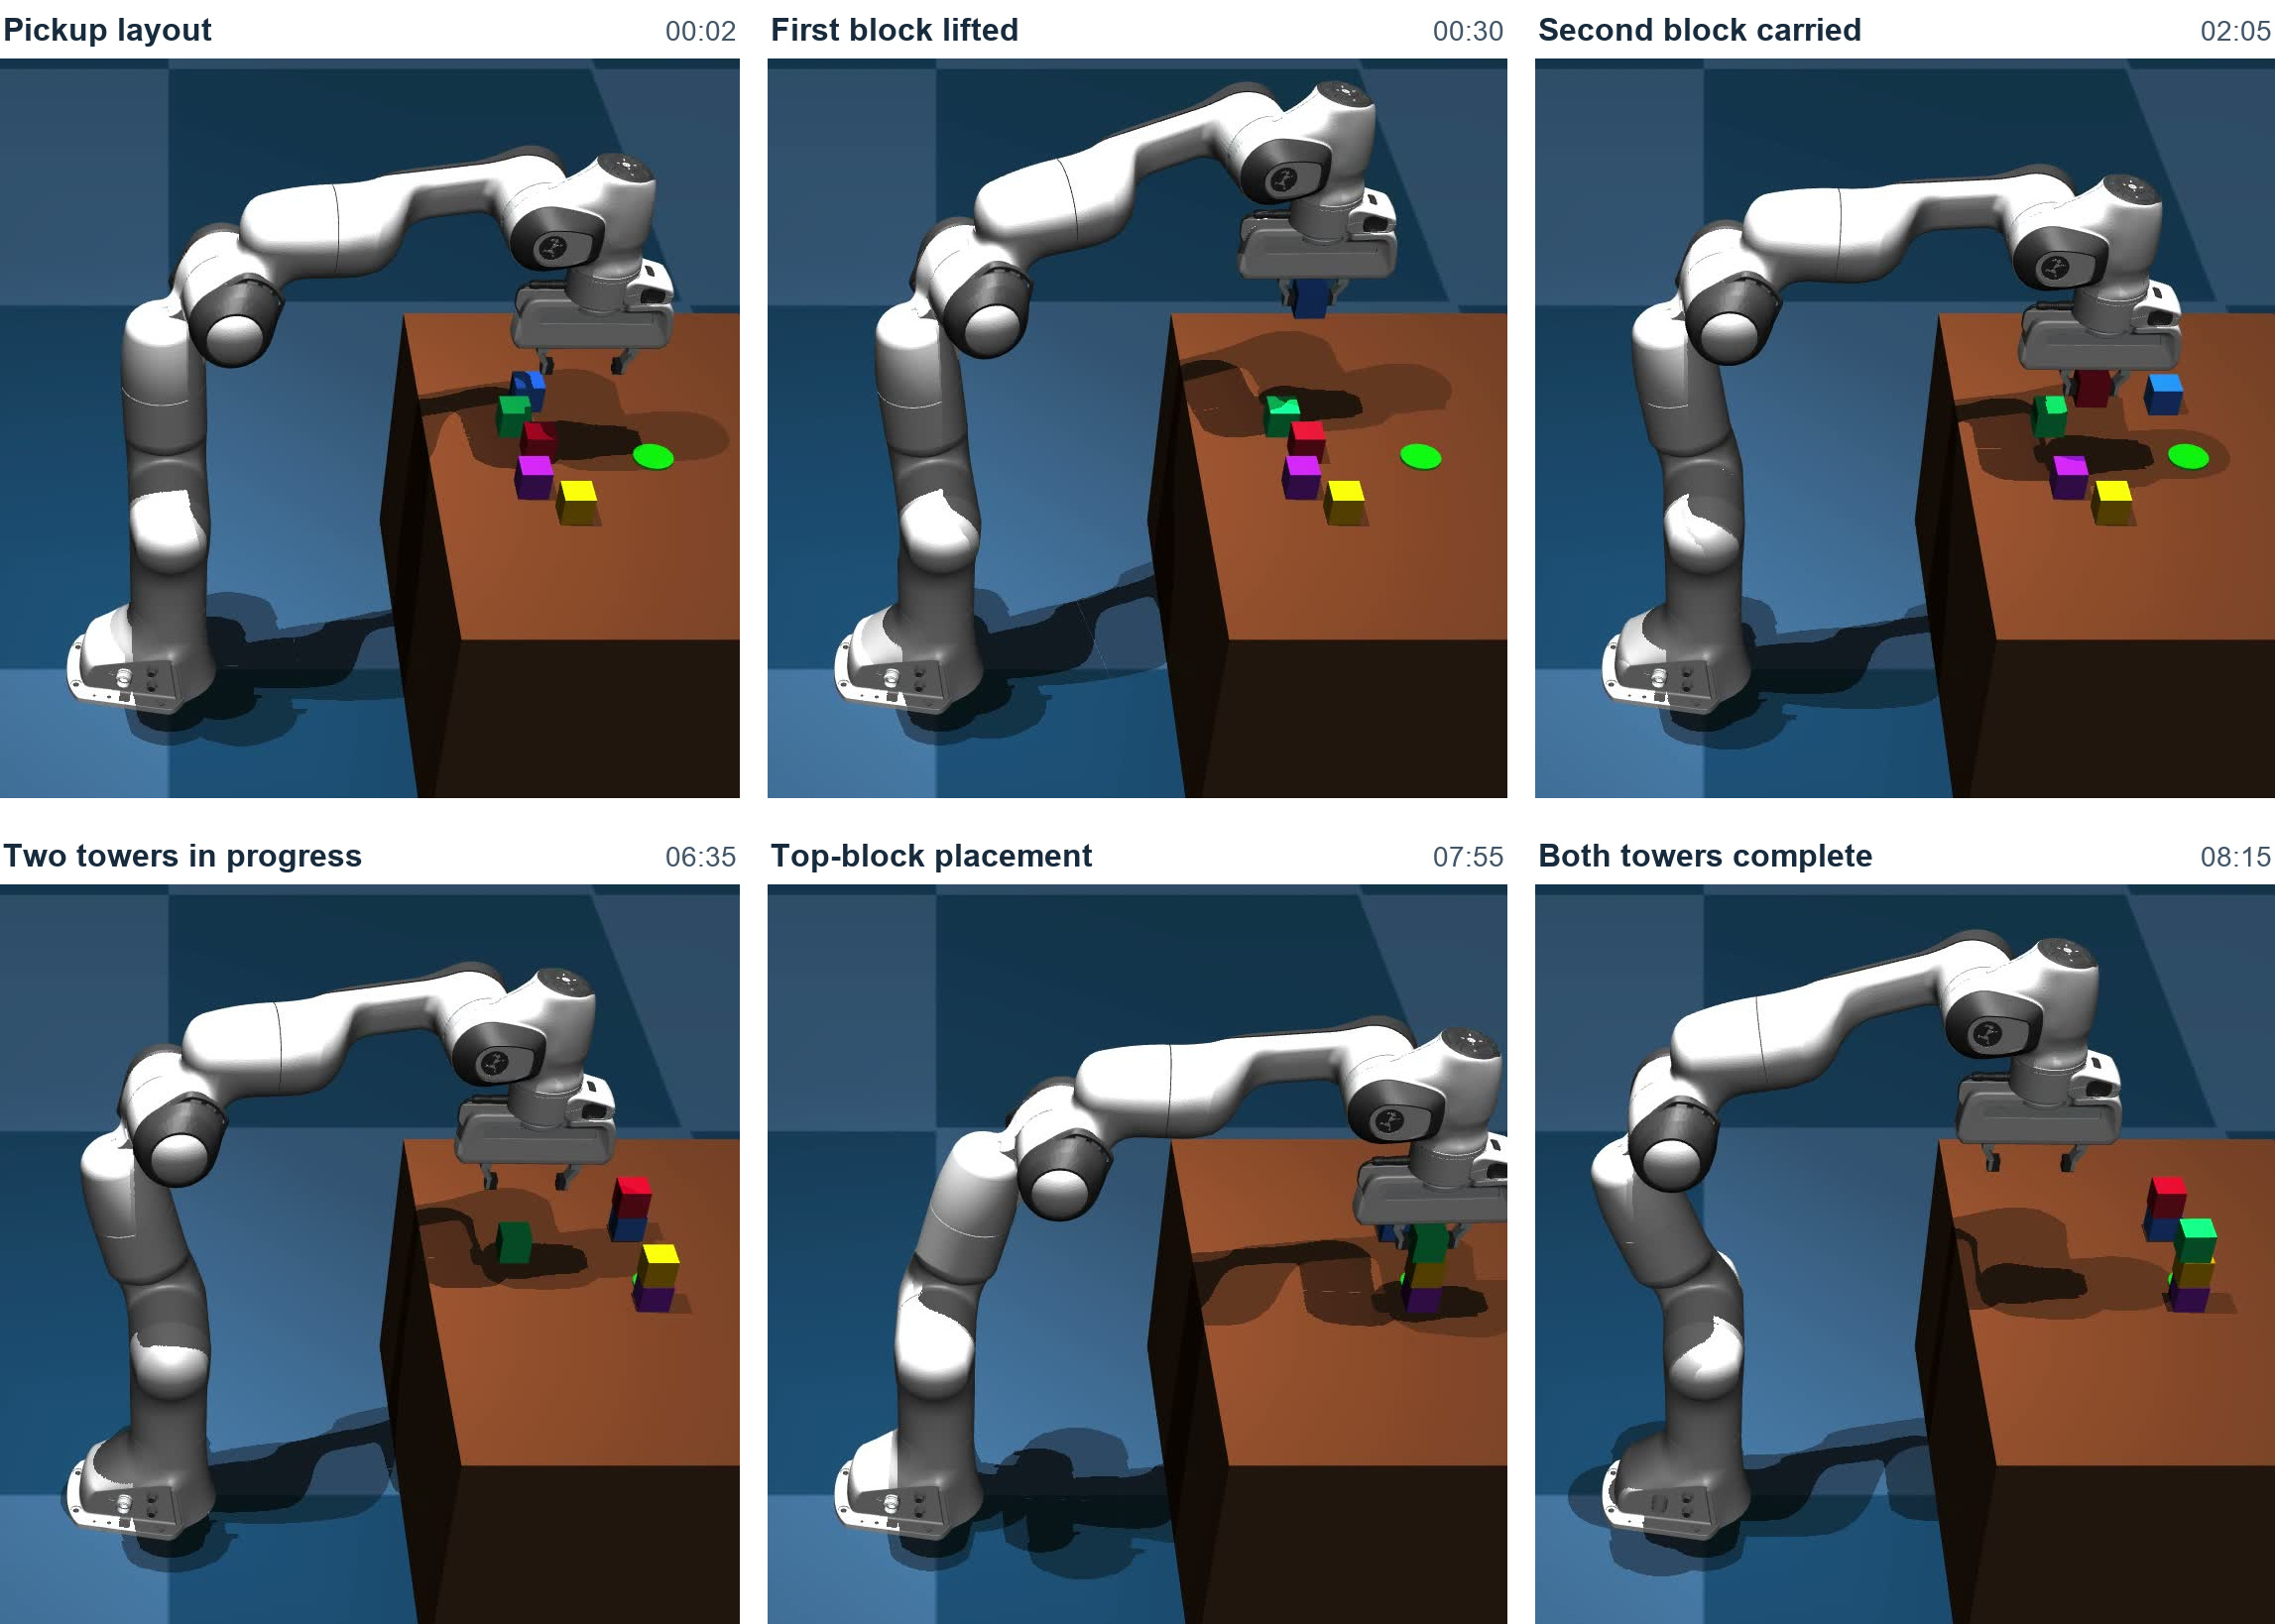
\includegraphics[width=.96\linewidth]{stacking_episode_2_video_frames.jpg}
\caption{Six MuJoCo screen-recording frames from the current-controller replay of stacking episode 2 (seed 4091952314). The requested bottom-to-top orders were D--C--E and B--A. The shorter tower was built first. Read left to right, top row first. Timestamps refer to video playback.}
\label{fig:stacking-episode-two-video}
\end{figure}

\begin{figure}[!htbp]
\centering
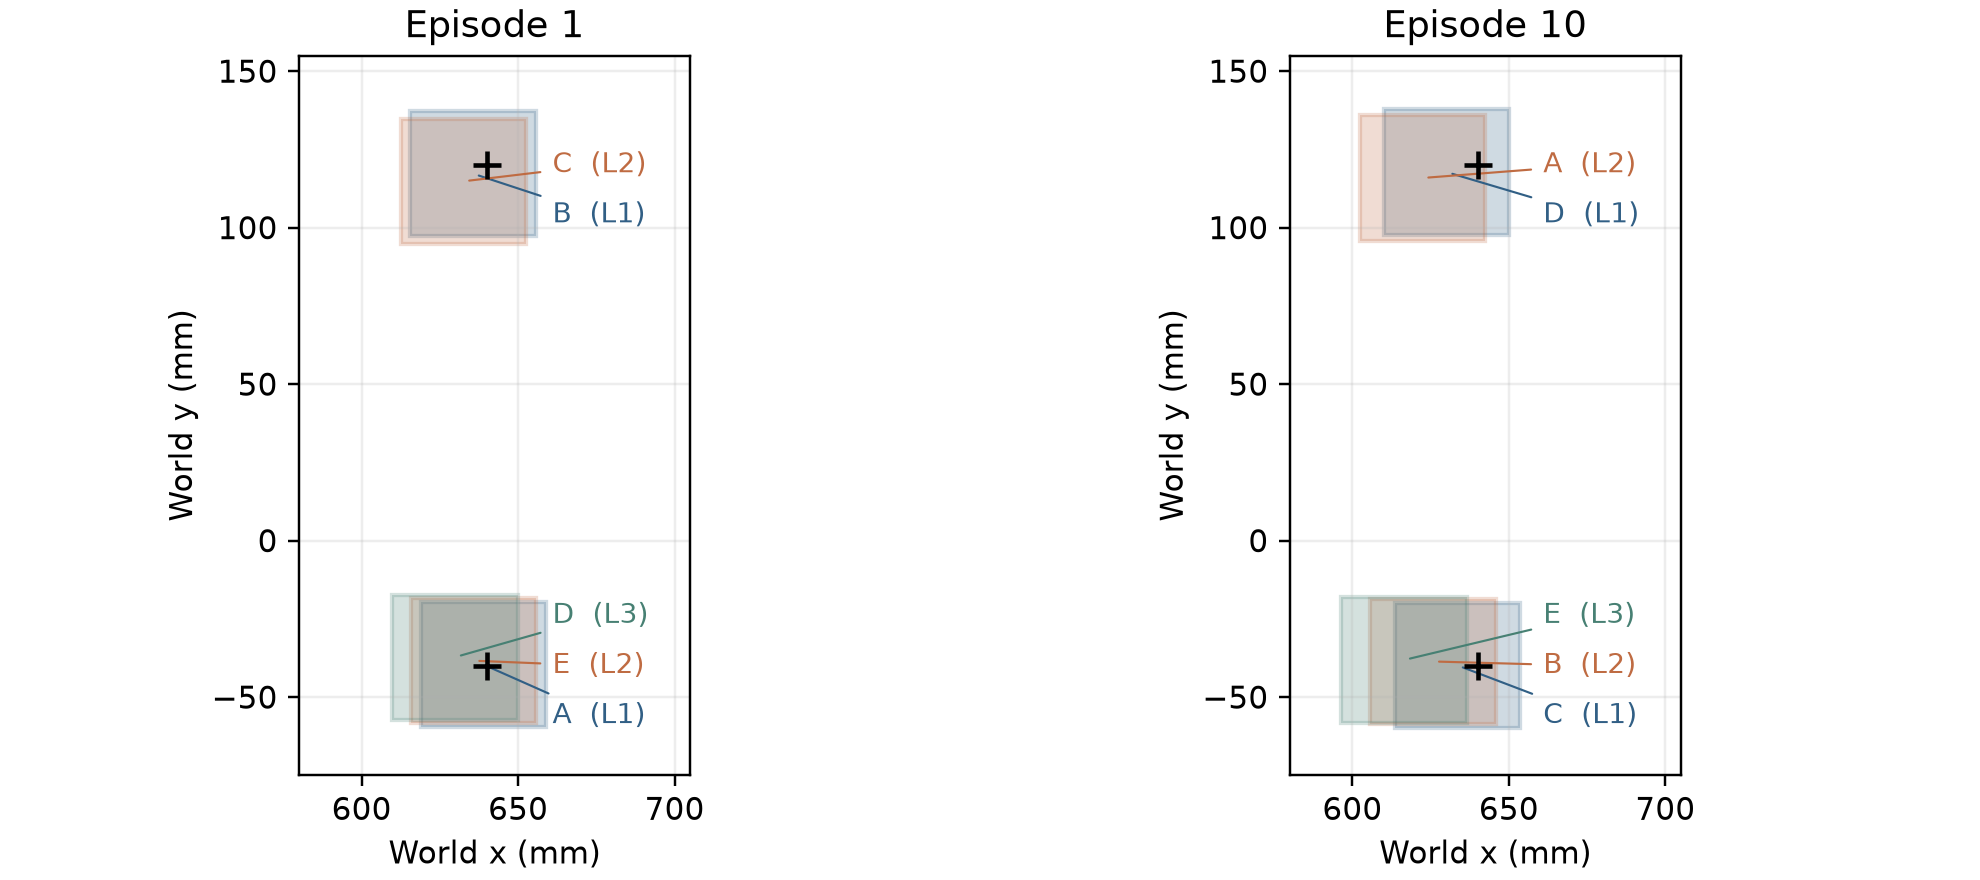
\includegraphics[width=.78\linewidth]{stacking_episodes.png}
\caption{Final layouts of two representative episodes from the archived evaluation logs. Letters identify blocks. Outlines are drawn to scale from logged block centres and show nominal cube width.}
\end{figure}

Placement error grew with tower height, driven primarily by horizontal offsets. Mean absolute vertical error stayed below 0.42 mm at each level. The raw correlation between pick sequence and placement error was 0.43 and fell to $-0.09$ after removing the mean effect of tower level. The level-adjusted correlations with initial $x$, absolute initial $y$, and pickup distance were $-0.23$, $0.15$ and $0.05$. With all ten runs successful, the data provide no comparison between successful and failed starts. At levels 1 and 2 the two-block tower had higher mean error, but tower size and target location were varied together.

Hand-tracking errors and block-placement errors measure different outcomes. In the ten randomized step logs, the episode-average peak hand position error was $58.16\pm3.76$ mm, the episode-average RMS hand position error was $26.32\pm0.85$ mm and the mean peak orientation error was $2.53\pm0.13^\circ$. No logged sample clipped the torque. These hand metrics include all motion and hold phases. The final placement metrics use the object centres after the episode.

\subsection{Phase timing and placement analysis}
For a stacking move of duration $T$, quintic timing uses $s=10u^3-15u^4+6u^5$ with $u=t/T$ clipped to $[0,1]$. Position is interpolated along a straight Cartesian segment. Both velocity and acceleration vanish at the endpoints, allowing a move to join a stationary gripper hold. The transit phases raise the carried block before traversing laterally, reducing interference with completed levels. After grasp closure and lift, the phase logic checks that the block rose at least 80 mm and that its offset relative to the hand is plausible before committing to transfer.

At level 1, the two- and three-block towers had mean errors of $10.11\pm0.09$ mm and $6.46\pm0.36$ mm, respectively. At level 2 their means were $17.83\pm0.24$ mm and $15.10\pm1.45$ mm. Because the towers have different fixed targets, the data cannot isolate a tower-size effect. The increase within both towers is consistent with residual placement bias and contact effects, but the final centre measurements do not identify the contribution of each phase. The per-level standard deviations pool repeated placements and therefore describe observed spread rather than independent uncertainty on a fitted height effect.

\begin{figure}[!htbp]
\centering
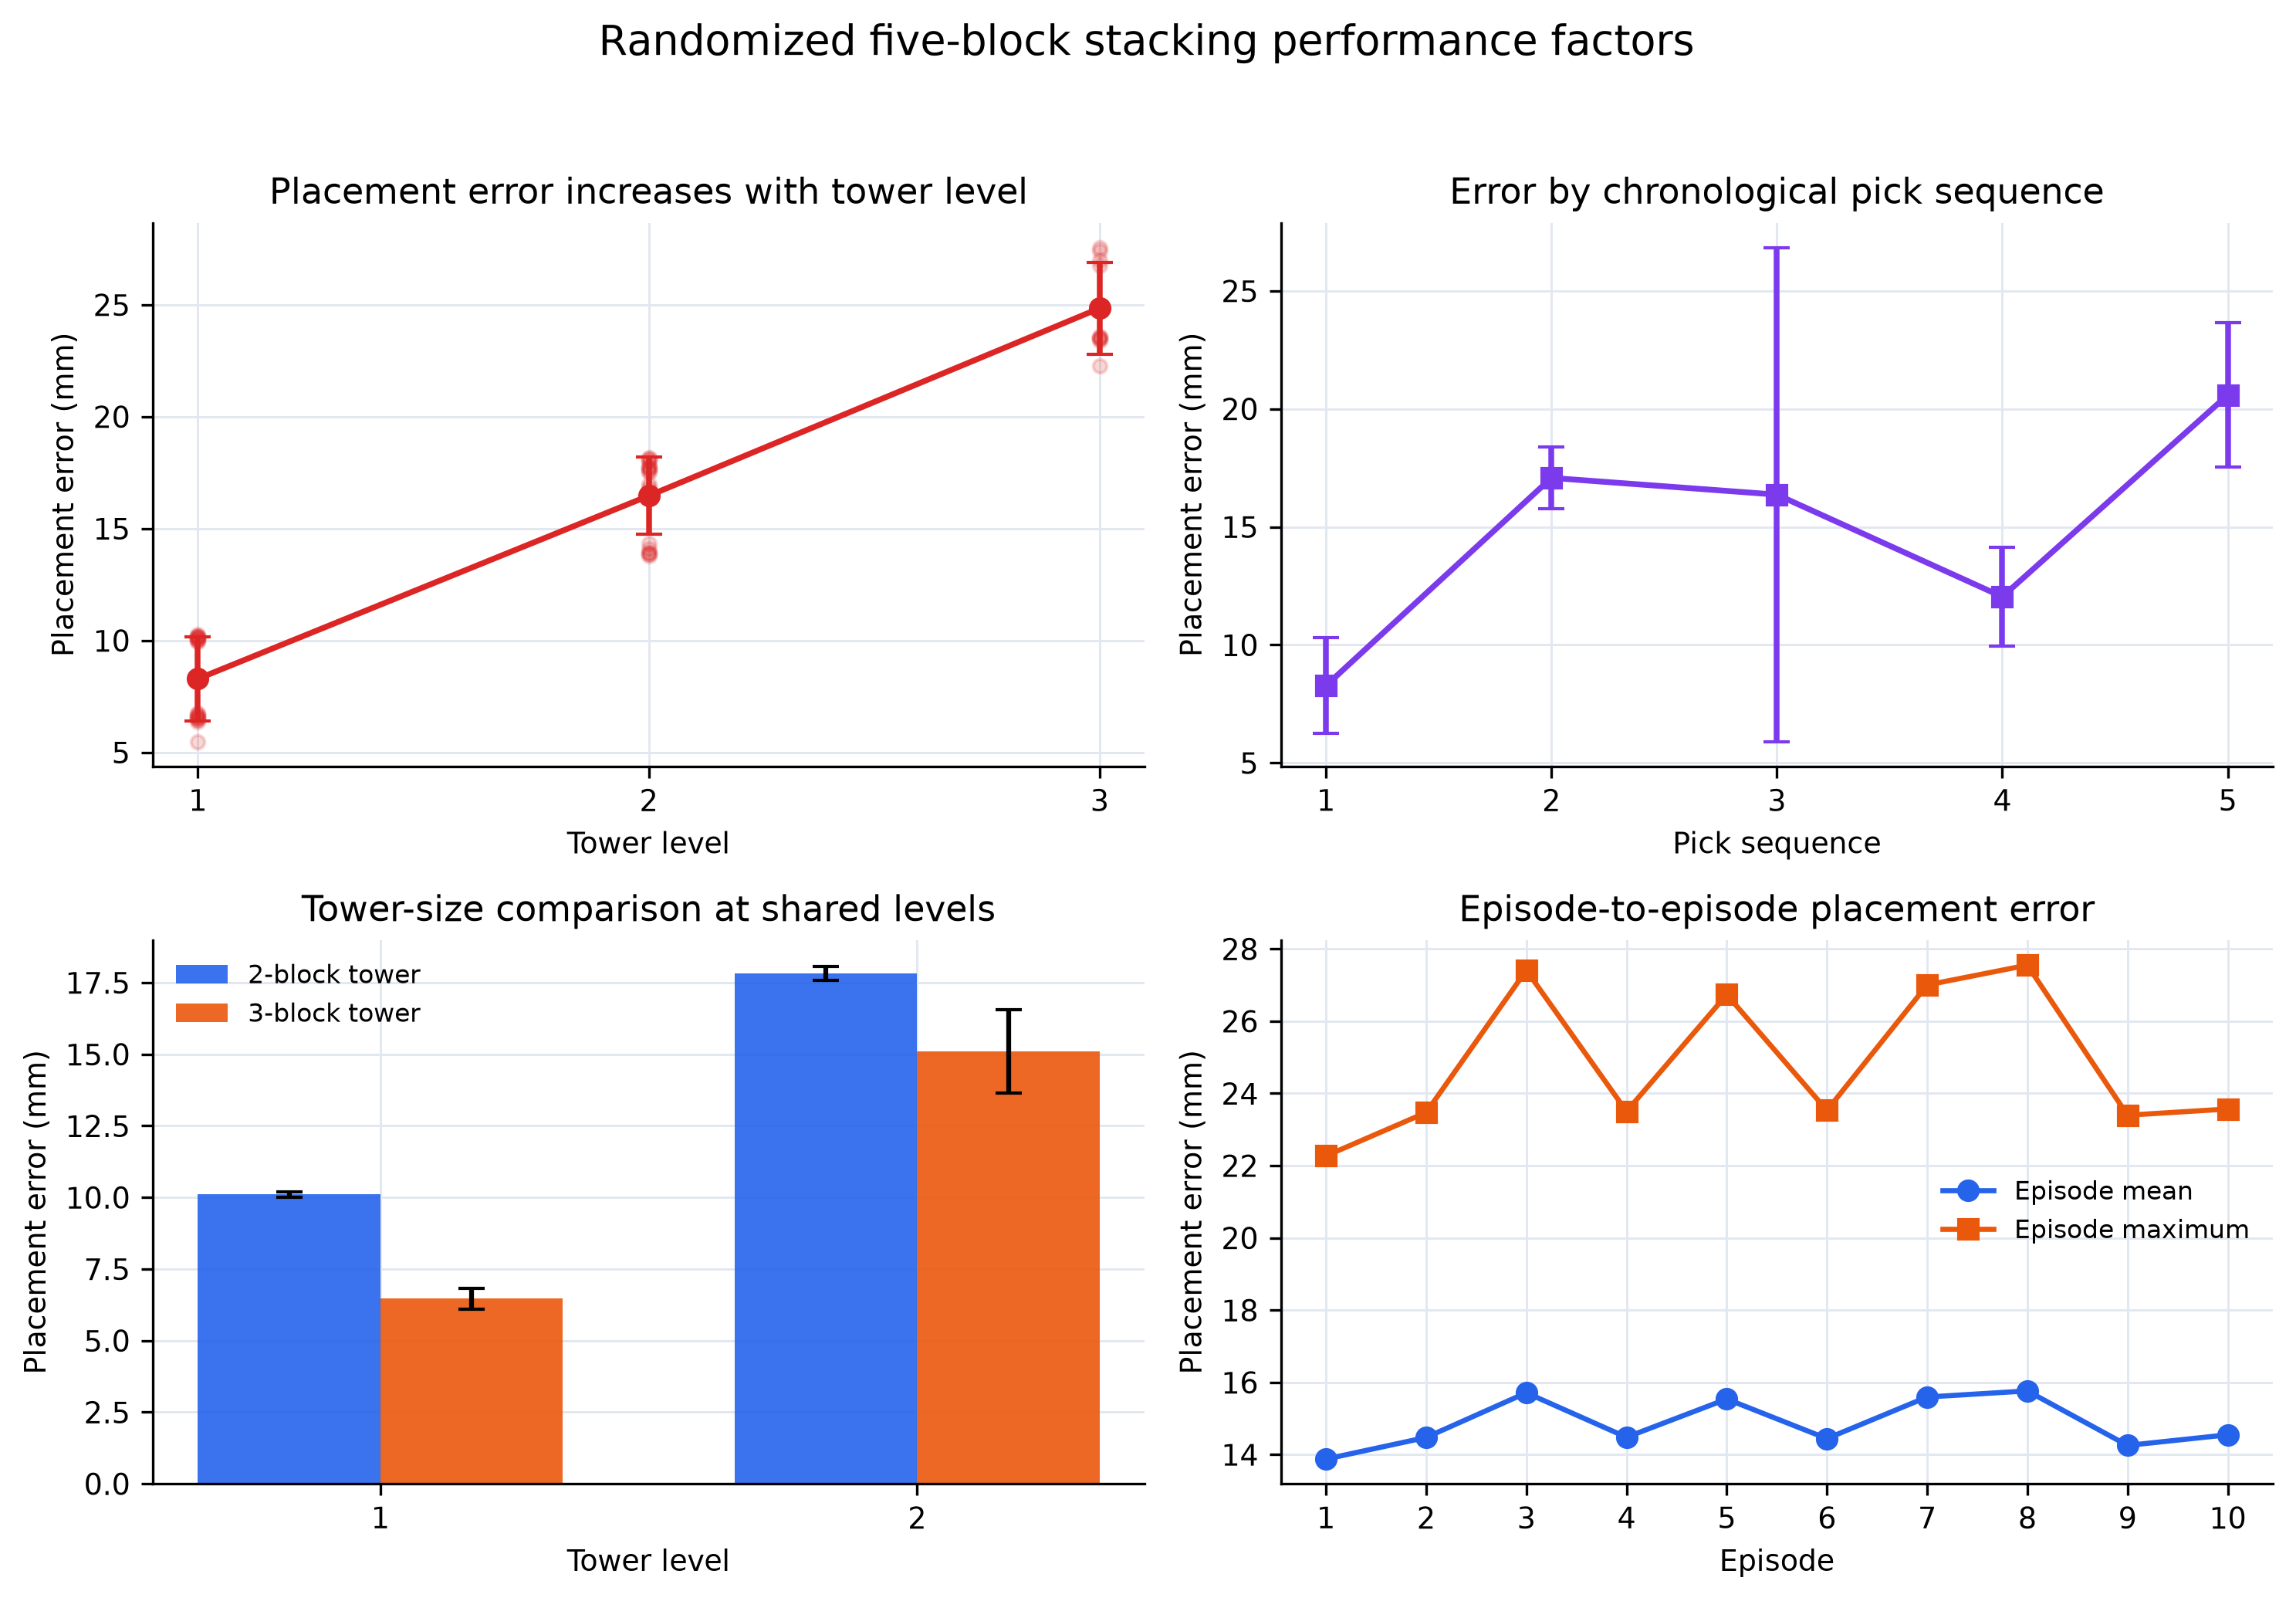
\includegraphics[width=.94\linewidth]{block_stacking_factor_analysis.png}
\caption{Placement errors grouped by tower level and tower configuration, with episode and pick-order comparisons.}
\label{fig:stack-factors}
\end{figure}

\subsection{Historical three-block baseline}
The earlier fixed-layout demonstration used these pickup centres (m).
\[
(0.55,0.00,0.42),\qquad (0.50,-0.14,0.42),\qquad (0.50,0.14,0.42).
\] All three blocks went to one tower at $(0.65,0.00)$ m with centre heights 0.42, 0.46 and 0.50 m. Its nine phases were approach, descend, grasp, lift, transfer, place, release, retreat and settle. The archive contains one run of 26,277 samples through 52.552 s. Each block passed the 35 mm horizontal and 25 mm vertical thresholds.

\begin{table}[!htbp]
\centering\small
\caption{Final placements in the archived fixed-layout run. The common target was $(0.65,0.00)$ m in the horizontal plane.}
\begin{tabular}{clrrr}
\toprule
Block & Final centre (m) & Target $z$ (m) & XY error (mm) & $|z|$ error (mm)\\
\midrule
1 & $(0.644816,0.000042,0.419814)$ & 0.42 & 5.18 & 0.19\\
2 & $(0.637755,0.001715,0.459706)$ & 0.46 & 12.36 & 0.29\\
3 & $(0.628142,-0.001871,0.499608)$ & 0.50 & 21.94 & 0.39\\
\bottomrule
\end{tabular}
\end{table}

Peak and RMS hand position errors in that run were 59.93 and 24.30 mm, peak orientation error was $2.65^\circ$, and no logged sample clipped torque. The historical baseline establishes the fixed-layout starting point for the project. The randomized experiment adds more blocks, different tower locations, different pickup orders and additional transit phases. The change in completion time therefore reflects a different task and phase schedule.

\FloatBarrier
\section{Discussion and Conclusion}
The Panda tracked all three tested path families at their nominal timing and completed the requested contact task across ten randomized layouts. The speed sweep and static load tests show two distinct limitations. Time compression increased trajectory error in the absence of clipping, and sustained load led to a static tracking offset. The first speed failures occurred below the monitored joint-speed and torque limits, which is consistent with finite tracking authority at the chosen gains as reference acceleration rises. A sustained unmodeled force creates equilibrium error under the PD law even with nominal bias compensation. Near a singularity, weaker Cartesian directions and the damped posture projection can change the response. The tests did not log singular values, so the observed errors cannot be attributed to singularities. The observed placement errors also increased with tower level despite level-specific calibration. The 35 mm horizontal criterion is generous relative to a 40 mm cube and should be considered when interpreting the success rate.

The results apply to the tested workspace and simulator model. The controller assumes exact object positions, uses a scripted phase sequence with grasp checks, and holds orientation fixed along the continuous paths. The orientation-step experiment evaluates rotational transients separately. Workspace boundaries, near-singular configurations, simultaneous position and orientation tracking, and real hardware remain outside the evaluated scope. Placement feedback and load compensation are direct extensions. PPO and SAC remain future work.

\section*{Reproducibility}
\addcontentsline{toc}{section}{Reproducibility}
\subsection*{Environment setup}
The experiments use Python 3.11 and were evaluated with MuJoCo 3.9.0. Use the full project repository, including the root \path{scene.xml} and the Panda XML and meshes under \path{assets/}. Keep this directory structure so the scene can resolve its model and mesh references.

From the repository root on macOS or Linux, create and activate a virtual environment and install the project dependencies.
\begin{samepage}
\begin{verbatim}
python3.11 -m venv venv
source venv/bin/activate
python -m pip install -r requirements.txt
python -c "import mujoco; print(mujoco.__version__)"
\end{verbatim}
\end{samepage}
The requirements file lists MuJoCo, NumPy, Gymnasium and Matplotlib. The version check records the installed simulator version because the requirements file specifies minimum versions. The first command in the next section validates the loaded model and kinematics without opening a viewer.

\subsection*{Running the experiments}
Run the following from the repository root with the project environment active. The experiment scripts save per-run data and summaries under \texttt{results/}.
\begin{verbatim}
python validate_kinematics.py
python simulation_task_space_pd.py --headless --no-realtime
python trajectory_following.py --headless --seed 19
python trajectory_experiments.py --headless
python plot_trajectory_study_results.py
python step_response_experiments.py
python speed_limit_experiments.py
python robustness_experiments.py
python plot_controller_limit_results.py
python simulation_grasp_lift.py --headless --no-realtime
python simulation_block_stacking.py --headless --save-step-logs
python analyze_block_stacking_results.py
\end{verbatim}
The IK table is saved at \path{results/logs/ik_validation_results.csv}. The trajectory study writes per-run CSV metrics and NPZ time series. Stacking writes \path{episodes.csv} and the optional step logs under \path{results/block_stacking/}. That directory also holds the historical \path{block_stacking_log.csv}. Single-episode replays save their output under \path{results/block_stacking/replays/}. On macOS, run the passive viewer with \texttt{mjpython}.
\begin{verbatim}
mjpython simulation_block_stacking.py --episode 2 --seed 42
\end{verbatim}

\appendix
\section{Implementation Excerpts}
The excerpts below document the numerical interfaces used by the experiments. The environment returns a pose object with position and rotation. Forward kinematics evaluates a candidate configuration by restoring the live generalized position and velocity in a \texttt{finally} block. The Jacobian keeps the seven arm velocity columns, excluding the gripper and free-body joints.

\begin{lstlisting}[caption={State-preserving forward kinematics and arm Jacobian from the environment.}]
def forward_kinematics(self, q: Optional[np.ndarray] = None) -> Pose:
    """Return MuJoCo's end-effector pose for q without permanently changing state."""
    if q is None:
        mujoco.mj_forward(self.model, self.data)
        return self.get_end_effector_pose()
    q = np.asarray(q, dtype=float)
    if q.shape != (7,):
        raise ValueError("q must have shape (7,).")
    saved_qpos = self.data.qpos.copy()
    saved_qvel = self.data.qvel.copy()
    try:
        self.data.qpos[self.arm_qpos_indices] = q
        self.data.qvel[:] = 0.0
        mujoco.mj_forward(self.model, self.data)
        return self.get_end_effector_pose()
    finally:
        self.data.qpos[:] = saved_qpos
        self.data.qvel[:] = saved_qvel
        mujoco.mj_forward(self.model, self.data)

def geometric_jacobian(self) -> np.ndarray:
    jac_pos = np.zeros((3, self.model.nv))
    jac_rot = np.zeros((3, self.model.nv))
    mujoco.mj_jacBody(
        self.model, self.data, jac_pos, jac_rot, self.end_effector_body_id
    )
    return np.vstack(
        [jac_pos[:, self.arm_dof_indices], jac_rot[:, self.arm_dof_indices]]
    )

\end{lstlisting}

The IK iteration checks both pose tolerances before computing a damped correction. The preferred-posture bias is projected before the total update is norm-limited and clipped to the joint bounds.

\begin{lstlisting}[caption={Convergence test and damped least-squares update inside the IK loop.}]
if pos_norm <= position_tol and rot_norm <= orientation_tol:
    converged = True
    break

error = np.concatenate([pos_error, rot_error])
jacobian = self.geometric_jacobian()
regularized = jacobian @ jacobian.T + damping**2 * np.eye(6)
jacobian_pinv = jacobian.T @ np.linalg.solve(regularized, np.eye(6))
null_projector = np.eye(7) - jacobian_pinv @ jacobian
delta_q = jacobian_pinv @ error + nullspace_gain * null_projector @ (preferred_q - q)

norm = np.linalg.norm(delta_q)
if norm > max_update_norm:
    delta_q *= max_update_norm / norm
q = np.clip(q + step_size * delta_q, lower, upper)
\end{lstlisting}

The final torque calculation shows how the Cartesian wrench, posture correction and bias compensation are combined before clipping. The inverse is formed through a linear solve in task-space dimensions.

\begin{lstlisting}[caption={Torque mapping, damped posture projection and actuator clipping.}]
task_torque = jacobian.T @ task_wrench

# Damped projector keeps the secondary posture command from strongly
# disturbing the primary six-dimensional end-effector task.
regularized = jacobian @ jacobian.T + config.damping**2 * np.eye(6)
jacobian_pinv = jacobian.T @ np.linalg.solve(regularized, np.eye(6))
null_projector = np.eye(7) - jacobian_pinv @ jacobian
if preferred_q is None:
    preferred_q = q.copy()
else:
    preferred_q = np.asarray(preferred_q, dtype=float).reshape(7)
posture_torque = null_projector.T @ (
    config.nullspace_kp * (preferred_q - q)
    - config.nullspace_kd * qd
)

# qfrc_bias contains gravity, Coriolis, and centrifugal bias forces.
bias_torque = self.data.qfrc_bias[self.arm_dof_indices].copy()
raw_torque = task_torque + posture_torque + bias_torque
torque = np.clip(raw_torque, -config.torque_limits, config.torque_limits)
\end{lstlisting}

The quintic reference supplies position, velocity and acceleration to downstream phase logic. Keeping the timing function separate from the move endpoints lets each phase share the same endpoint conditions.

\begin{lstlisting}[caption={Quintic time scaling used by the stacking phase generator.}]


def quintic_scaling(t: float, duration: float) -> tuple[float, float, float]:
    """Return s, s_dot and s_ddot with zero endpoint velocity/acceleration."""
    tau = np.clip(t / duration, 0.0, 1.0)
    s = 10 * tau**3 - 15 * tau**4 + 6 * tau**5
    sd = (30 * tau**2 - 60 * tau**3 + 30 * tau**4) / duration
    sdd = (60 * tau - 180 * tau**2 + 120 * tau**3) / duration**2
    return float(s), float(sd), float(sdd)
\end{lstlisting}

\begin{thebibliography}{9}

\bibitem{khatib1987}
O.~Khatib,
``A unified approach for motion and force control of robot manipulators: The operational space formulation,''
\emph{IEEE Journal on Robotics and Automation}, vol.~3, no.~1, pp.~43--53, 1987.
doi: \href{https://doi.org/10.1109/JRA.1987.1087068}{10.1109/JRA.1987.1087068}.

\bibitem{todorov2012}
E.~Todorov, T.~Erez, and Y.~Tassa,
``MuJoCo: A physics engine for model-based control,''
in \emph{2012 IEEE/RSJ International Conference on Intelligent Robots and Systems},
pp.~5026--5033, 2012.
doi: \href{https://doi.org/10.1109/IROS.2012.6386109}{10.1109/IROS.2012.6386109}.


\bibitem{menageriePanda}
Google DeepMind, ``Franka Emika Panda description (MJCF),''
\emph{MuJoCo Menagerie}, model documentation.
\href{https://github.com/google-deepmind/mujoco_menagerie/blob/main/franka_emika_panda/README.md}{Model source and documentation}.
Accessed 19 November 2026.

\bibitem{wampler1986}
C.~W. Wampler,
``Manipulator inverse kinematic solutions based on vector formulations and damped least-squares methods,''
\emph{IEEE Transactions on Systems, Man, and Cybernetics}, vol.~SMC-16, no.~1, pp.~93--101, 1986.
doi: \href{https://doi.org/10.1109/TSMC.1986.289285}{10.1109/TSMC.1986.289285}.

\bibitem{siciliano2009}
B.~Siciliano, L.~Sciavicco, L.~Villani, and G.~Oriolo,
\emph{Robotics: Modelling, Planning and Control}.
Springer, 2009. doi: \href{https://doi.org/10.1007/978-1-84628-642-1}{10.1007/978-1-84628-642-1}.
\end{thebibliography}
\end{document}
